\section{Overview}

We are presenting here the results from our experiments over a period of 100 days, from the August 1st 2013 to November 9th, 2013. During this period, we collected 9.5 GB of raw HTTP requests, consisting in approximately 11.0M GET and 1.9M POST. Our honeypots were visited by more than 73,000 different IP addresses, spanning 178 countries and presenting themselves with more than 11,000 distinct User-Agents. This is over one order of magnitude larger than what has been observed in the previous study by John et al. on low interaction web-application honeypots \cite{johnhsh}. Moreover, we also extracted over 110,000 files that were uploaded or modified during attacks against our websites, 85,000 of them are unique.

There are two different ways to look at the data we collected: one is to identify and study attacks looking at the web server logs, and the other one is to try to associate a goal to each of them by analyzing the uploaded and modified files. In the first part of this chapter we will look at the first part, while in the second we will give some examples of uploaded files, in order to understand attacker's goals.

\section{Attack Session: the 4 phases}

While analyzing the behaviour of attackers lured by our honeypots, we identified four different phases commonly present in an attack session: discovery, reconnaissance, exploitation, and post-exploitation. The \emph{Discovery} phase describes how attackers find their targets, e.g. by querying a search engine (using a dork) or by simply scanning IP addresses. The \emph{Reconnaissance} phase contains information related to the way in which the pages were visited, for instance by using automated crawlers or by manual access, and if this manual access is performed via visual browser or command line tool, and if the attacker is using an anonymization proxy. In the \emph{Exploitation} phase we describe the number and types of actual attacks performed against our web applications. Some of the attacks reach their final goal themselves (for instance by changing a page to redirect to a malicious website), while others are only uploading a second stage. In this case, the uploaded file is often a web shell that is later used by the attacker to manually log in to the compromised system and continue the attack. We refer to this later stage as the \emph{Post-Exploitation} phase.

It must be noticed, however, that not all phases are present in every attack: some of them can be joined in one step (e.g., reconnaissance and exploitation are often performed in one single action), some of them are simply not present (e.g, post-exploitation), some visits do not lead to an actual attack (errors in attackers requests, or incomplete file uploads), and sometimes it is just impossible to link together different actions performed by the same attacker with different IP addresses.

Nevertheless, by extracting the most common patterns from the data collected at each stage, we can identify the ``typical attack profile'' observed during our experiments with the following sequence:

\begin{enumerate}
\item
69.8\% of the attacks start with a scout bot visiting the page. The scout often tries to hide its User Agent (removing directly the header) or disguise themselves as a crawler search (the most used being \emph{GoogleBot});
\item
Few seconds after the scout has identified the page as an interesting target, a second automated system (hereinafter exploitation bot) visits the page and executes the real exploit. This is often a separate script that does not fake the user agent, therefore often appearing with strings such as \emph{libwww/perl}.
\item
If the vulnerability allows the attacker to upload a file, in 46\% of the cases the exploitation bot uploads a web shell. Moreover, the majority of the attacks uploads the same file multiple times (in average 9, and sometimes up to 40), probably to be sure that the attack was successful.
\item
After an average of 3 hours and 26 minutes, the attacker logs into the machine using the previously uploaded shell. The average login time for an attacker interactive session is 5 minutes and 37 seconds.
\end{enumerate}

While this represents the most common behaviour extracted from our dataset, many other combinations were observed as well - some of which are described in the rest of the section. Finally, it is important to mention that the attack behaviour may change depending on the application and on the vulnerability that is exploited. Therefore, we should say that the previous description summarizes the most common behaviour of attacks against osCommerce 2.2 (the web application that received by far the largest number of attacks among our honeypots). A particular notice must be performed regarding the SMF application: this application suffered from heavy traffic, provoked by automated bots, and we preferred to exclude this application from our statistics in order to produce more reliable results. A specific discussion over the content of messages posted on the forum will be performed later. In Figure ~\ref{fig:overview_phases} we show an overview of the four phases and its characteristics.

\begin{figure}[tbh]
\centerline{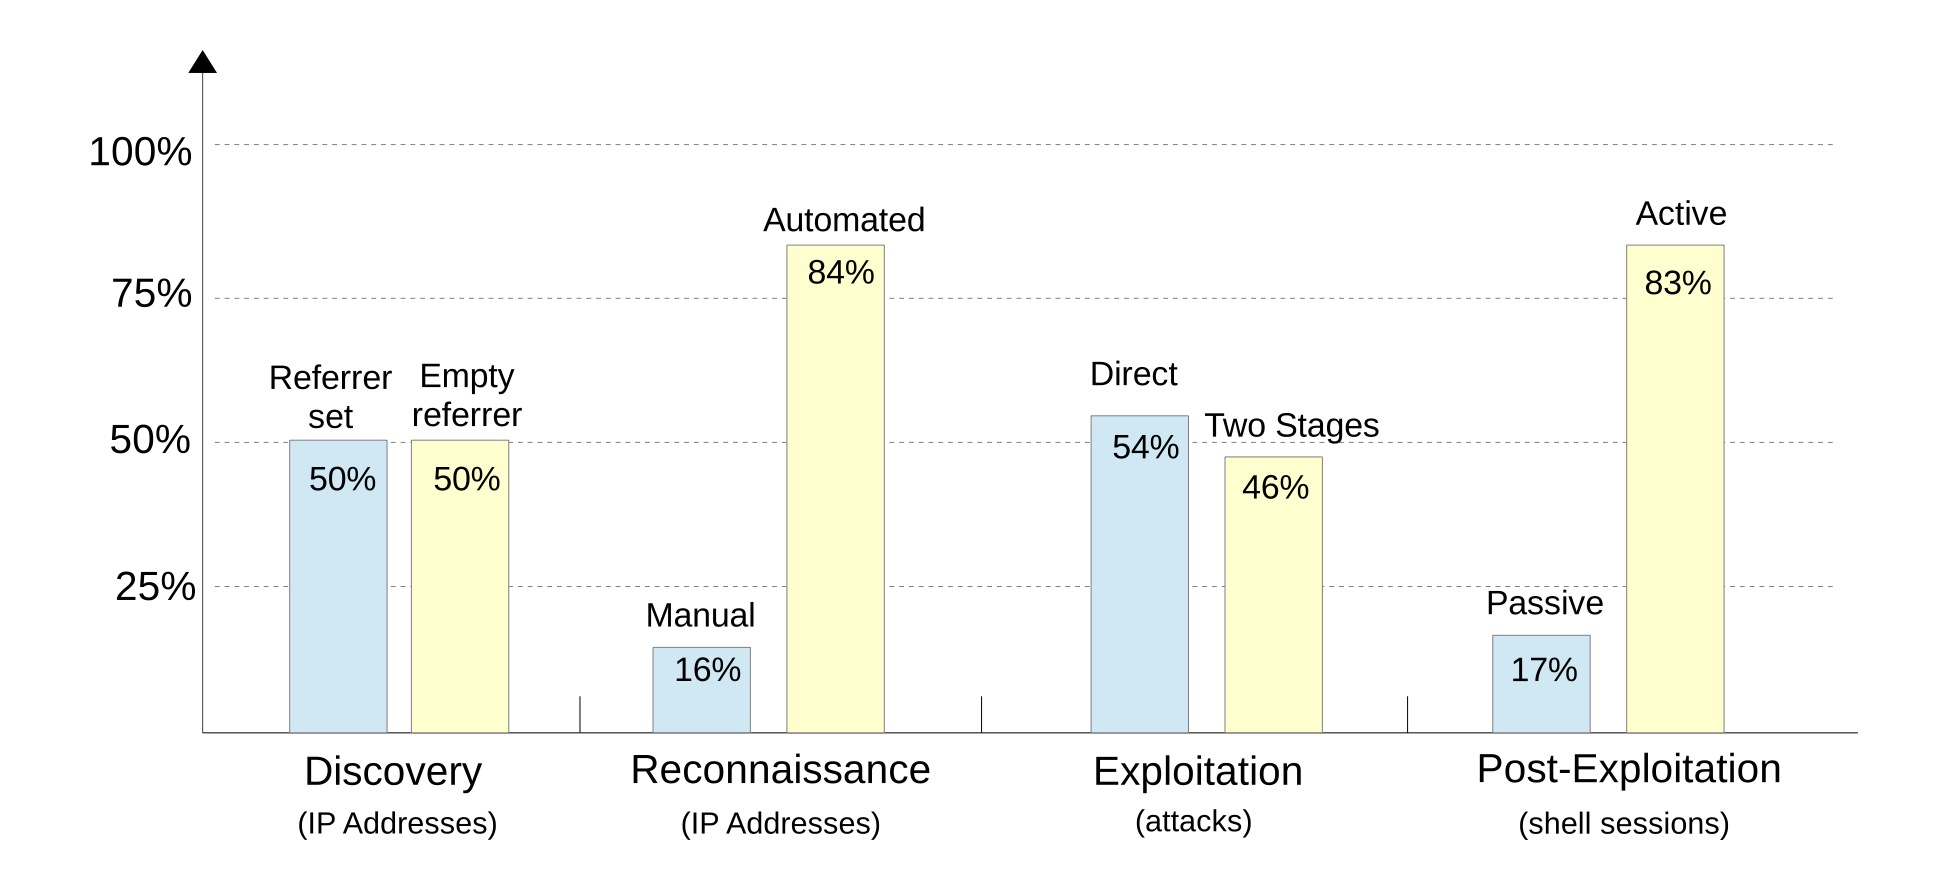
\includegraphics[scale=0.4]{Images/overview_phases.jpg}}
\caption{Overview of the four phases of an attack\label{fig:overview_phases}}
\end{figure}

\subsection{Discovery}
The very first HTTP request hit our HoneyProxy only 10 minutes after the deployment, from ``Googlebot''. The first request not related to a benign crawler came after 1 hour and 50 minutes.
During the first few days, most of the traffic was caused by benign web crawlers. Therefore, we designed a simple solution to filter out benign crawler-generated traffic from the remaining traffic. Since HTTP headers alone are not trustable (e.g., attackers often use User Agents such as ``Googlebot'' in their scripts) we collected public information available on bots and we combined them with information extracted from our logs and validated with WHOIS results in order to identify crawlers from known companies. By combining User Agent strings and the IP address ranges associated to known companies, we were able to identify with certainty 14 different crawlers, originating from 1965 different IPs. Even though this is not a complete list, it was able to successfully filter out most of the traffic generated by benign crawlers.

\begin{figure}[tbh]
\centerline{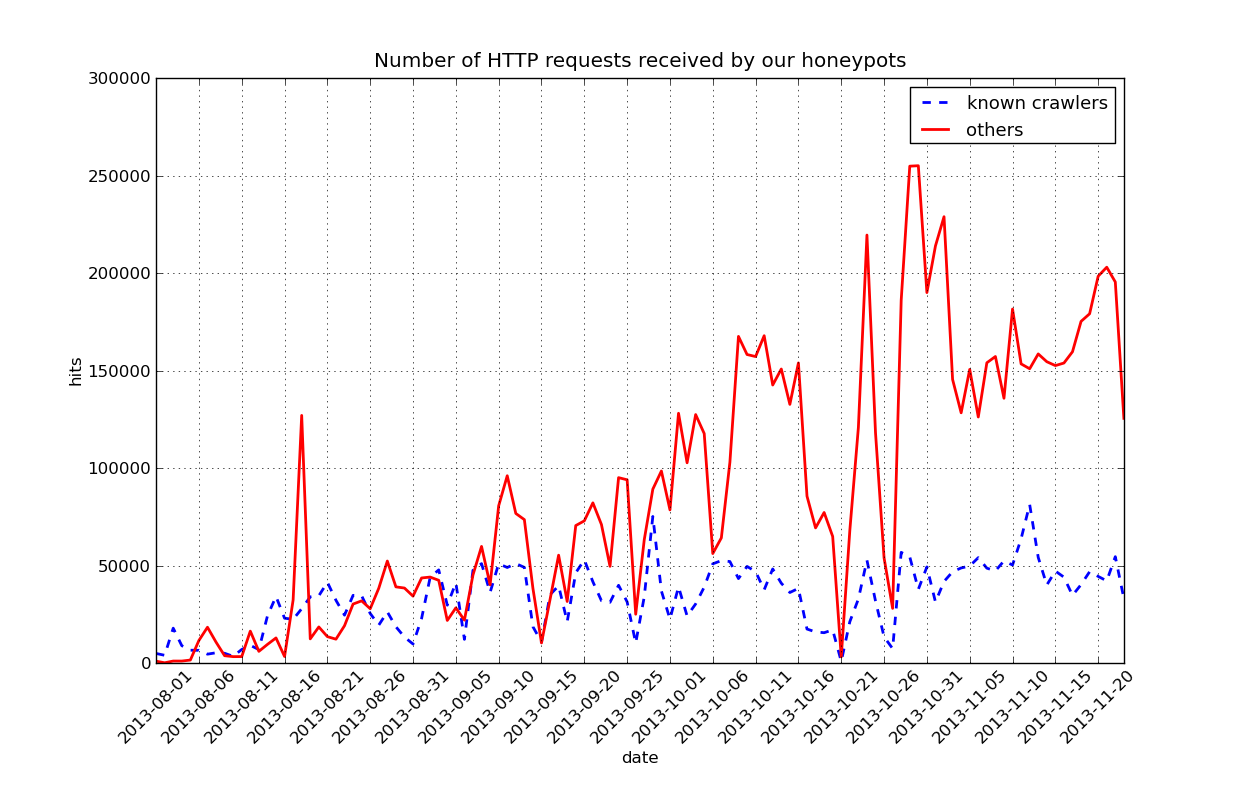
\includegraphics[scale=0.4]{Images/requestsCrawlers.png}}
\caption{Overview of HTTP requests received by our honeypots\label{fig:requestsCrawlers}}
\end{figure}

Some statistics about the origin of the requests is shown in Figure ~\ref{fig:requestsCrawlers}. The amount of legitimate crawler requests is more or less stable in time, while, as time goes by and the honeypot websites get indexed by search engines and linked on hacking forums or on link farming networks, the number of requests by malicious bots or non-crawlers has an almost linear increase.
While looking at these statistics we also noticed a number of suspicious spikes in the number of accesses. In several cases, one of our web applications was visited, in few hours, by several thousands of unique IP addresses (compared with an average of 192 per day), a clear indication that a botnet was used to scan our sites.

Interestingly, we observed the first suspicious activity only 2 hours and 10 minutes after the deployment of our system, when our forum web application started receiving few automated registrations. However, the first posts on the forum appeared only four days later, on December 27th. Even more surprising was the fact that the first visit from a non-crawler coincided with the first attack: 4 hours 30 minutes after the deployment of the honeypots, a browser with Polish locale visited our osCommerce web application and exploited a file upload vulnerability to upload a malicious PHP script to the honeypot. We also examined the IP source address in order to understand the more active countries, as we can see from ~\ref{fig:requests_countries} China, Russia, and USA are in order the top three countries for number of requests.

\begin{figure}[tbh]
\centerline{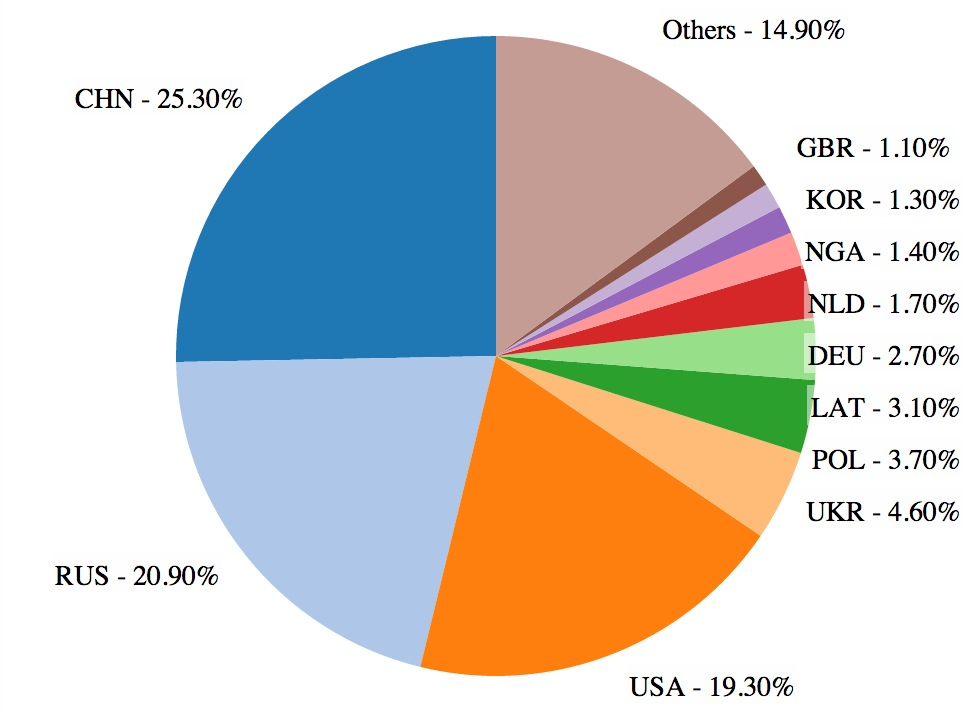
\includegraphics[scale=0.7]{Images/requests_countries.jpg}}
\caption{Number of requests divided by country\label{fig:requests_countries}}
\end{figure}

\subsubsection{Referrer Analysis}

The analysis of the Referrer HTTP header (whenever available) helped us identify how visitors were able to find our honeypots on the web. Based on the results, we can distinguish two main categories of users: attackers using search engines to find vulnerable applications, and victims of phishing attacks following links posted in emails and public forums.
A total of 66,449 visitors reached our honeypot pages with the Referrer header set. The domains appearing most frequently as referrers are search engines, followed by web mails and public forums. Google is leading with 17,156 entries. Other important search engines used by the attackers to locate our websites, were Yandex (1,016), a Russian search engine, Bing (263), Microsoft search engine, and Yahoo (98). A total of 7,325 visitors arrived from web mail services (4,776 from SFR, 972 from Facebook, 944 from Yahoo! Mail, 493 from Live.com, 407 from AOL Mail, and 108 from comcast.net). Finally, 15,746 requests originated from public web forums, partially belonging to hacking communities, and partially just targeted by spam bots.

Finally, we extracted search queries (also known as ``dorks'', when used for malicious purposes) from Referrer headers set by the most common web search engines. Our analysis shows that the search terms used by attackers highly depend on the application deployed on the honeypot. For example, the most common dork that was used to reach our Joomla web application contained the words \emph{``joomla allows you''}, while the Simple Machines Forum was often reached by searching \emph{``powered by smf''}. Our machine containing public web shells was often reached via dorks like \emph{``inurl:c99.php''}, \emph{``cyber anarchy shell''} or even \emph{``ftp AND brute-forcer AND security AND info AND processes AND mysql AND php-code AND en-coder AND backdoor AND back-connection AND home AND enumerate AND md5-lookup AND word-lists AND milw0rm AND itsearch AND self-kill AND about''}. The latter query, even though very long, was used more than 150 times to reach our machine with web shells. It was probably preferred to searching via \emph{``intitle:''} or \emph{``inurl:''} because attackers tend to customize names and titles of the scripts, therefore a search for direct text content may return more results. Some specialized search engines appear to be used as well, such as devilfinder.com \cite{devilfinder}, which was adopted in 141 cases to reach some of the shells on our machines. This search engine claims to show more low-ranking results than common search engines, not to store any search data, and to return up to 300 results on the same web page, making it very suitable for attackers willing to search for dorks and collect long lists of vulnerable websites.

\subsection{Reconnaissance}

After removing the legitimate crawlers, the largest part of the traffic received by our honeypots came from unidentified sources, many of which were responsible of sending automated HTTP requests. We found these sources to be responsible for the majority of attacks and spam messages targeting our honeypots during our experiments.

However, distinguishing attackers that manually visited our applications from the ones that employed automated scout bots is not an easy task. We applied the following three rules to flag the automated requests:

\begin{description}
\item[Inter-arrival time.] If requests from the same IP address arrive at a frequency higher than a certain threshold, we consider the traffic as originated from a possible malicious bot.
\item[Request of images.] Automated systems, and especially those having to optimize their speed, almost never request images or other presentation-related content from websites. Scanning web logs for visitors that never request images or CSS content is thus an easy way of spotting possible automated scanners.
\item[Subdomain visit pattern.] As described in Chapter 1, each website we deployed consisted in a number of subdomains linked together according to a predetermined pattern. If the same IP accesses them in a short time frame, following our patterns, then it is likely to be an automated crawler.
\end{description}

For example, after removing the benign crawlers, a total of 9.5M hits were received by systems who did not request any image, against 1.8M from system that also requested images and presentation content. On the contrary, only 641 IP addresses (responsible for 13.4K hits) visited our websites by following our links in a precise access pattern. Among them, 60\% followed a breadth first approach.
85\% of the automated requests were directed to our forum web application, and were responsible for registering fake user profiles and posting spam messages. Of the remaining 1.4M requests directed to the seven remaining honeypot applications, 95K were mimicking the User-Agent of known search engines, and 264K switched between multiple User-Agents over time. The remaining requests did not contain any suspicious User-Agent string, did not follow paths between domains, neither requested images. As such, we classified them as unknown (possibly benign) bots.

\subsection{Exploitation}

The first important activity we performed in order to detect exploitation attempts was parsing the log files in search of attack traces. Luckily, knowing already the vulnerabilities affecting our web applications allowed us to quickly and reliably scan for attacks in our logs using a set of regular expressions.
Overall, we logged 444 distinct exploitation sessions. An interesting finding is that 310 of them adopted two or more different User-Agent strings, appearing in short sequence from the same IP address. As explained before, this often happens when attackers employ a combination of scout bots and automatic attack scripts in order to speed up attacks and quickly find new targets. In particular, in two thirds (294) of the total exploitation sessions we observed, the User-Agent used for the exploitation was the one associated to the LibWWW Perl library (libwww/perl).
In some of these exploitation sessions, the attacker tried to disguise her tools and browser as known benign bots. Some crawler User-Agent strings that were often used during exploitation sessions were: ``FreeWebMonitoring'', ``Gigabot/3.0'', ``gsa-crawler'', ``IlTrovatore-Setaccio/1.2'', ``bing- bot/2.0;'', and ``Googlebot/2.1''.

\begin{figure}[tbh]
\centerline{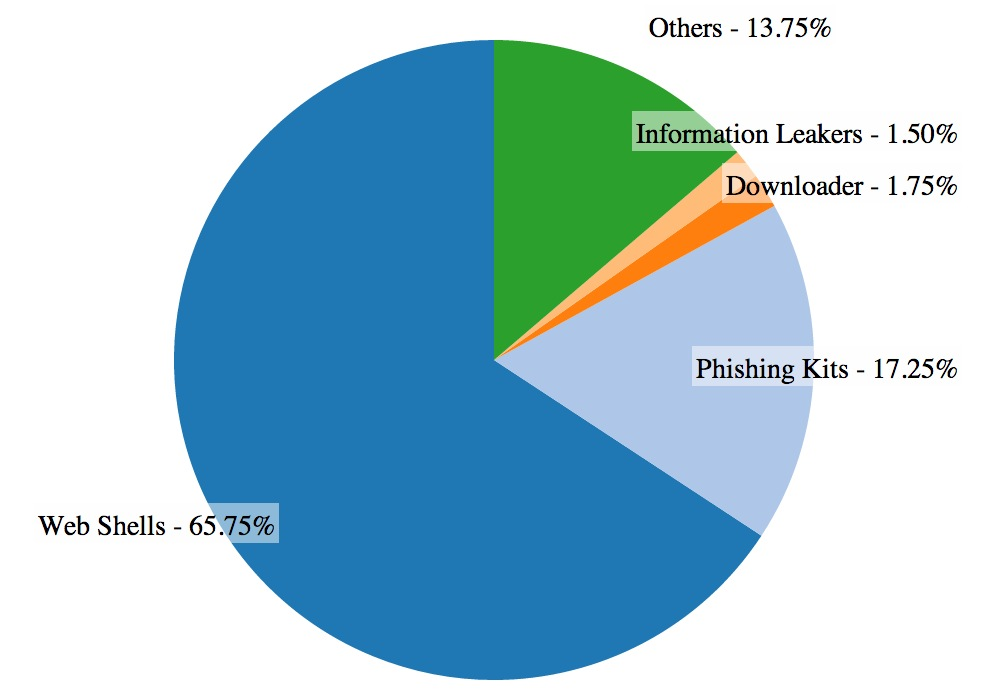
\includegraphics[width=0.8\textwidth]{Images/1stStageAttack.jpg}}
\caption{1st Stage attack file categorization.\label{fig:1stStageAttack}}
\end{figure}

The most remarkable side effect of every exploitation session is the upload or modification of files on the victim machine. Quite surprisingly, we noticed that when an exploitation session uploads a file, the file is uploaded in average 9.75 times. This strange behaviour can be explained by the fact that most of the exploitation tools are automated, and since the attacker does not check in real-time whether each exploit succeeded or not, uploading the same file multiple times can increase the chance for the file to be successfully uploaded at least once. Results of this phase, resumed in Figure~\ref{fig:1stStageAttack}, show that the files uploaded during attack sessions consist, in 65.75\% of the cases, in web shells, in 17.25\% of the cases in phishing packs (single HTML pages or complete phishing kits), in 1.75\% of the cases in scripts that automatically try to download and execute files from remote URLs, and in 1.5\% of the cases in scripts for local information gathering. The remaining 13.75\% of the files include malwares, defacement pages and several other categories.

\begin{figure}[tbh]
\centerline{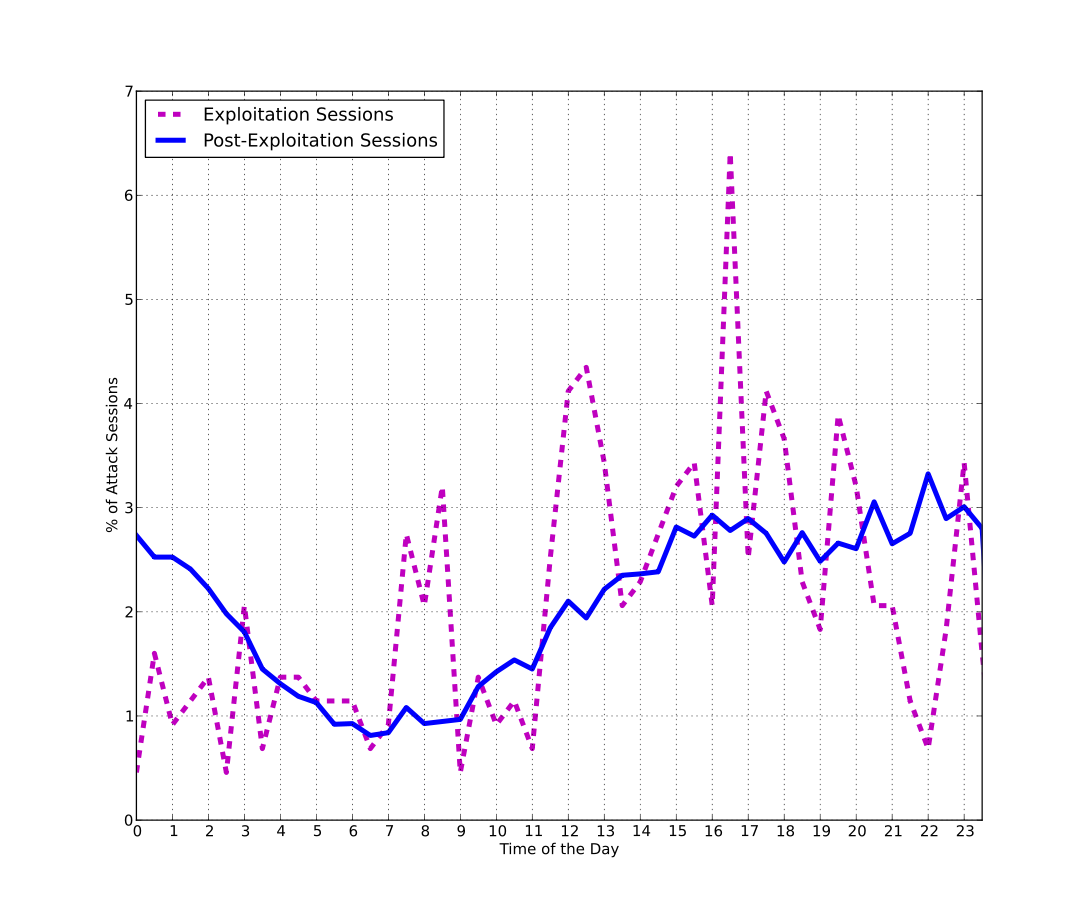
\includegraphics[width=0.8\textwidth]{Images/normalizedAttackTimes.png}}
\caption{Normalized time of attack sessions.\label{fig:normalizedAttackTimes}}
\end{figure}

Figure~\ref{fig:normalizedAttackTimes} shows the normalized times of the attacks received by our honeypots. The values were computed by adjusting the actual time of the attack with the time zone extracted from the IP geolocalization. It must be noticed that, using this method, we can have some false values in case the attacker is proxying its connection through an IP in a different part of the world. However, the graph shows a clear daylight trend for both the exploitation and post-exploitation phases. In particular, for the interactive sessions we observed fewer attacks performed between 4am and 10am, when probably also criminals need to get some sleep. Interestingly, also the exploitation phase, that is mostly automated, shows a similar trend (even though not as clear). This could be the consequence of scans performed by botnet infected machines, some of which are probably turned off by their users during the night.

\subsubsection{Forum Activity}

Since the 1st day of operation, our forum application received a very large amount of traffic. Most of it came from automated spamming bots that kept flooding the forum with fake registrations and spam messages. We analysed every snapshot of the machine's database in order to extract information about the forum's posts and the URLs that were embedded in each of them. This allowed us to identify and categorize several spam and link farming campaigns, as well as finding some rogue practices such as selling forum accounts.

A total of 68,201 unique messages were posted on the forum during our study, by 15,753 users using 3,144 unique IP addresses. Daily statistics on the forum show trends that are typical of medium to high traffic message boards: an average of 604 posts per day (with a max of 3085), with an average of 232 online users during peak hours (max 403).
Even more surprising than the number of posts is the number of new users registered to the forum: 1907 per day in average, and reaching a peak of 14,400 on October 23, 2013. We measured that 33.8\% of IP addresses that performed actions on our forum were responsible of creating at least one fake account, but never posted any message. This finding suggests there are some incentives for criminals to perform automatic user registrations, and perhaps selling user accounts is even more profitable than the spamming activity itself. Our hypothesis is that, in some cases, forum accounts can be sold in bulk to other actors in the black market. We indeed found 1,260 fake accounts that were created from an IP address and then used few days later by other, different IPs, to post messages. This does not necessarily validate our hypothesis, but shows at least that forum spamming has become a complex ecosystem and it is difficult, nowadays, to find only a single actor behind a spam or link farming campaign.

\begin{figure}[tbh]
\centerline{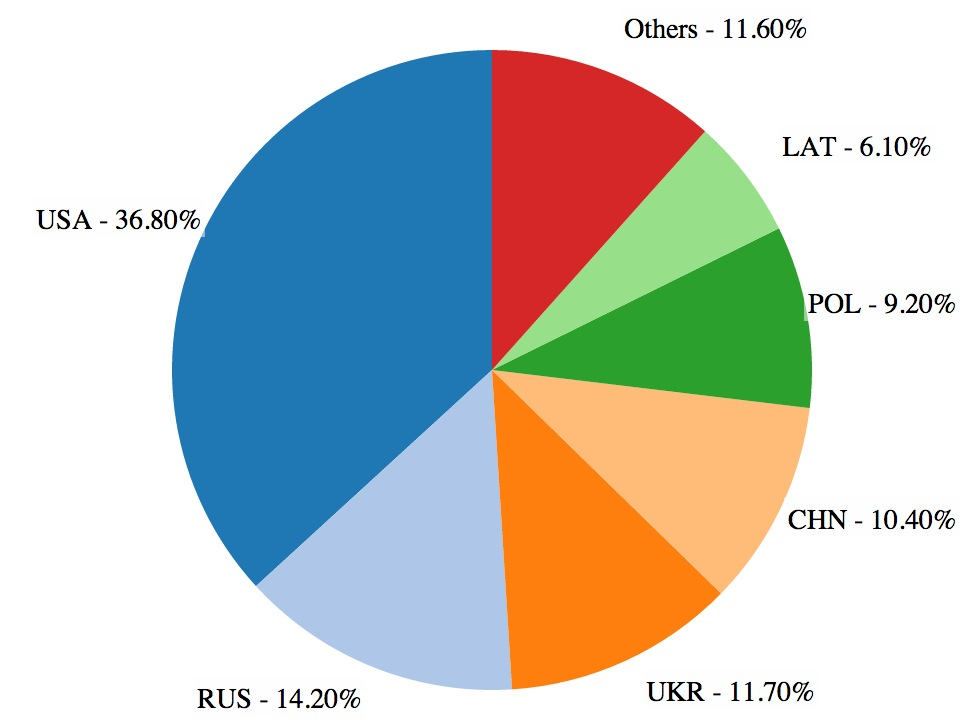
\includegraphics[width=0.8\textwidth]{Images/spamCountriesIP.jpg}}
\caption{Country provenance of IPs active on forum (message posting or registration).\label{fig:spamCountriesIP}}
\end{figure}

We tracked the geolocation of IP addresses responsible for registering users and posting to the forum. We identified the countries which are the most active on this category of rouge activity as the United States and Eastern Europe countries (mostly Russia, Ukraine, Poland, Latvia, Romania), as shown in Figure~\ref{fig:spamCountriesIP}. A total of 6687 distinct IP addresses were active on our forum (that is, posted at least one message or registered one or more accounts). Among these, 36.8\% were associated to locations in the US, while 51.6\% came from one of the cited Eastern European countries. The country coverage drastically changes if we consider only IP addresses that posted at least one message to the forum (ref Figure~\ref{fig:spamCountriesMessage}). In this case, IPs from the United States represent, alone, 62.3\% of all the IP addresses responsible for posting messages (Eastern Europe IPs in this case represent 21.2\% of the total), while we have much more variety in the number of different countries involved in the activity. This behaviour strongly suggests a country-related specialization in malicious activities, where a few number of attackers in few areas sell on the black market the results of their activities to foreign agents, who perform different activities.

\begin{figure}[tbh]
\centerline{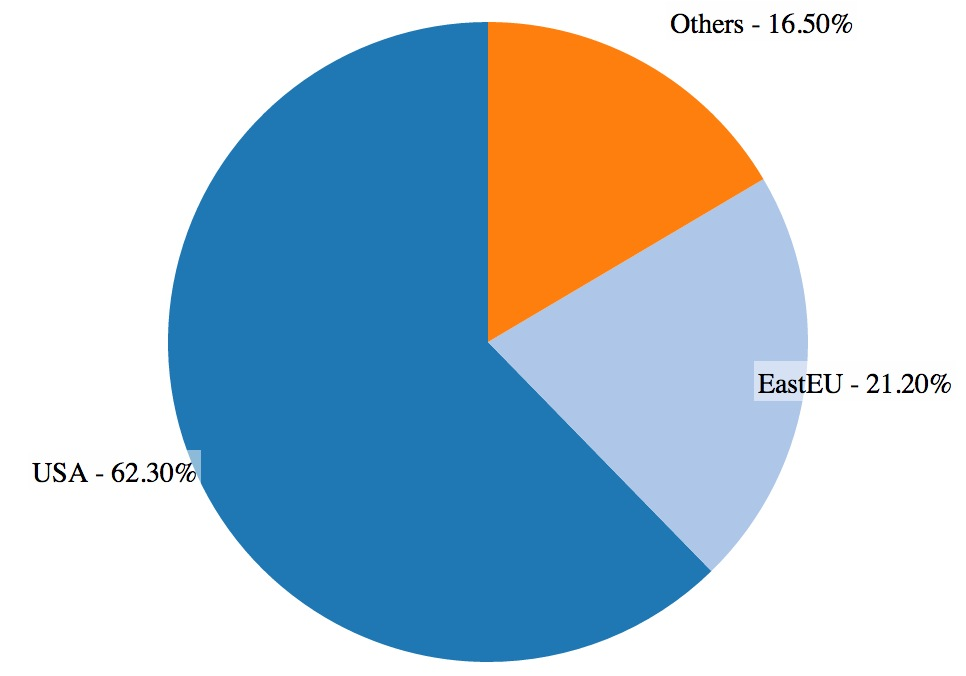
\includegraphics[width=0.8\textwidth]{Images/spamCountriesMessage.jpg}}
\caption{Country provenance of IPs posting at least one message.\label{fig:spamCountriesMessage}}
\end{figure}

Finally, we performed a simple categorization on all messages posted on the forum, based on the presence of certain keywords. This allowed us to quickly identify common spam topics and campaigns. Thanks to this method, we were able to automatically categorize 63,763 messages (93.5\% of the total).
As shown in Figure~\ref{fig:SpamCategory}, the trends we extracted from message topics reveal that the most common category is drugs (45.2\% of categorized messages, and showing peaks of 2000 messages per day), followed by search engine optimization (SEO, 17.4\%), electronics (13.5\%), adult content (7.9\%), and health care(5.2\%).
All links inserted in forum posts underwent an in-depth analysis using two automated, state-of-the-art tools for the detection of malicious web pages, namely Google Safe Browsing \cite{googleSafeBrowsing} and Wepawet \cite{wepaWet}. The detection results of these two tools show that, on the 221,423 URLs we extracted from forum posts, a small but not insignificant fraction (2248, roughly 1 out of 100) consisted in malicious or possibly harmful links.

\begin{figure}[tbh]
\centerline{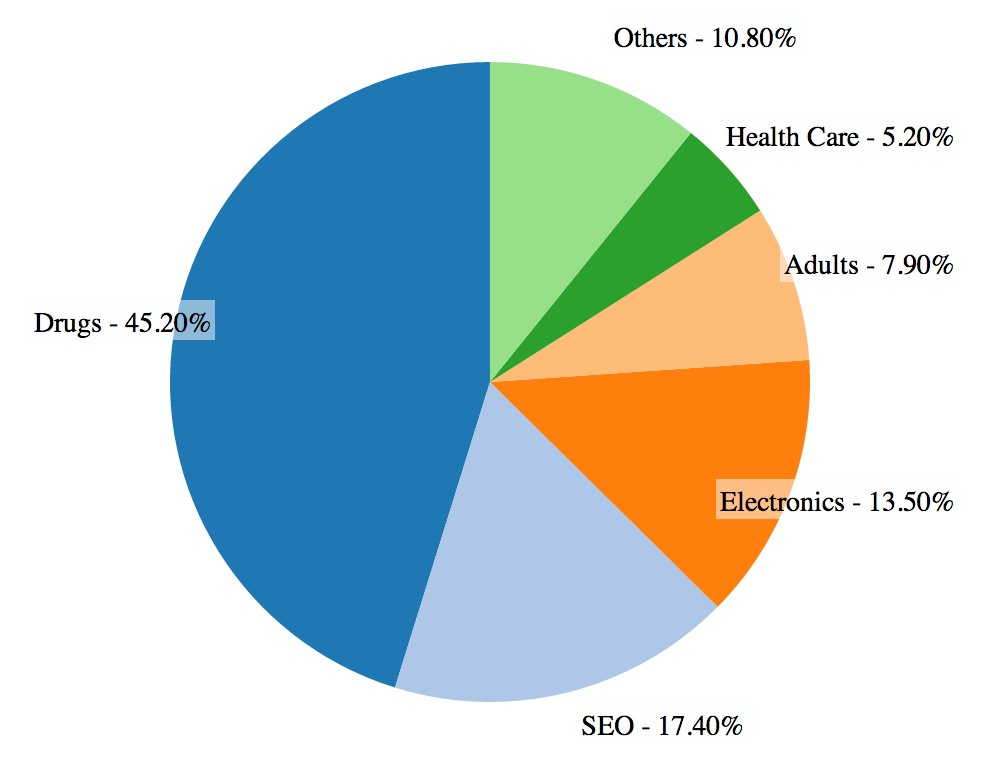
\includegraphics[width=0.8\textwidth]{Images/SpamCategory.jpg}}
\caption{Categories of spam messages.\label{fig:SpamCategory}}
\end{figure}

\subsection{Post-Exploitation}

The post-exploitation phase includes the analysis of the interaction between the attackers and the compromised machines. In our case, this is mostly done through the web shells installed during the exploitation phase or through the access to the public shells we pre-installed in our virtual machines.

The analysis of the post-exploitation phase deserves special attention since it is made of interactive sessions in which the attackers can issue arbitrary commands. However, these web shells do not have any notion of session: they just receive commands via HTTP requests and provide the responses in a state-less fashion. We decided to identify an ``interactive sessions'' every time a sequence of more than 3 commands is issued from the same IP and the idle time between consecutive commands is less than 5 minutes.
Over a total of 74,497 shell commands received, we registered 232 interactive sessions with an uploaded web shell and 8268 with one of our pre-installed shells. Because of the minimum number of commands threshold we imposed for the identification of a session only 52,368 shell commands have been included in a session. The majority of the commands not included in a session are single file uploads through one of our pre-installed web shells, mostly for defacement purposes.

The average session duration was of 5 minutes and 37 seconds, however, we registered 9 sessions lasting more than one hour each. The longest, in terms of commands issued to the system, was from a user in Saudi Arabia that sent 663 commands to the shell, including the manual editing of several files. Interestingly, one of the most common actions performed by users during an attack is the upload of a custom shell, even if the attacker broke into the system using a shell that was already available on the website. The reason for this behaviour is that attackers know that, with a high probability, shells already installed on a system will contain backdoors and most likely leak information to their owner. In addition to the 17 web shells supported by our tools, we also identified the HTTP patterns associated to the most common custom shells uploaded by the attackers, so that we could parse the majority of commands issued to them.
In 83\% of the cases, attackers tried to use at least one active command (uploading or editing a file, changing file permissions, creating files or directories, scanning hosts, killing a process, connecting to a database, sending emails, etc.). The remaining sessions were purely passive, with the attackers only browsing our system and downloading source and configuration files.
Finally, in 61\% of the sessions the attackers uploaded a new file, and in 50\% of them they tried to modify a file already on the machine (in 13\% of the cases to perform a defacement). Regarding individual commands, the most commonly executed were the ones related to listing and reading files and directories, followed by editing files, uploading files, running custom scripts/executables on the system, listing the processes running on the system, and downloading files.

During this phase most of the attackers created or uploaded a new file: as can be seen in Figure~\ref{fig:2ndStageAttack}, there is much more variety in the category of files uploaded, as during this stage the attackers is trying to accomplish a certain goal rather than just obtain an access to the machine. The results do not consider attacks where a web shell is uploaded, as we still consider this action to be a 1st stage attack.

\begin{figure}[tbh]
\centerline{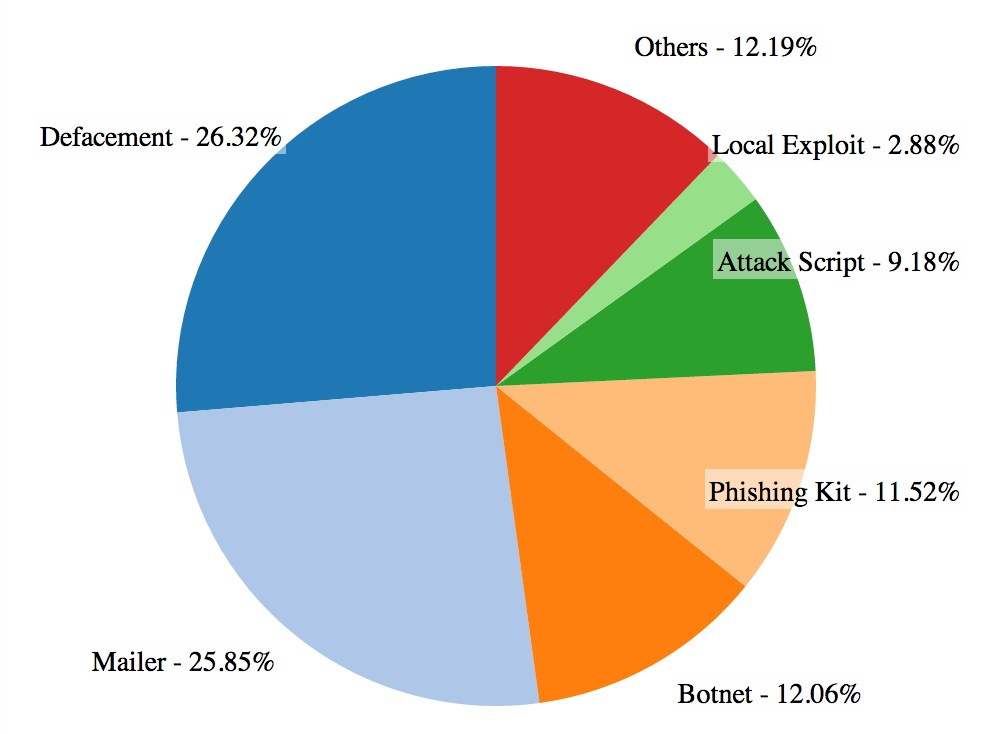
\includegraphics[width=0.8\textwidth]{Images/2ndStageAttack.jpg}}
\caption{2nd Stage Attack File Categorization\label{fig:2ndStageAttack}}
\end{figure}

It's evident how the variety of files is increased. In the next chapter we are going to explore in details attackers goals and single file categories, we provide here a first introduction to the various categories:

\begin{description}
\item[Defacement] The most common type of file uploaded, it's usually just an HTML document with the name of the attacker/team who performed the malicious activity;
\item[Mailer] A mailer is a script (usually written in PHP or Perl) for spamming purposes, it usually tries to read a list of e-mail addresses and sends the same message to each of them;
\item[Botnet] these scripts communicate with other machines for performing several tasks, transforming the hosting machine in a bot which receives and execute commands sent by others;
\item[Phishing Kit] it's a collection of HTML pages, images and CSS files, usually uploaded as a compressed archive, looking like a ``famous'' website in order to fool a victim to insert their credentials. The most common copied website is Paypal, followed by Visa and Bank Of America;
\item[Attack Scripts] This is a general category for including every script that is able to look for other websites and automatically exploit them. They usually accept a list of urls and, for each of them, they try to exploit a known vulnerability (like a vulnerable plugin for Joomla, etc);
\item[Local Exploits] This category relies with files that are trying to compromise the same machine they are running on, usually by means of privilege escalation.
\end{description}

Other categories include Uploaders, SQL dumpers, Malwares, Network Scanners, Drive-by Downloads, Flooder Scripts etc.

\section{Attackers Goals}

In this section we shift the focus from the way the attacks are performed to the motivation behind them. In other words, we try to understand what criminals do after they compromise a web application, and why. We discovered several goals attackers try to achieve after exploiting a machine: some of them are just looking for public recognition, some others are trying to create a botnet for profit, others are involved in spamming and phishing campaigns.

\begin{table}[tbh] % per piazzare la tabella t:top b:bottom h:here in ordine di preferenza; h è sconsigliato
\begin{center}
\begin{tabularx}{\textwidth}{|c|X|X|}
\hline
\textit{Category} & \textit{Unique Files} & \textit{Total Number Of Files} \\
\hline
Fake Download & 24 & 26 \\
Code Inclusion & 177 & 242 \\
Malicious Files Discovery & 216 & 217 \\
Java Applet & 221 & 225 \\
Drive-by Download & 284 & 310 \\
SQL dumper & 287 & 304 \\
Proxy & 335 & 353 \\
System Info Leaker & 341 & 397 \\
Mass Defacer & 356 & 683 \\
WebSearch Bot & 413 & 425 \\
Network Scanner & 420 & 445 \\
Malware & 475 & 492 \\
Documents & 516 & 518 \\
Uploader & 597 & 740 \\
Configuration Overloader & 656 & 713 \\
Backdoor & 703 & 728 \\
Bruteforcer Script & 1757 & 1959 \\
Local Exploit & 2033 & 2322 \\
Flooder Script & 2841 & 2952 \\
Attack Script (to other machines) & 3956 & 5064 \\
Botnet & 6878 & 7912 \\
Phishing Pack & 7445 & 16608 \\
Mailer & 11012 & 16324 \\
Defacement & 12698 & 13023 \\
Web Shell & 30522 & 38751 \\
\hline \hline
Total & 85163 & 111699 \\
\hline
\end{tabularx}
\caption{Summary of files Received.\label{tab:fileCategories}}
\end{center}
\end{table}

We analysed the files uploaded during the exploitation phase, and the ones created or modified during the post-exploitation phase. We normalized each file content, and we clustered them together according to their similarity, obtaining several clusters according to their ``purpose''. We identified a total of 25 categories, and the results are displayed in table~\ref{tab:fileCategories}. From the table we removed all broken files. The corresponding graphs (Figure~\ref{fig:graphCategories}) shows the distribution of files according to their percentage.

\begin{figure}
\centering
\begin{subfigure}{.5\textwidth}
  \centering
  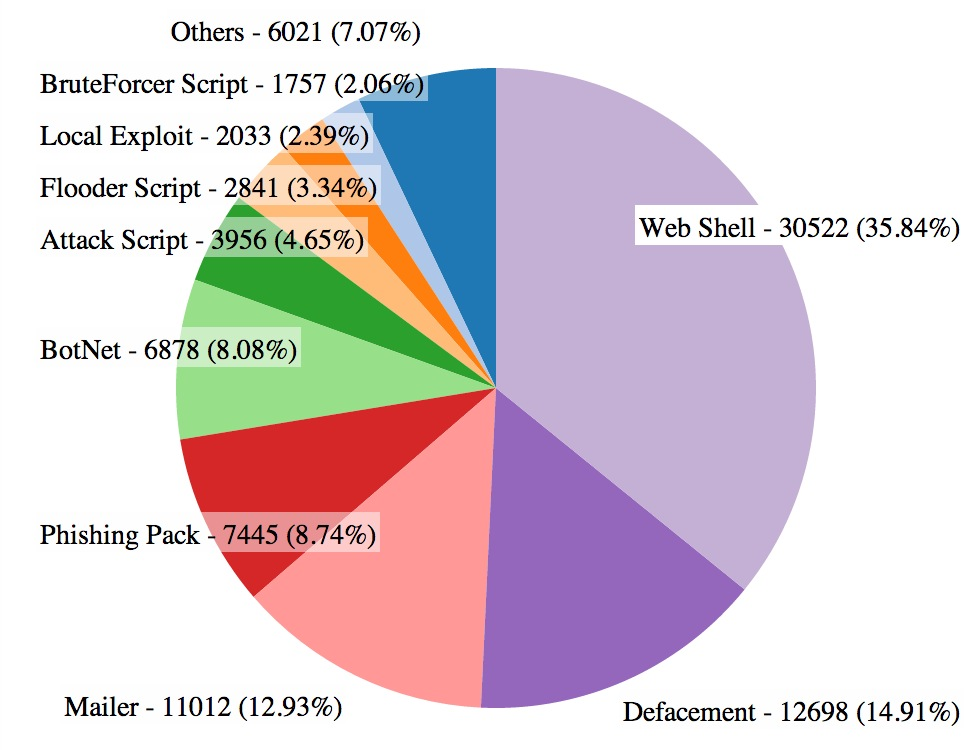
\includegraphics[width=1.0\linewidth]{Images/uniqueFiles.jpg}
  \caption{Unique Files Distribution}
  \label{fig:uniqueFileDistribution}
\end{subfigure}%
\begin{subfigure}{.5\textwidth}
  \centering
  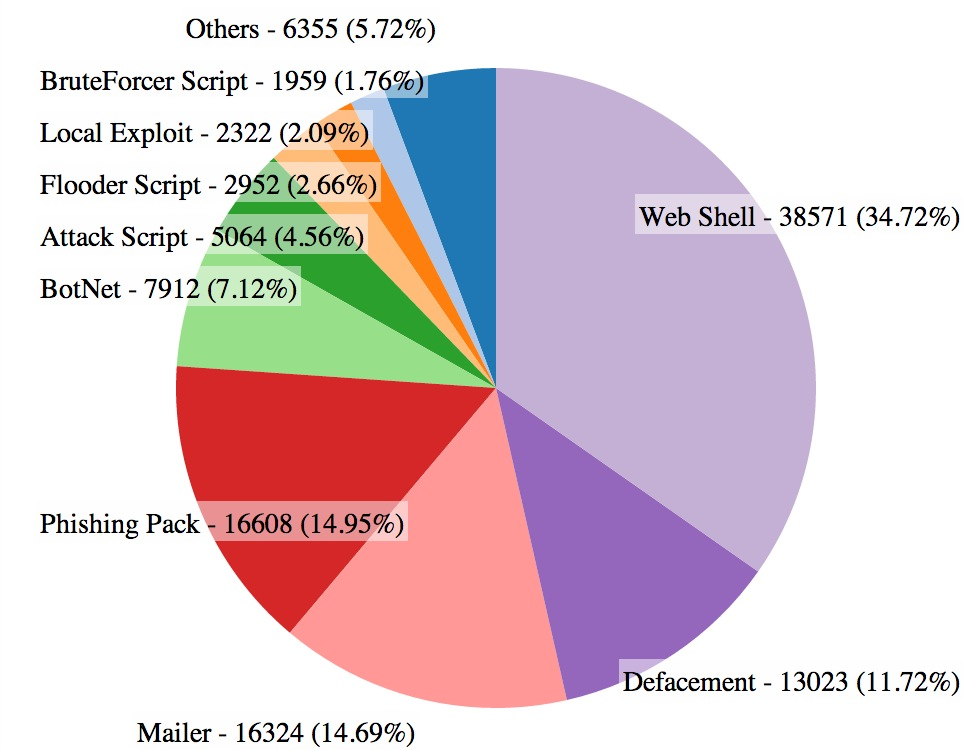
\includegraphics[width=1.0\linewidth]{Images/multipleFiles.jpg}
  \caption{Total Files Distribution}
  \label{fig:totalFilesDistribution}
\end{subfigure}
\caption{Categorization of files received}
\label{fig:graphCategories}
\end{figure}

For example, 2.3\% of the unique files we observed in our experiments were used to try to escalate the privileges on the compromised machine. This is different from saying that 2.3\% of the attackers tried to escalate the privileges of the machine. Unfortunately, linking the files to the attacks in which they were used is not always possible.

An interesting notice can be performed on the ratio between unique and total files received according to the category. Our results show how a few number of files are blindly reused by attackers, the only exceptions being phishing pack (which are obviously the same in most of the cases, the only thing changing is the script able to send logged credentials to the attacker, if present) and local exploits, because of the high complexity in creating exploits. From this we can conclude how, even if attackers are not professional programmers, most of them have some notions of programming languages, and can edit files in order to adapt them to their preferences.

In the rest of the section, we briefly explain each category, giving an example of file uploaded belonging to the category.

\subsection{Fake Download}

\begin{quote}
Number of Unique Files: 24\\
Number of Total Files: 26\\
Ratio (Unique/Total): 92.3\%
\end{quote}

This is the smallest category we have. In this category we include HTML pages offering to download a specific goodware which is actually a malware, often hosted on our honeypots. We consider this category as closely related to a phishing kit, as the page is often similar to a known webpage for software distribution (like FileHippo.com, softsonic.com etc.), but its purpose is different (malware distribution opposed to credential stealing).

It's worth to notice that in 6 cases the offered file is a tool for hacking purpose, like in the following example.
This file (ref. Figure~\ref{fig:graphCategories}) looks similar to the Download page of GeoGenSoft.com website, but, as can be seen, the software downloaded is coming from \url{http://www.gulfup.com/?8T4InX}. Our tests show the file which is actually downloaded after clicking on the link is a Zbot malware.

\begin{figure}[H]
\centerline{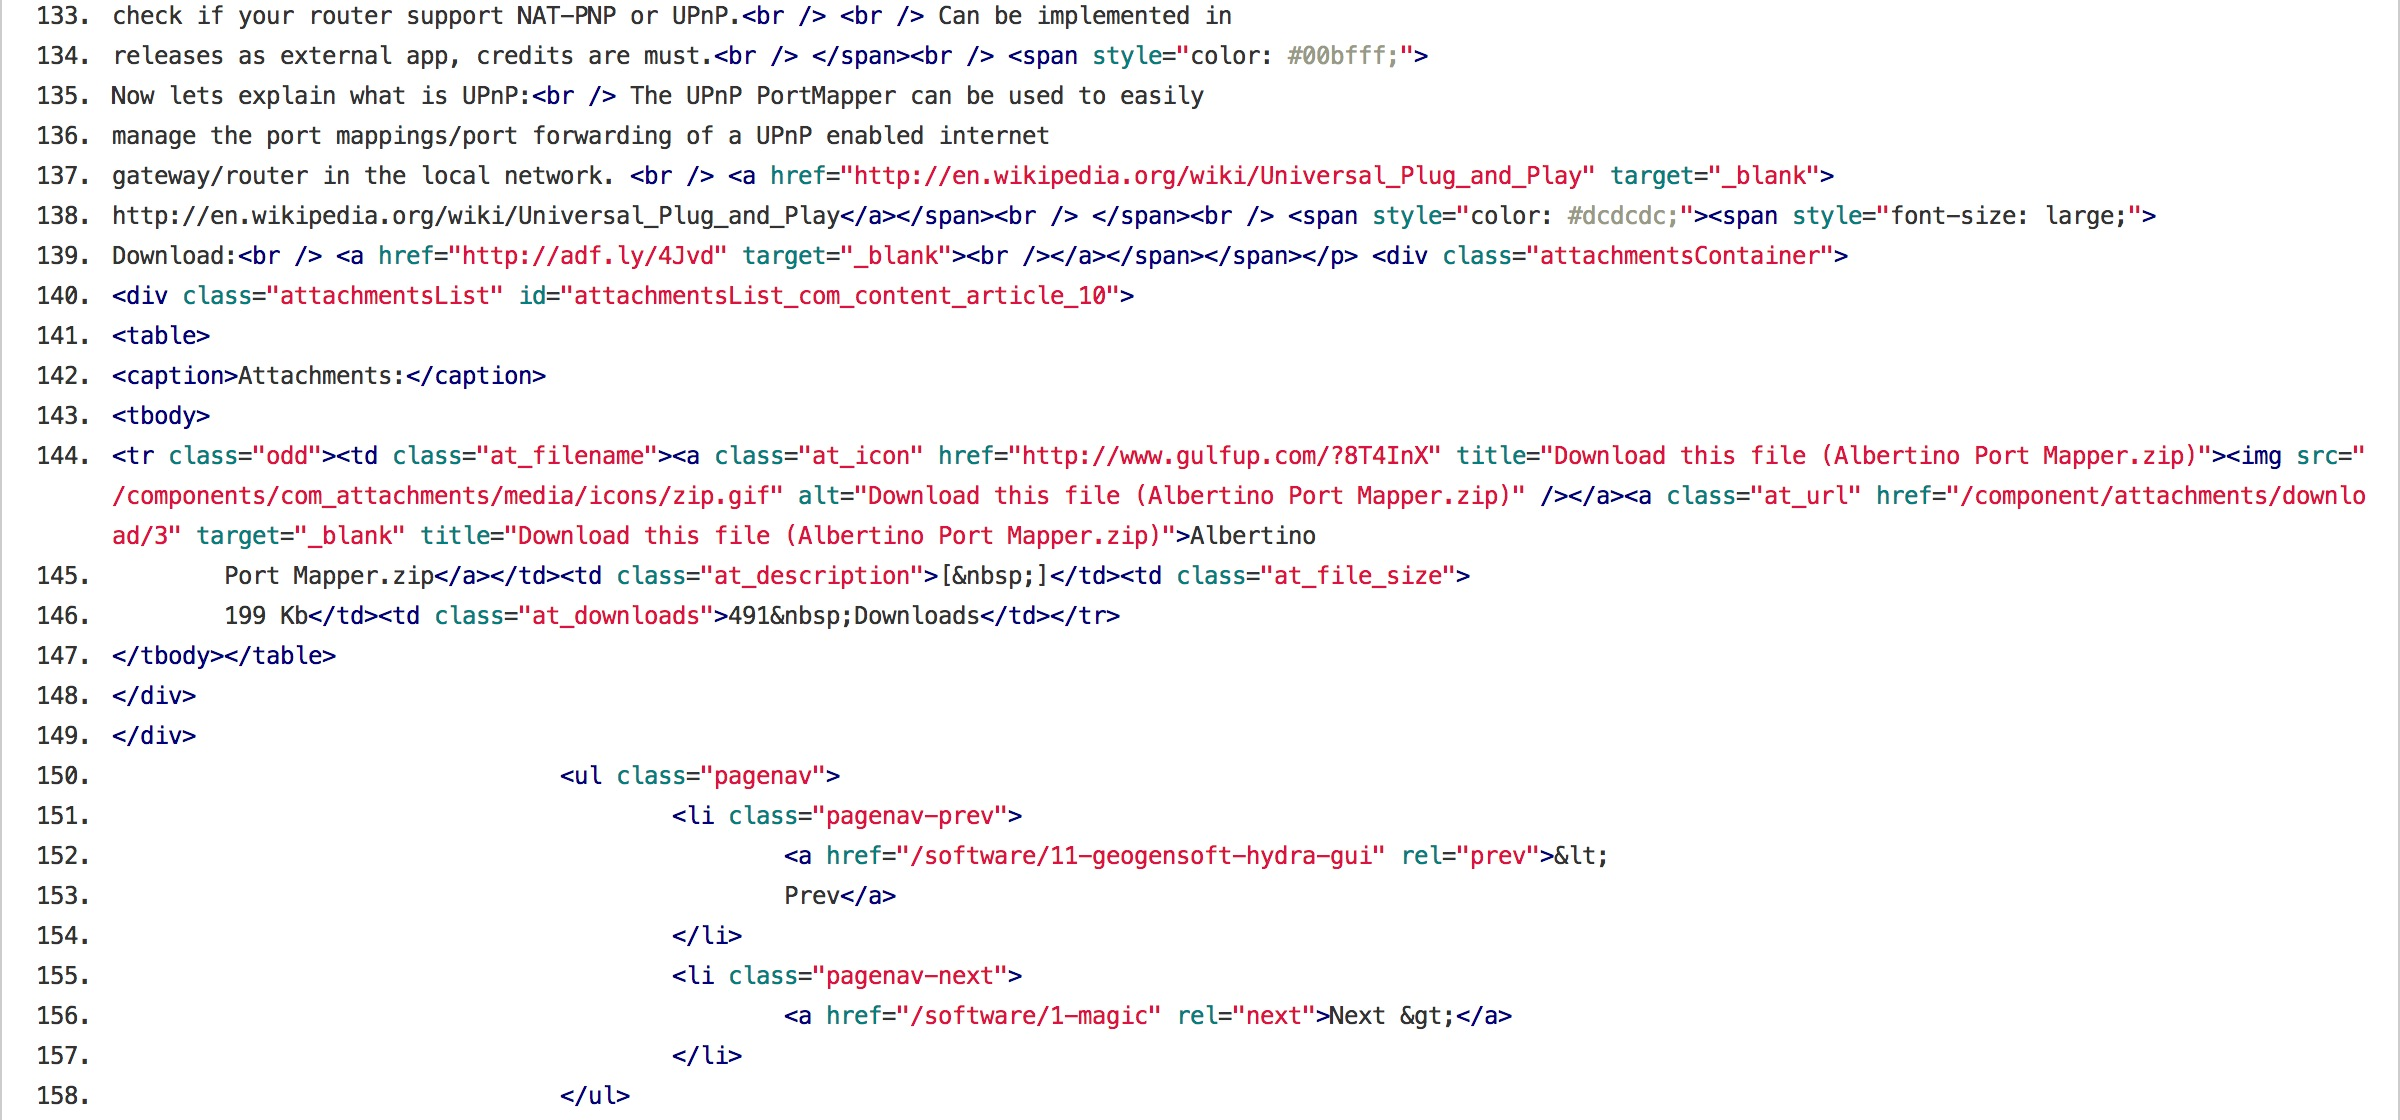
\includegraphics[width=0.8\textwidth]{Images/fakeDownload.jpg}}
\caption{Fake Download page Example (only the interesting part is displayed)\label{fig:fakeDownload}}
\end{figure}

\subsection{Code Inclusion}

\begin{quote}
Number of Unique Files: 177\\
Number of Total Files: 242\\
Ratio (Unique/Total): 73.1\%
\end{quote}

This is a category strictly related to drive-by download. The only difference is that files belonging to this category are ``similar'' to webpages that are actually hosted on our websites, while a drive-by download webpage can be a complete random page. By examining actions performed by the attacker before uploading the file, we discovered as he first tried to edit one of our webpages, but because of the impossibility to perform such an action, he simply copied one of our webpages and inserted its code into the latter one. The result is an HTML document (ref. Figure~\ref{fig:codeInclusion}) that is rendered as the original one, but with a malicious script injected. It's interesting to notice that we have quite a low ratio Unique/Total files. The motivation for this behaviour is that only the static website has been affected by this category of files, and the number of available pages on this web application is quite low. Furthermore, the number of different exploits available for modern browsers is quite low.
As example, we can look at \emph{wyoming.html}, an HTML document took from our static website with the addition, at the end of the page, of a VBScript for infecting the client with W32.Nimda worm.

 \begin{figure}[H]
\centerline{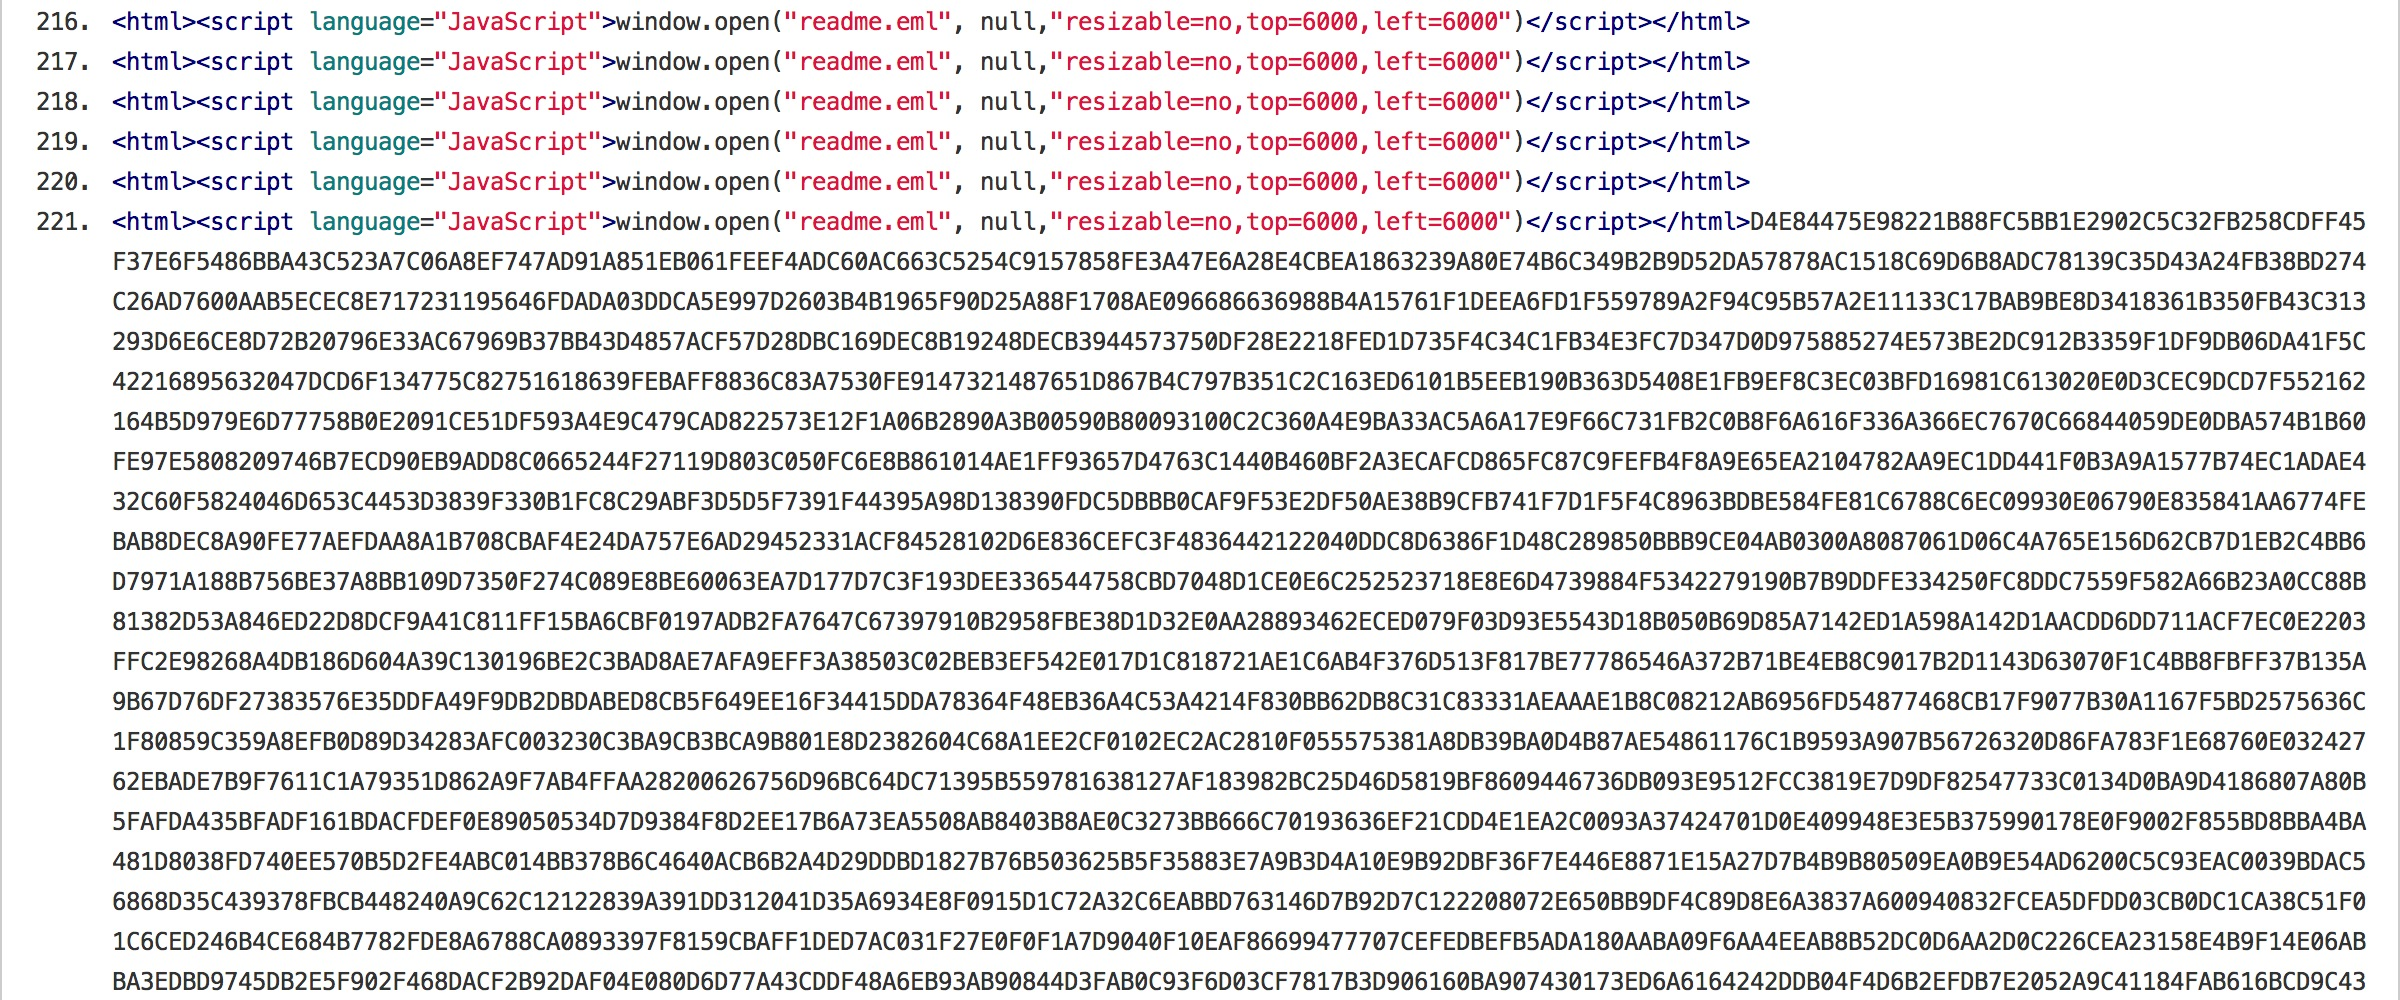
\includegraphics[width=0.8\textwidth]{Images/codeInclusion.jpg}}
\caption{Final part of wyoming.html Code Inclusion page (only the beginning of the VBScript is displayed)\label{fig:codeInclusion}}
\end{figure}

\subsection{Malicious Files Discovery}

\begin{quote}
Number of Unique Files: 216\\
Number of Total Files: 217\\
Ratio (Unique/Total): 99.5\%
\end{quote}

This category is quite uncommon, and there is no scientific literature describing it: this type of files are scanning the whole file-system, looking for files with suspicious names (like ``hacker.php'', ``shell.php'') or files containing suspicious patterns inside (like ``eval'' or ``base64\_decode'' calls, as shown in Figure~\ref{fig:maliciousFilesDiscovery}) and remove them. We noticed these files are removed from the system after they have been run, and that is probably the reason why no informations about this genre is available (we still recovered them directly from the Apache logs).

Almost every file belonging to this category uploaded on our machines is unique (the only file uploaded twice has the same source IP, with different targeted machines), making this category very interesting as we can conclude that the uploader is also the creator of the file.

 \begin{figure}[H]
\centerline{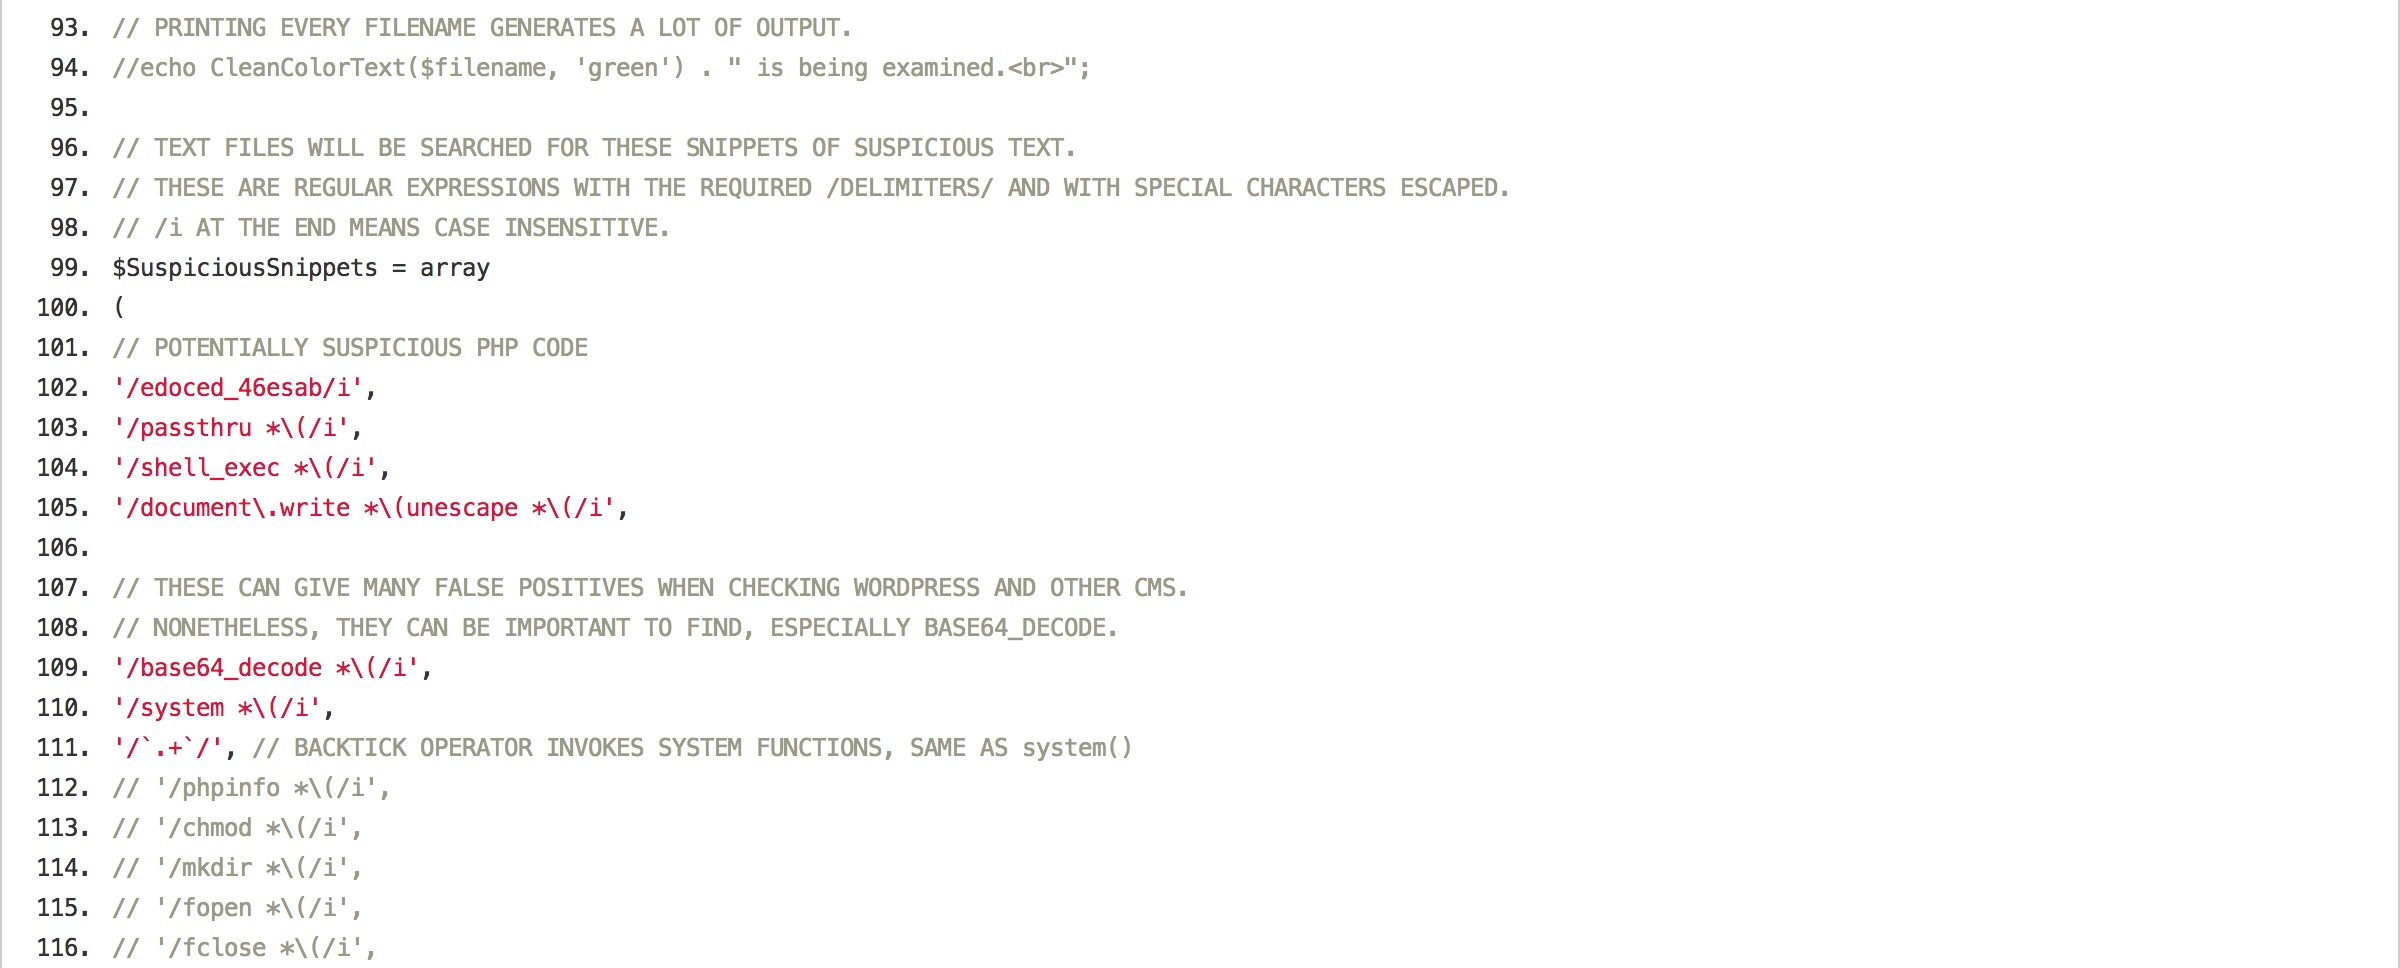
\includegraphics[width=0.8\textwidth]{Images/maliciousFilesDiscovery.jpg}}
\caption{Malicious Files Discovery example list of code regexes\label{fig:maliciousFilesDiscovery}}
\end{figure}

\subsection{Java Applet}

\begin{quote}
Number of Unique Files: 221\\
Number of Total Files: 225\\
Ratio (Unique/Total): 98.2\%
\end{quote}

A Java Applet is an application (usually small as it must be transferred during the loading of the page) delivered as byte-code. The code is executed in a Java Virtual Machine as a separate process with respect to the web browser. We found several examples of malicious applets, mostly exploiting the Java plugin in order to connect to a certain server and download malwares. We analysed in details Java applets by using JD-GUI \cite{jdgui}, an open source project which is able to deobfuscate Java byte-code and allowed us to examine the various classes.

An example of this category is shown in Figure~\ref{fig:javaApplet}. The code executed is exploiting a recent Java vulnerability (CVE-2013-0422 \cite{cveJava}), allowing Remote Code Execution outside the Sandbox. In particular, this Java Applet downloads a Zbot malware from an URL contained in a fake gif image, and then executes it. If successful, the client visiting the webpage becomes a bot inside one of the biggest botnets found in the wild.

 \begin{figure}[H]
\centerline{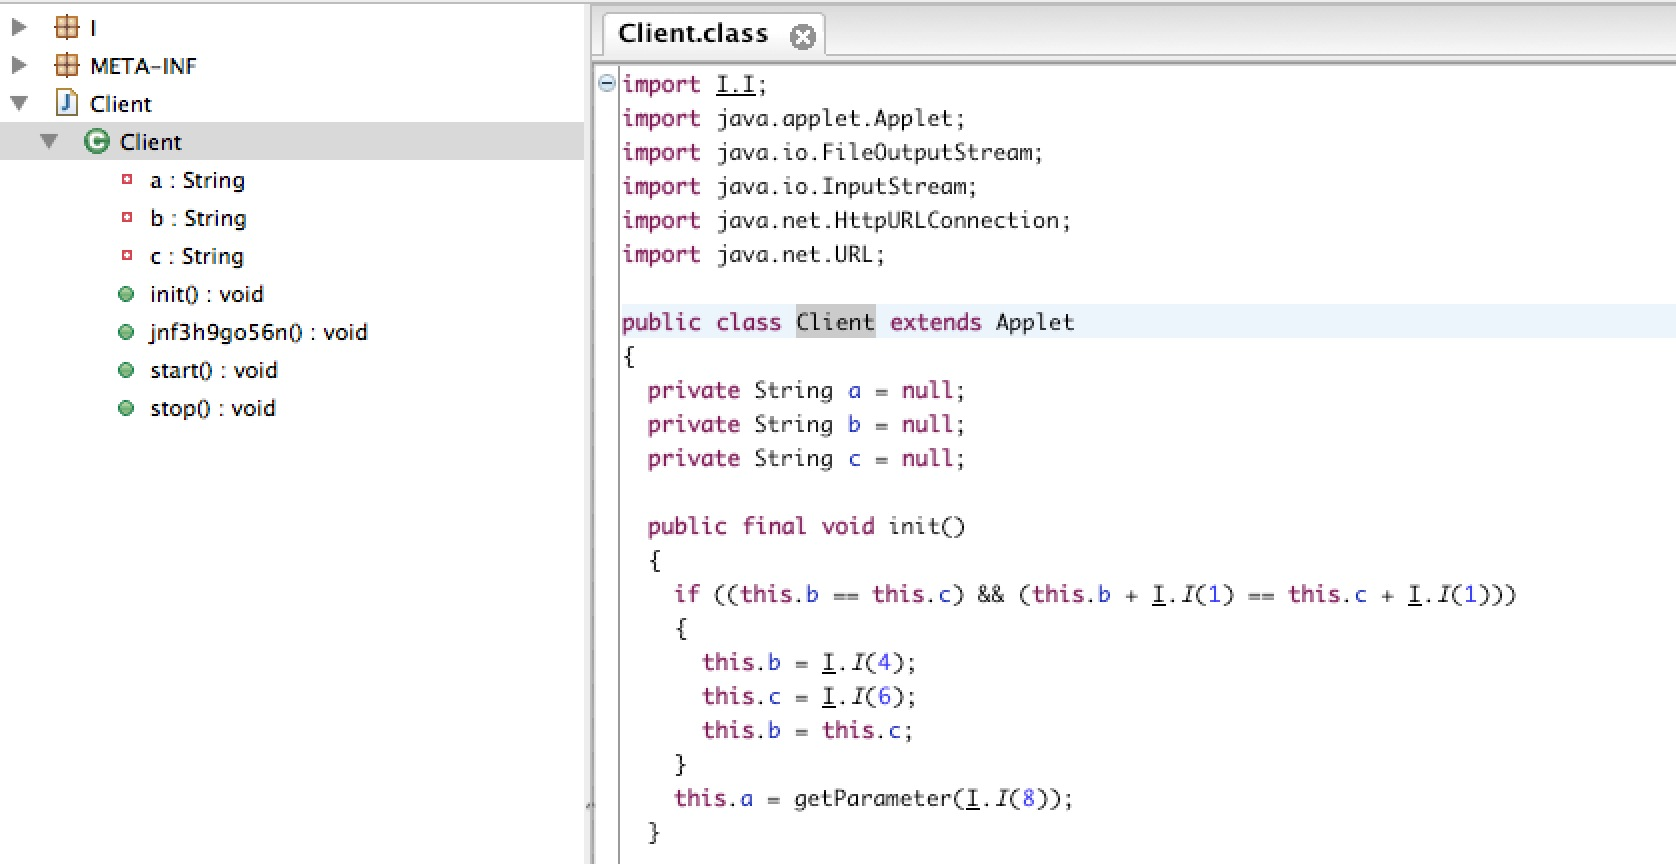
\includegraphics[width=0.8\textwidth]{Images/javaApplet.jpg}}
\caption{JD-GUI deobfuscation of a malicious Java Applet\label{fig:javaApplet}}
\end{figure}

\subsection{Drive-By Download}

\begin{quote}
Number of Unique Files: 284\\
Number of Total Files: 310\\
Ratio (Unique/Total): 91.6\%
\end{quote}

We categorized as Drive-By Download any webpage trying to exploit a vulnerability present in a web browser (or in a plugin) in order to perform a download (and possibly execution of downloaded content) without any notification to the user. It must be noticed that Java Applets are part of this category, but because of their relative frequency with respect to other types of drive-by downloads (Adobe exploits, VBScript) we preferred to separate them in another category. Code inclusion are also part of this category: the difference between the two is that while code inclusion refers to code injected into a page already present on our servers, Drive-By Downloads are separate HTML pages using our server for hosting purposes.
Most of the requests asking for this resource have their referrer set as a webmail or a popular social network (facebook, twitter). We can conclude that these requests are coming from victims who received a spam message and clicked on a link present inside them.

An example of Drive-By Downloads can be seen in Figure~\ref{fig:driveByDownload}. When opened, the page shows ``Intuit Market. Loading your order, please wait...''. In the mean time, an obfuscated script create an invisible iframe with src set to \url{http://twistedtarts.net/main.php?page=f231b7d2647c237a}. This page serves two exploits, one for Adobe PDF Reader plugin (CVE-2010-0188 \cite{CVE-2010-0188} and one for Microsoft Windows XP Help Center (CVE-2010-1885 \cite{CVE-2010-1885}). The first one, received as a PDF document, targets a Null Pointer Dereference Vulnerability present inside Adobe Acrobat 8.x up to 8.2.1 and 9.x up to 9.3.1, in order to provoke arbitrary code execution. In our case, the PDF document downloads and installs a Gamarue Worm on the victim. The second one is a relatively famous vulnerability, as it does not need any plugin for being run: the vulnerability relies on the fact that the MPC::HexToNum function in \emph{helpctr.exe} in Microsoft Windows Help and Support Center in Windows XP and Windows Server 2003 does not properly handle malformed escape sequences, which allows remote attackers to bypass the trusted documents whitelist (fromHCP option) and execute arbitrary commands via a crafted hcp:// URL, aka ``Help Center URL Validation Vulnerability.''. The purpose is the same as in the past exploit, downloading and executing a version of Gamarue Worm.

\begin{figure}[H]
\centerline{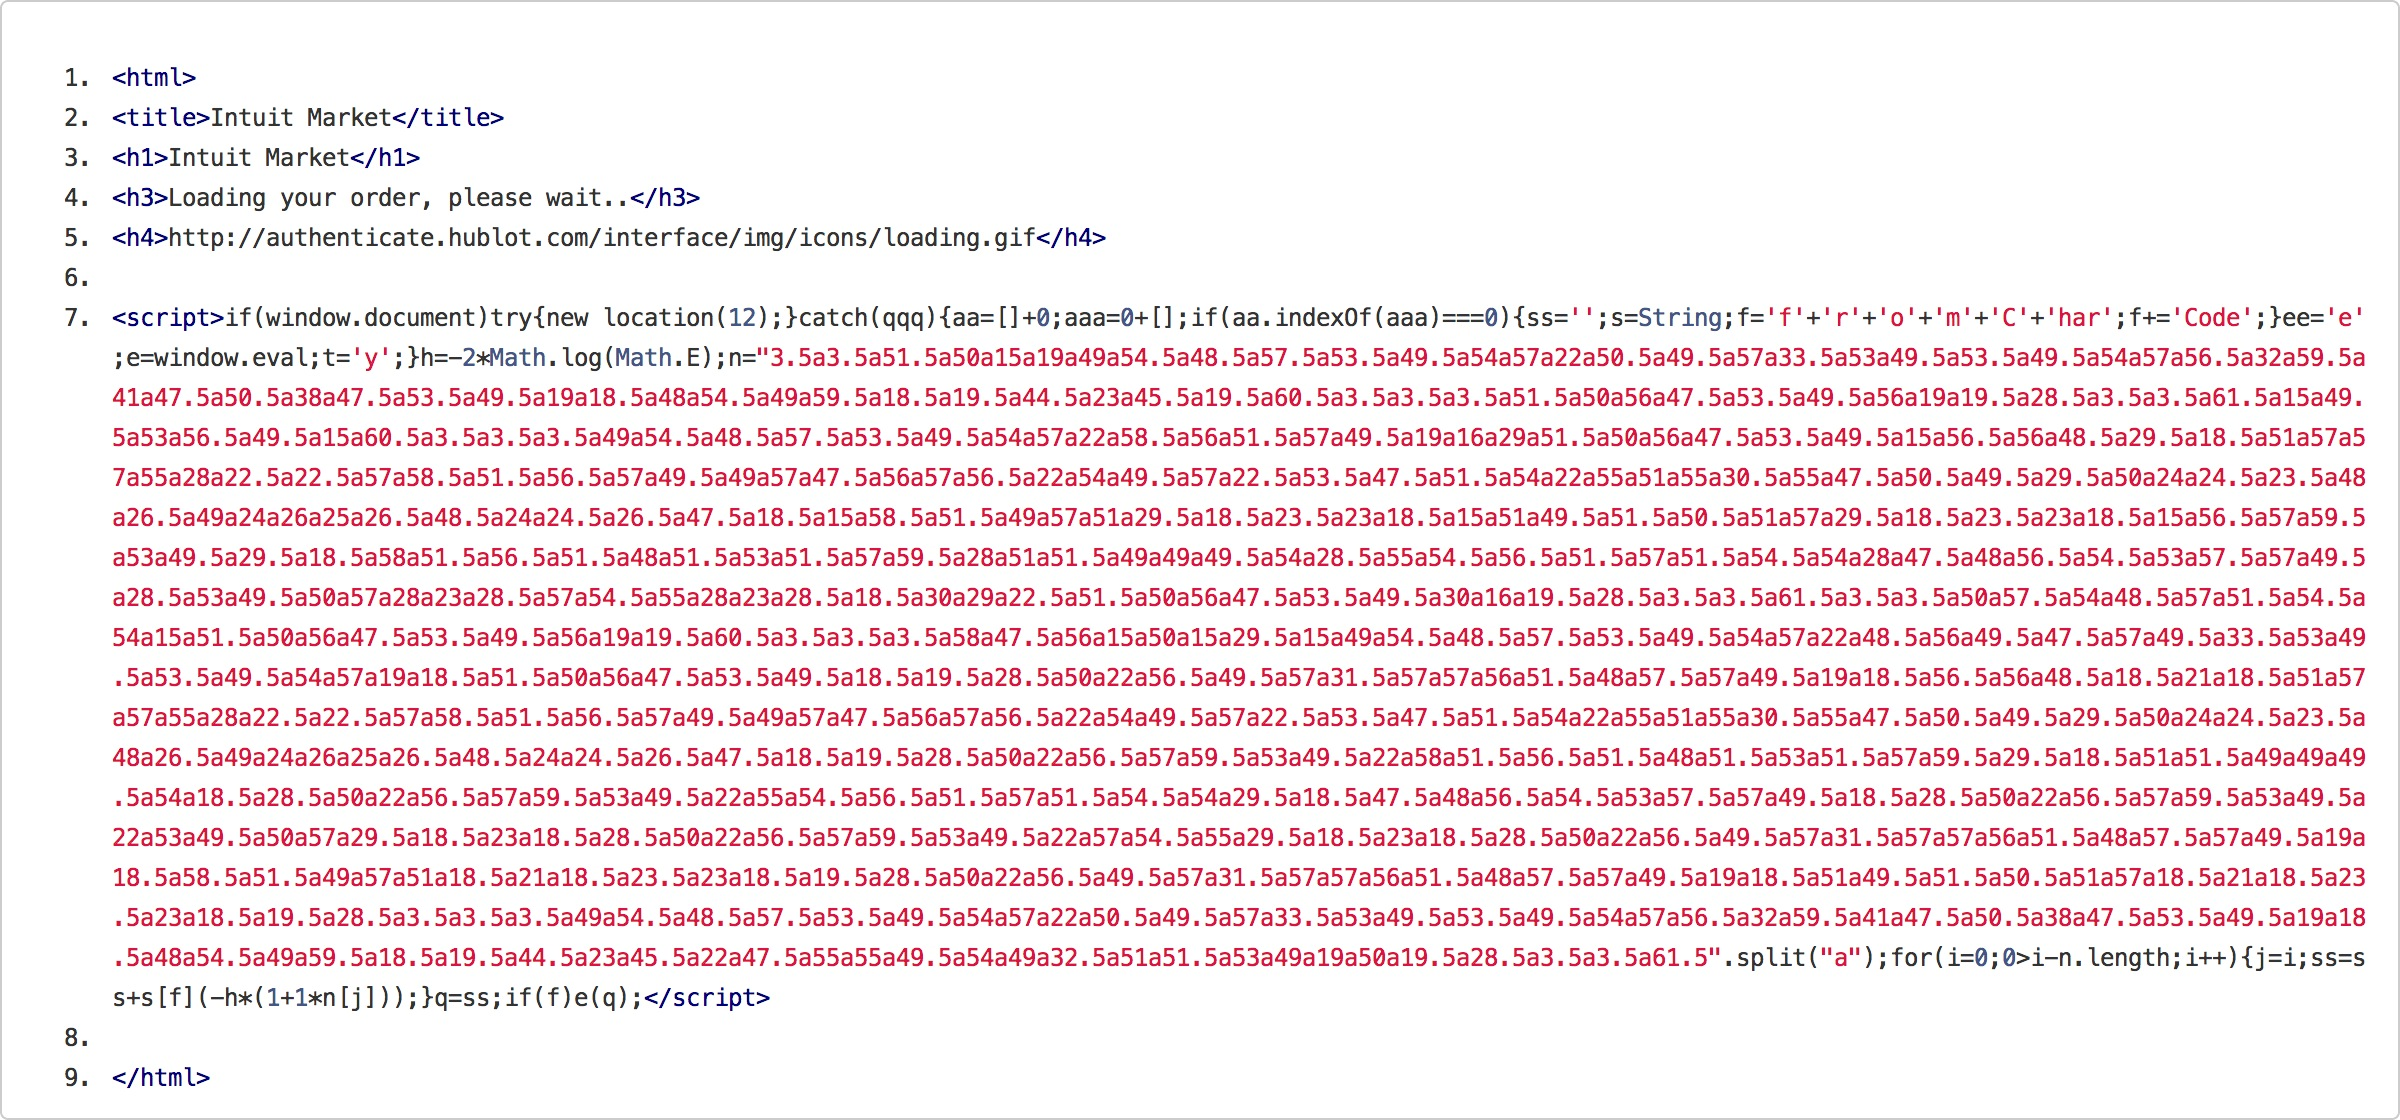
\includegraphics[width=0.8\textwidth]{Images/driveByDownload.jpg}}
\caption{Drive-By Download obfuscated Javascript\label{fig:driveByDownload}}
\end{figure}

\subsection{SQL Dumper}

\begin{quote}
Number of Unique Files: 287\\
Number of Total Files: 304\\
Ratio (Unique/Total): 94.4\%
\end{quote}

We include in this category every script which aims to dump an SQL database, storing the result in a file. We identified two types of files in this category: ones using user-provided username and password (through a GET/POST request) and ones relying on a word-list in order to find the right username and password to connect to the Database. Usually, this kind of script is able to dump different kinds of SQL databases, from MySQL to PostGresSQL. A specific peculiarity of this category is the quality of code: the functionality provided by this category is usually included in a Web Shell, and creating a script for this specific purpose denounce a higher professionalism in terms of code writing.

In the example provided in Figure~\ref{fig:SQLDumper} we show an example of SQL dumper: in particular, this piece of code is a general template for dumping a table from a database. It can be seen as the whole function contains error checks and pretty-printing possibility, confirming the programmer's ability in writing quality code.

\begin{figure}[H]
\centerline{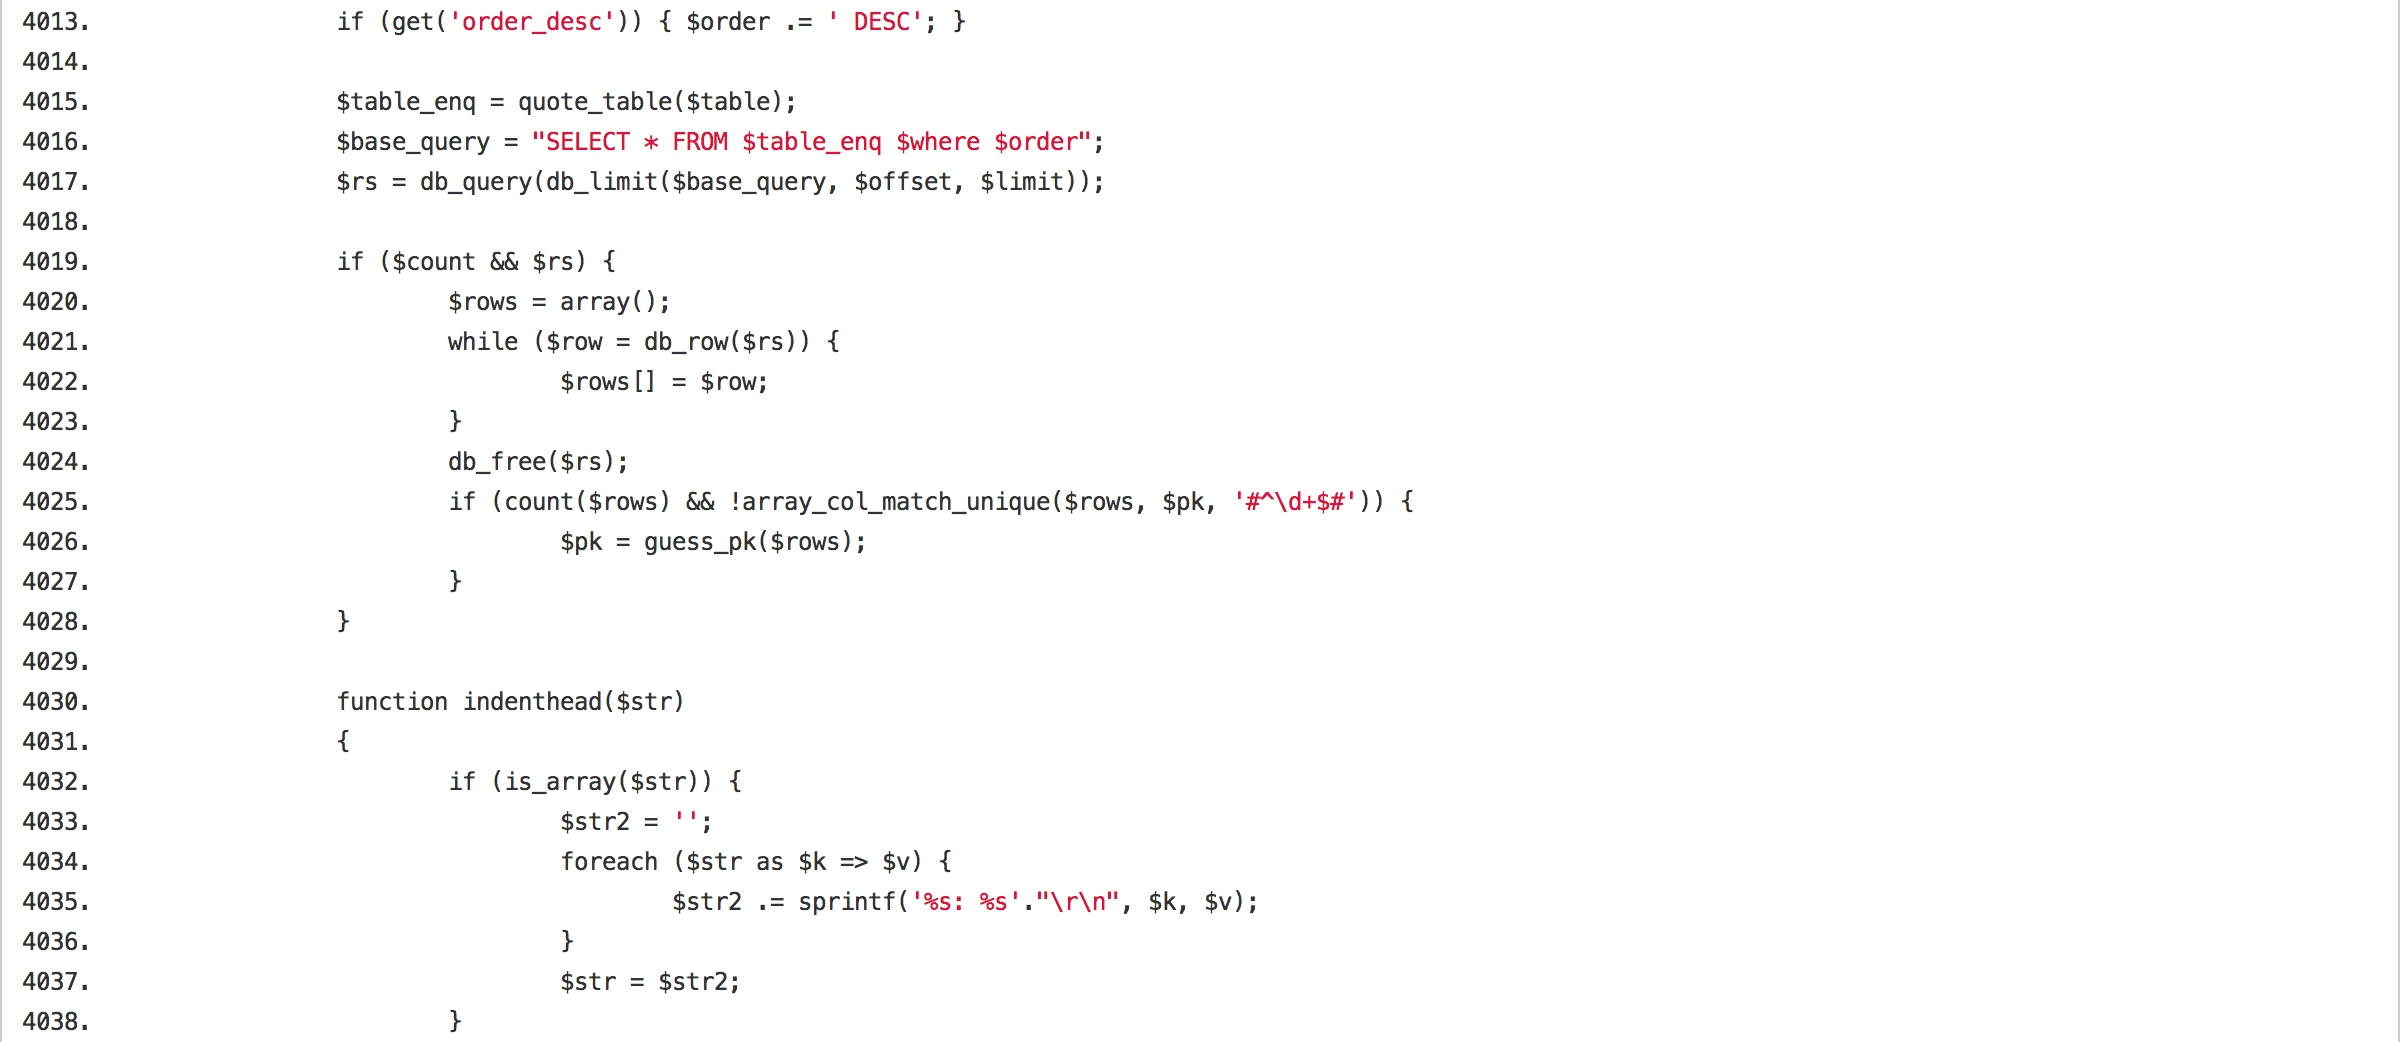
\includegraphics[width=0.8\textwidth]{Images/SQLDumper.jpg}}
\caption{SQL dumper table dumping function\label{fig:SQLDumper}}
\end{figure}

\subsection{Proxy}

\begin{quote}
Number of Unique Files: 335\\
Number of Total Files: 353\\
Ratio (Unique/Total): 94.9\%
\end{quote}

We defined a proxy as an application that acts as an intermediary for requests from clients seeking resources from other servers. A client connects to the proxy server, requesting some service, such as a file, connection, web page, or other resource available from a different server and the proxy server evaluates and execute the request, shadowing the real client. This system is often used by attackers to hide themselves during attacks, as the victim will see requests coming from the proxy (usually an already exploited machine) and not from the real criminal.
Most attackers use a botnet in order to perform their attacks while being in the shadows, while a proxy is more often used for manual attacks to other machines. As we didn't let the proxy run, we can't be sure about what attackers wanted to see while staying behind a proxy, but this is a study we could perform in the near future.

As shown in Figure~\ref{fig:Proxy}, most of the proxy scripts we received are working on crypted requests. In particular, the one shown in the example is using RC4 in order to decrypt the request coming from the attacker and to encrypt the response coming from the external server before connecting to the attacker.

In this category we also include simple scripts which are only performing a 301 redirection: we believe these scripts are often used during Phishing/Drive-By Download attacks, in order to make it harder for the defence to track bad servers.

\begin{figure}[H]
\centerline{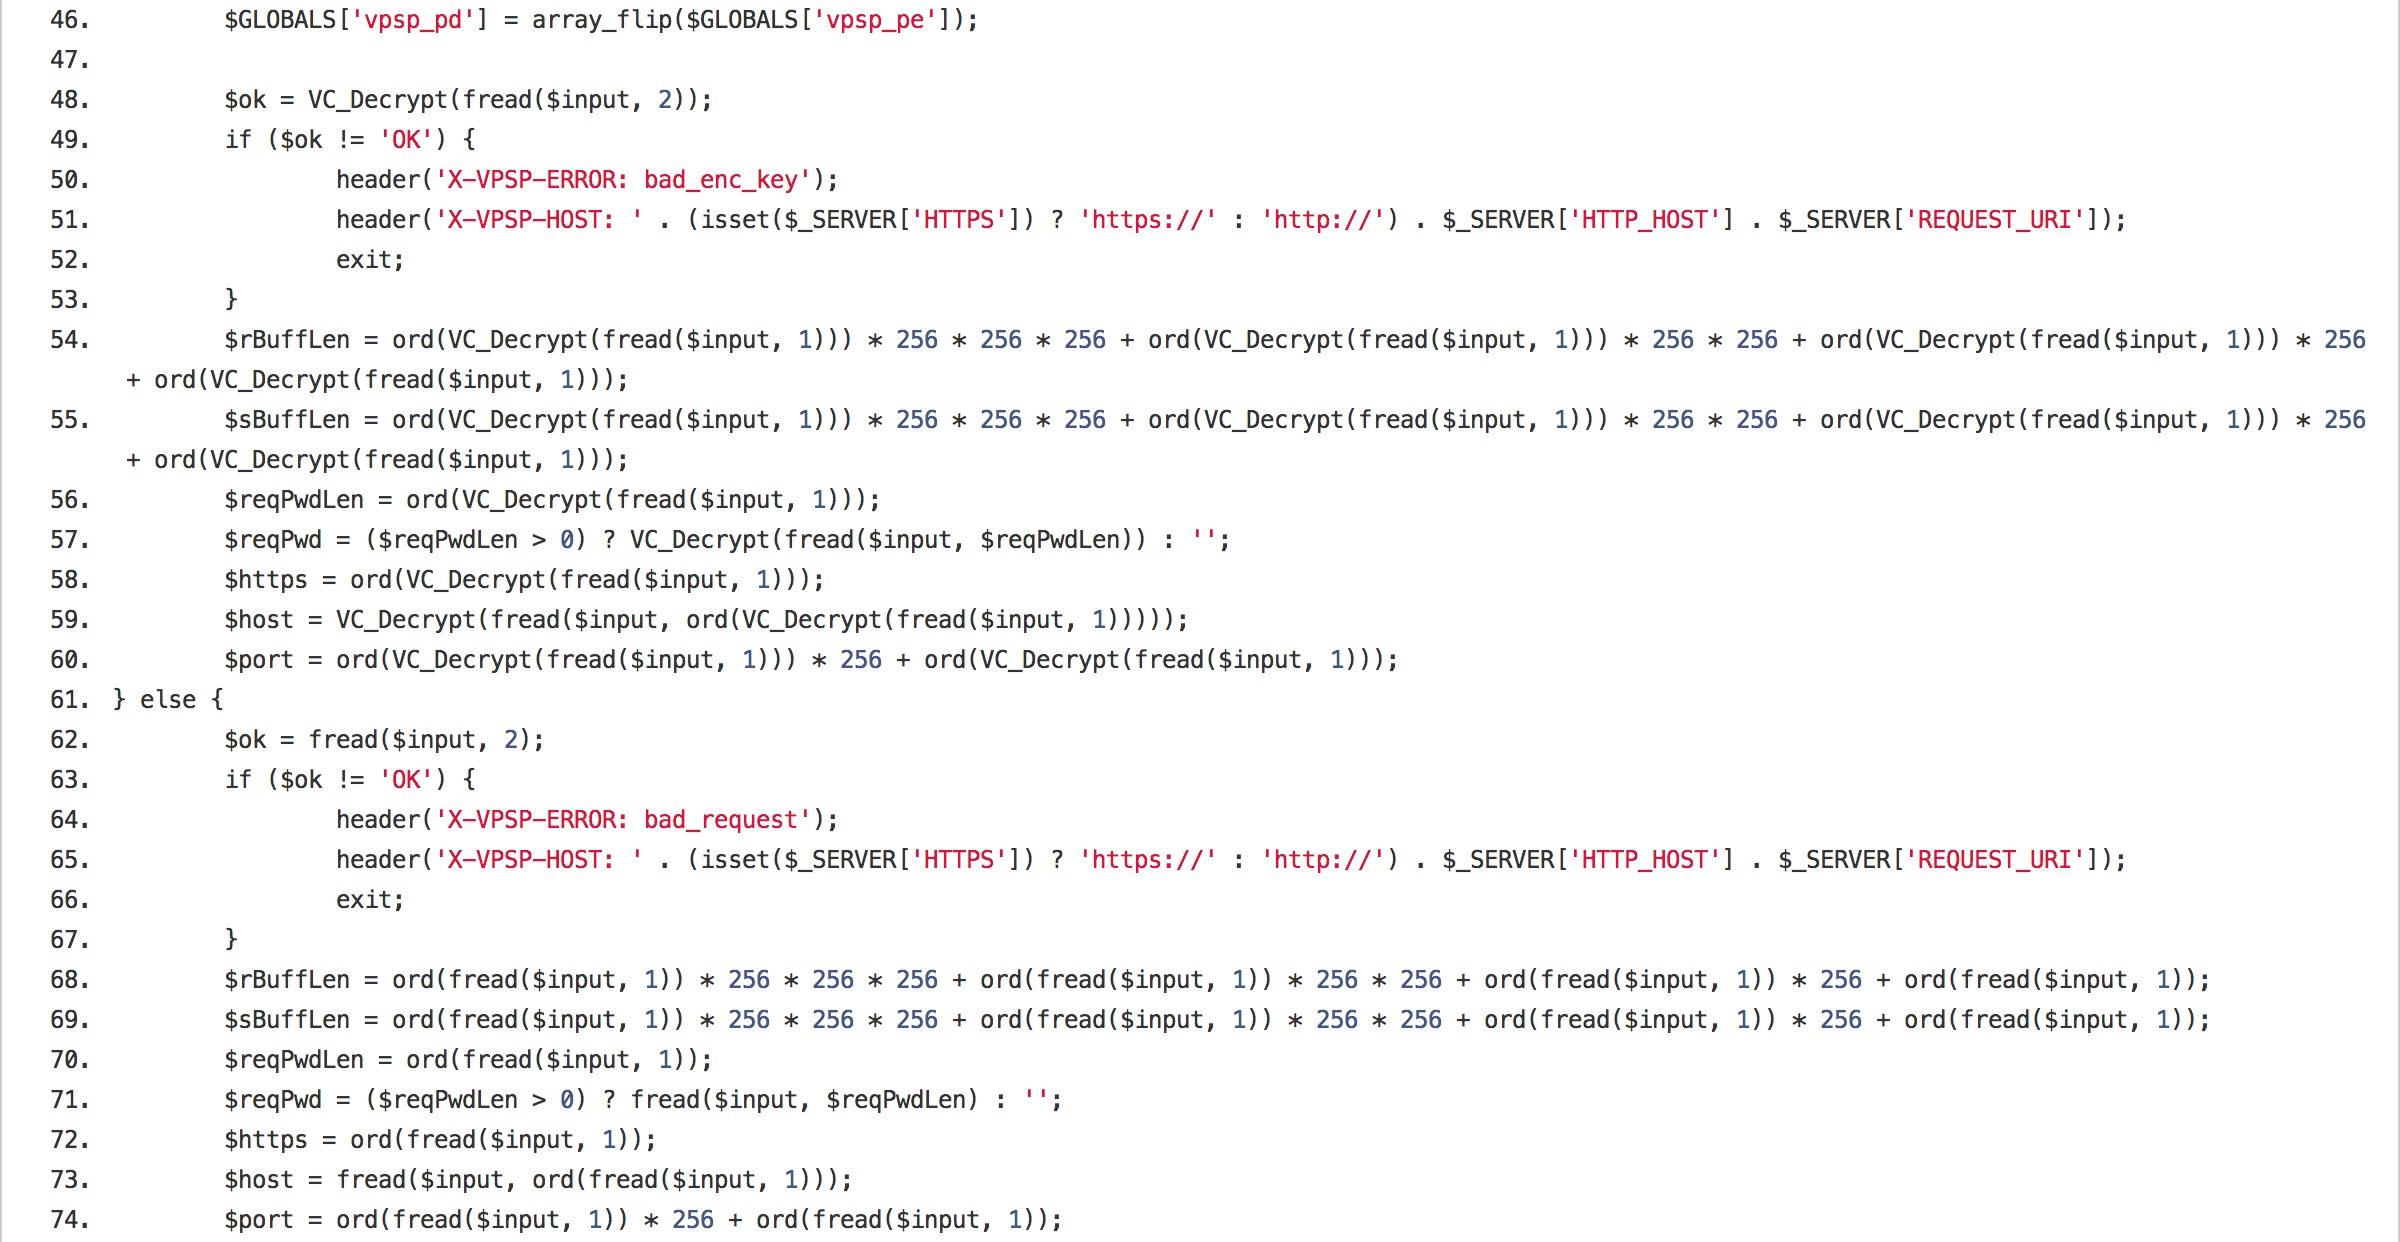
\includegraphics[width=0.8\textwidth]{Images/Proxy.jpg}}
\caption{Function inside proxy aimed for decrypting the request coming from the attacker\label{fig:Proxy}}
\end{figure}

\subsection{System Info Leaker}

\begin{quote}
Number of Unique Files: 341\\
Number of Total Files: 397\\
Ratio (Unique/Total): 85.9\%
\end{quote}

We defined as a generic System Info Leaker any script able to extract configuration informations from the server. That means reading /etc/hosts, /etc/passwd, .htaccess, and similar files and reporting these informations to the attacker. Another kind of files included in this category are scripts compressing the whole /var/www/ folder and sending it to the attacker.
This category is strictly related to SQL Dumper: both of them, in fact, provide a functionality that is usually included in a web shell, and separation of functionalities can be considered as one of the fundamental steps for obtaining reliable and maintainable code.

The example shown in Figure~\ref{fig:SysInfoLeaker} is a Perl script (Perl is a programming language which is often used by attackers) able to compress a list of files in a single archive and make it available for download. This technique is often used by attackers in order to download several informations in a short amount of time, discovering both configuration informations (domains, users, groups etc.) and eventual private files (users often have a password file where they store database credentials).

\begin{figure}[H]
\centerline{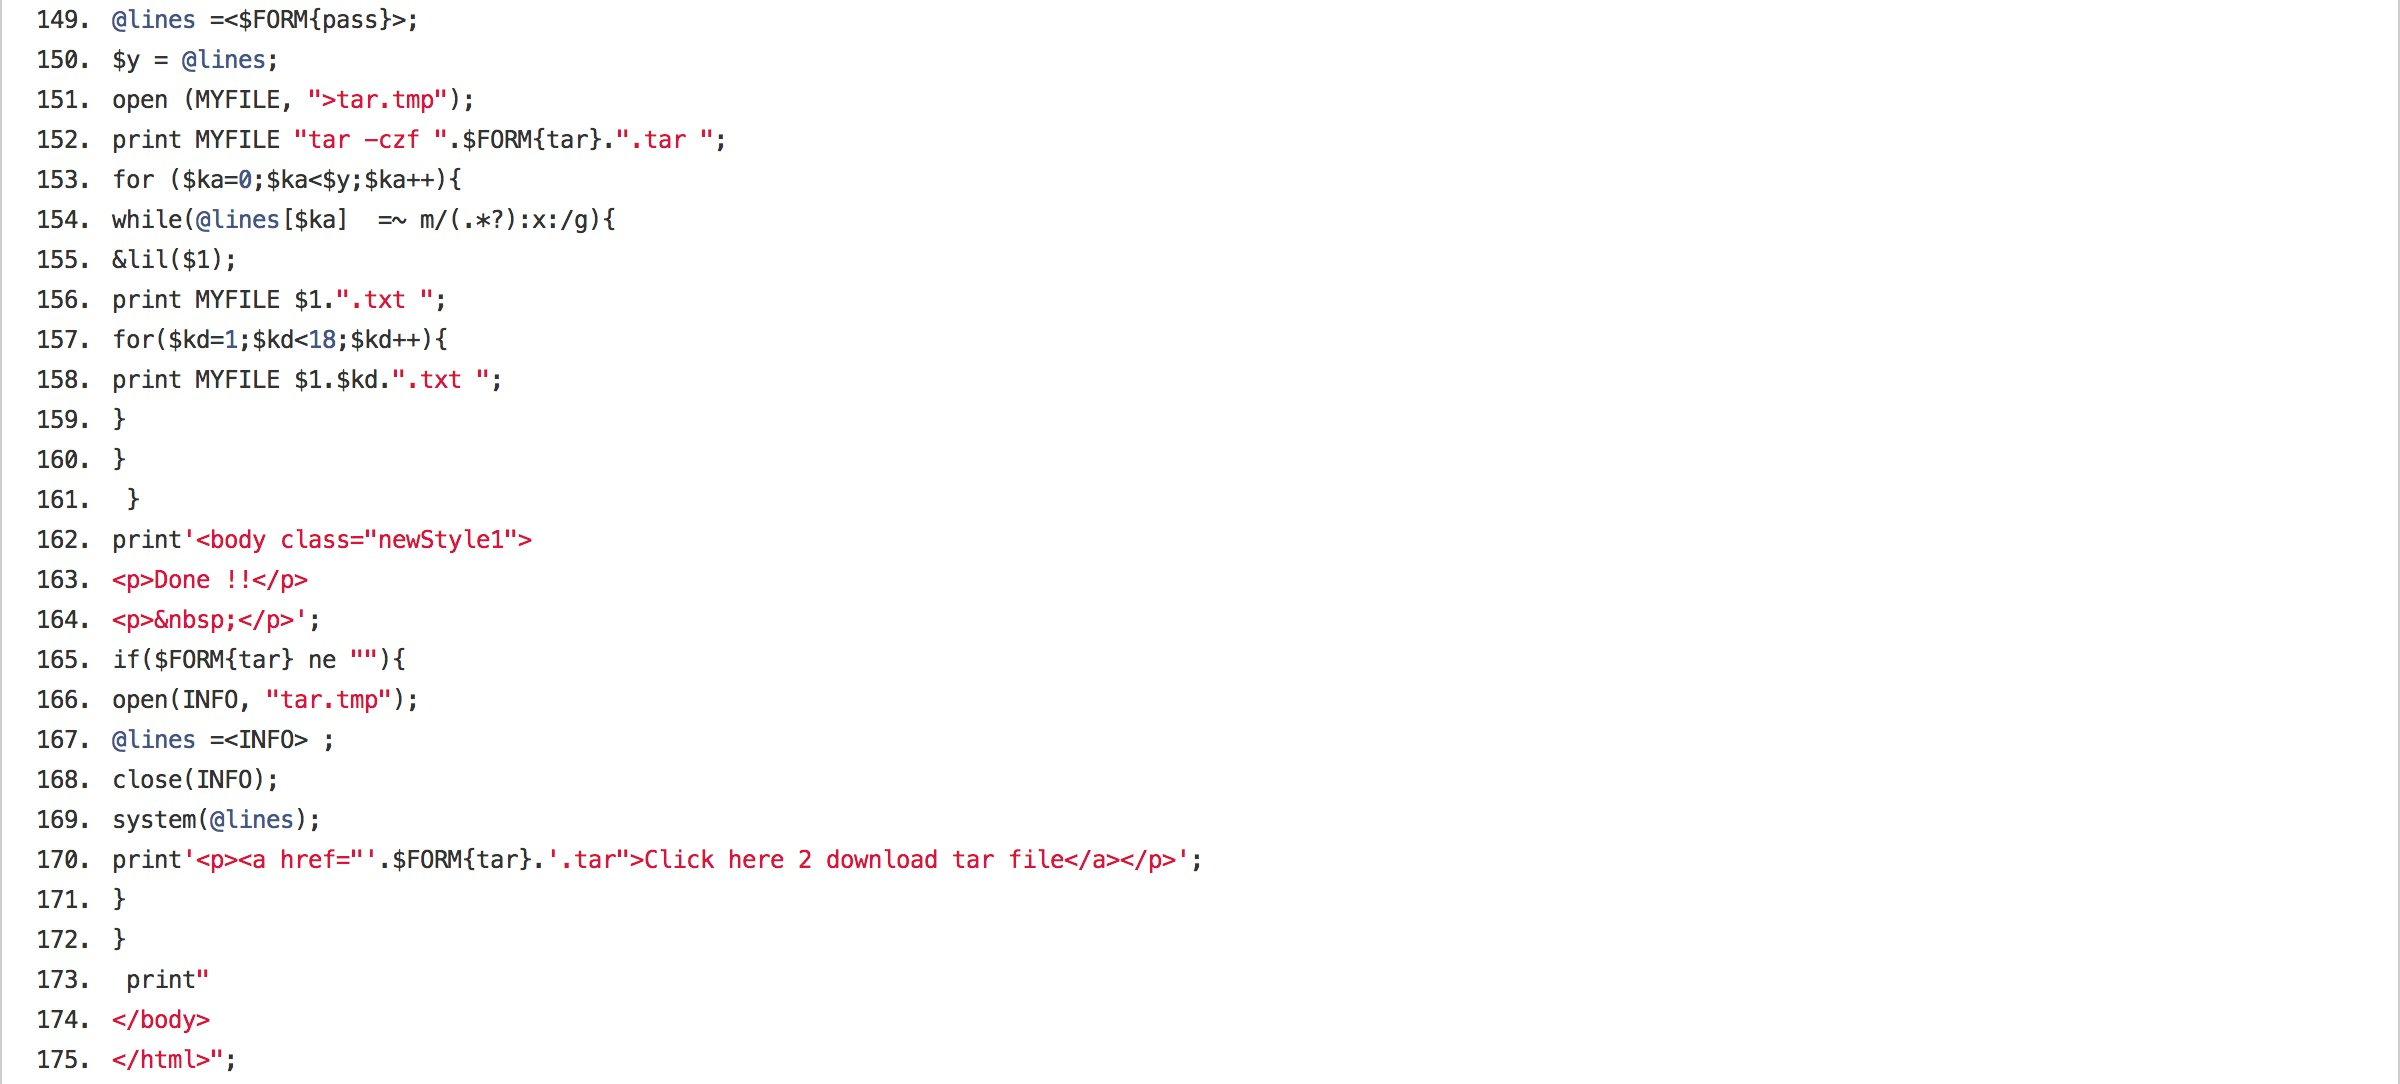
\includegraphics[width=0.8\textwidth]{Images/SysInfoLeaker.jpg}}
\caption{System Info Leaker Compressing function\label{fig:SysInfoLeaker}}
\end{figure}

\subsection{Mass Defacer}

\begin{quote}
Number of Unique Files: 356\\
Number of Total Files: 683\\
Ratio (Unique/Total): 52.1\%
\end{quote}

A Mass Defacer is a tool (usually a PHP script) an attacker can use while performing a defacement attack: a defacement is an attack that aims to change the visual appearance of a website. A mass defacer generally works on two main directions: on one side, it overloads every single page on the website with a symbolic link to a single page, on the other hand it writes this single page, which is a usual defacement page.

This category is loosely related to the System Info Leaker one, and files often belong to both categories, as before setting up a mass defacement the attacker has to understand the topology of the website. The relatively low percentage of Unique/Total files ratio allows us to conclude that this kind of files have been developed by groups of attackers who share their scripts among each other, so that each member can then use the same version of the file in order to perform the attack.

In Figure~\ref{fig:massDefacement} we show a variation from the common behaviour: this script, in fact, after listing all files present on the web server does not create symbolic links but overwrite directly all pages with the defacement one. Of course this operation fails on our machines as all our files do not have write permissions.

\begin{figure}[H]
\centerline{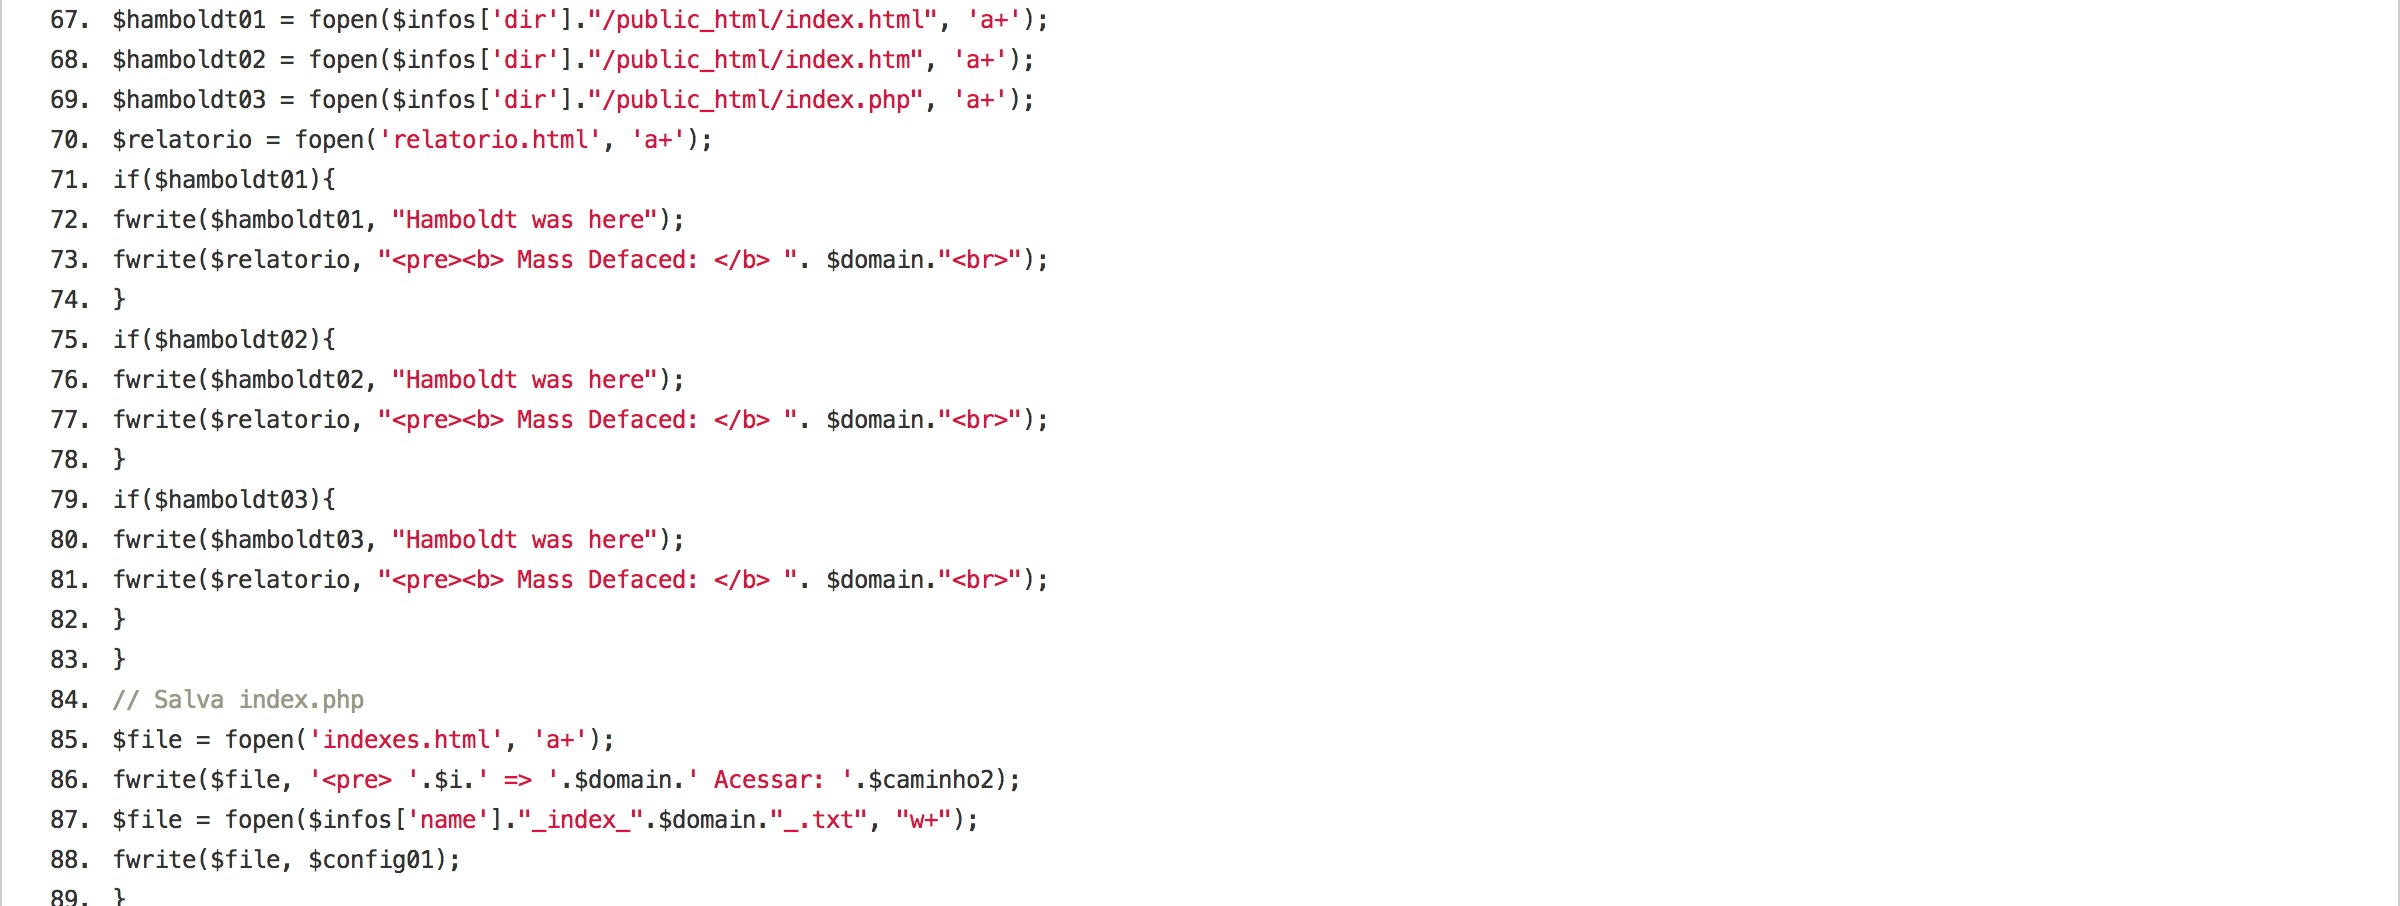
\includegraphics[width=0.8\textwidth]{Images/massDefacement.jpg}}
\caption{System Info Leaker Compressing function\label{fig:massDefacement}}
\end{figure}

\subsection{Web Search Bot}

\begin{quote}
Number of Unique Files: 413\\
Number of Total Files: 425\\
Ratio (Unique/Total): 97.2\%
\end{quote}

Reconnaissance is the first phase of an attack. During this phase, criminals often use a bot in order to automatically perform queries toward common search engines, looking for particular dorks in order to find exploitable websites. Because of the limit in the number of queries per IP every search engine allows, attackers often try to parallelize the process by performing queries from different machines, and using an already exploited one seems to be a common practice.

The most targeted web search engines used for this activity are Google, Bing, Yandex and Yahoo. Queries are often embedded directly in the scripts (hardcoded), and results are usually displayed as an HTML page or sent via e-mail to the attacker.

An interesting example of Web Search Bot is displayed in Figure~\ref{fig:webSearchBot}: this particular Bot does not rely on common dorks for finding vulnerable versions of CMSs, but rather tries to look for web shells that have been crawled by the Search Engine. This practice is commonly used by attackers for finding easy target during SEO Campaigns or Mass Defacement, as the exploit has already been performed by somebody else and they just have to upload their files using the already present shell.

\begin{figure}[H]
\centerline{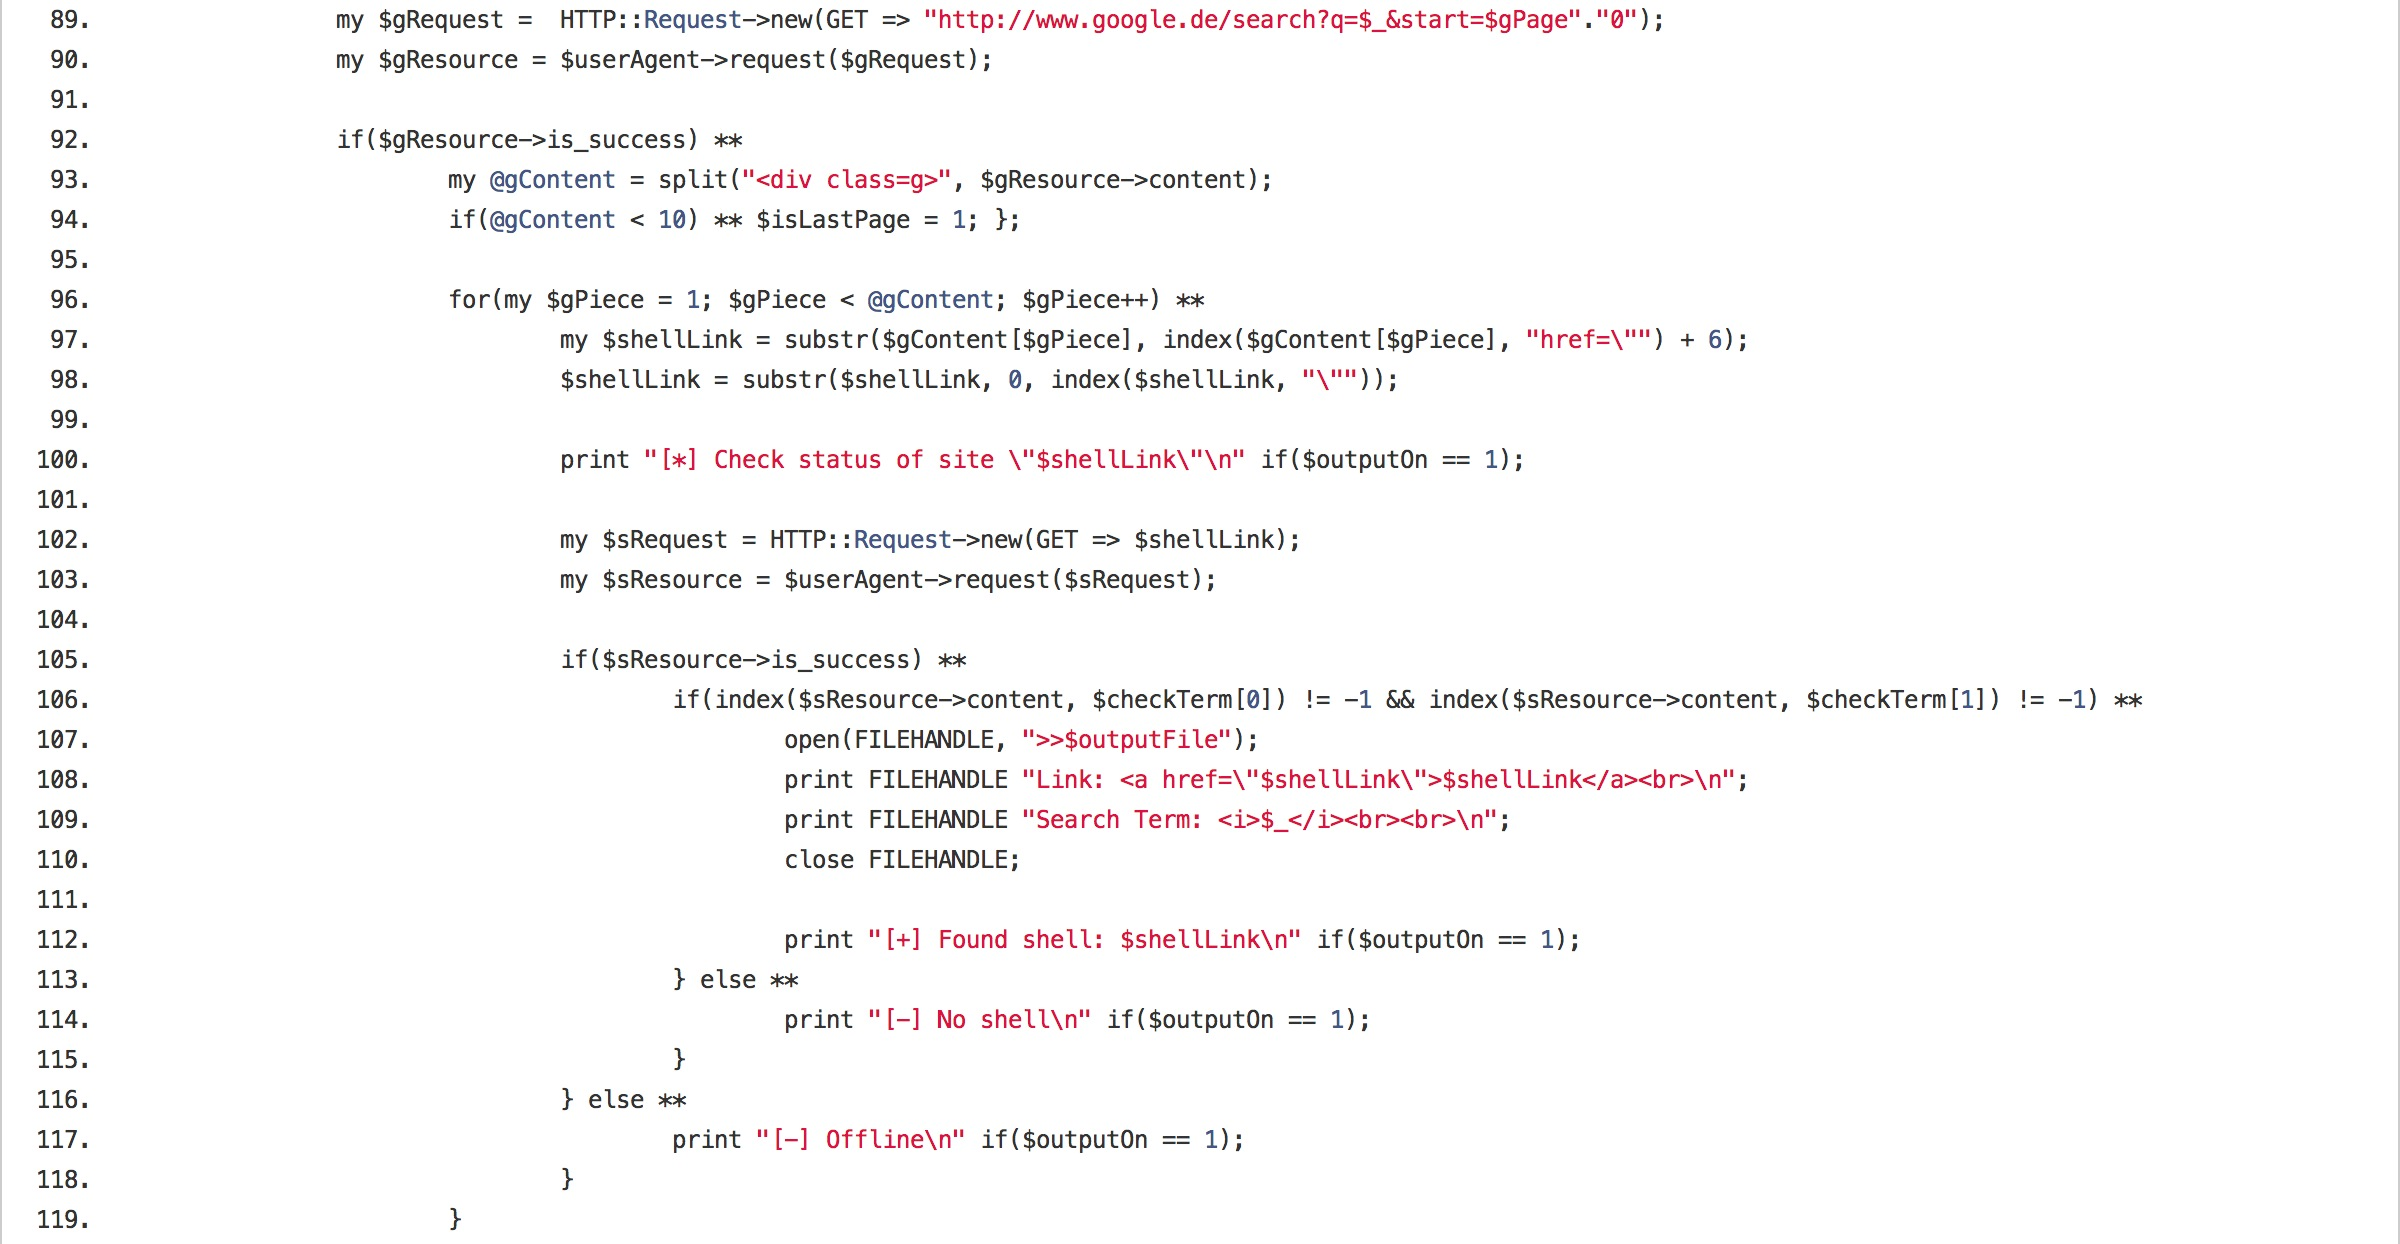
\includegraphics[width=0.8\textwidth]{Images/webSearchBot.jpg}}
\caption{Web search bot connecting to google.de\label{fig:webSearchBot}}
\end{figure}

\subsection{Network Scanner}

\begin{quote}
Number of Unique Files: 420\\
Number of Total Files: 445\\
Ratio (Unique/Total): 94.4\%
\end{quote}

Network scanning is one of the oldest reconnaissance methods. The attacker basically tries to look inside the internal network of the victim for any open port that can be used for performing an attack to a known vulnerable service. Several tools are available in the market, like Nessus \cite{nessus} and nMap \cite{nmap}. However, we didn't find any example of such softwares (even if we received commands aimed to launch an nmap session, even if the software is not present on our machines), while we received several examples of custom scripts aimed to discover internal hosts with known open ports, like FTP or TelNet. When an host with a known open port is discovered, a dictionary-based bruteforce attack is usually performed.

The example in Figure~\ref{fig:networkScanner} is the classical implementation of a network scanner: giving an IP address, the script creates a socket and tries to connect to that host on a certain port. If the connection is established, the result is displayed to the attacker. Among the ports scanned, we can recognize several known ports, as FTP (21), Telnet (23), SMTP (25) and NetBios (137, 138, 139).

\begin{figure}[H]
\centerline{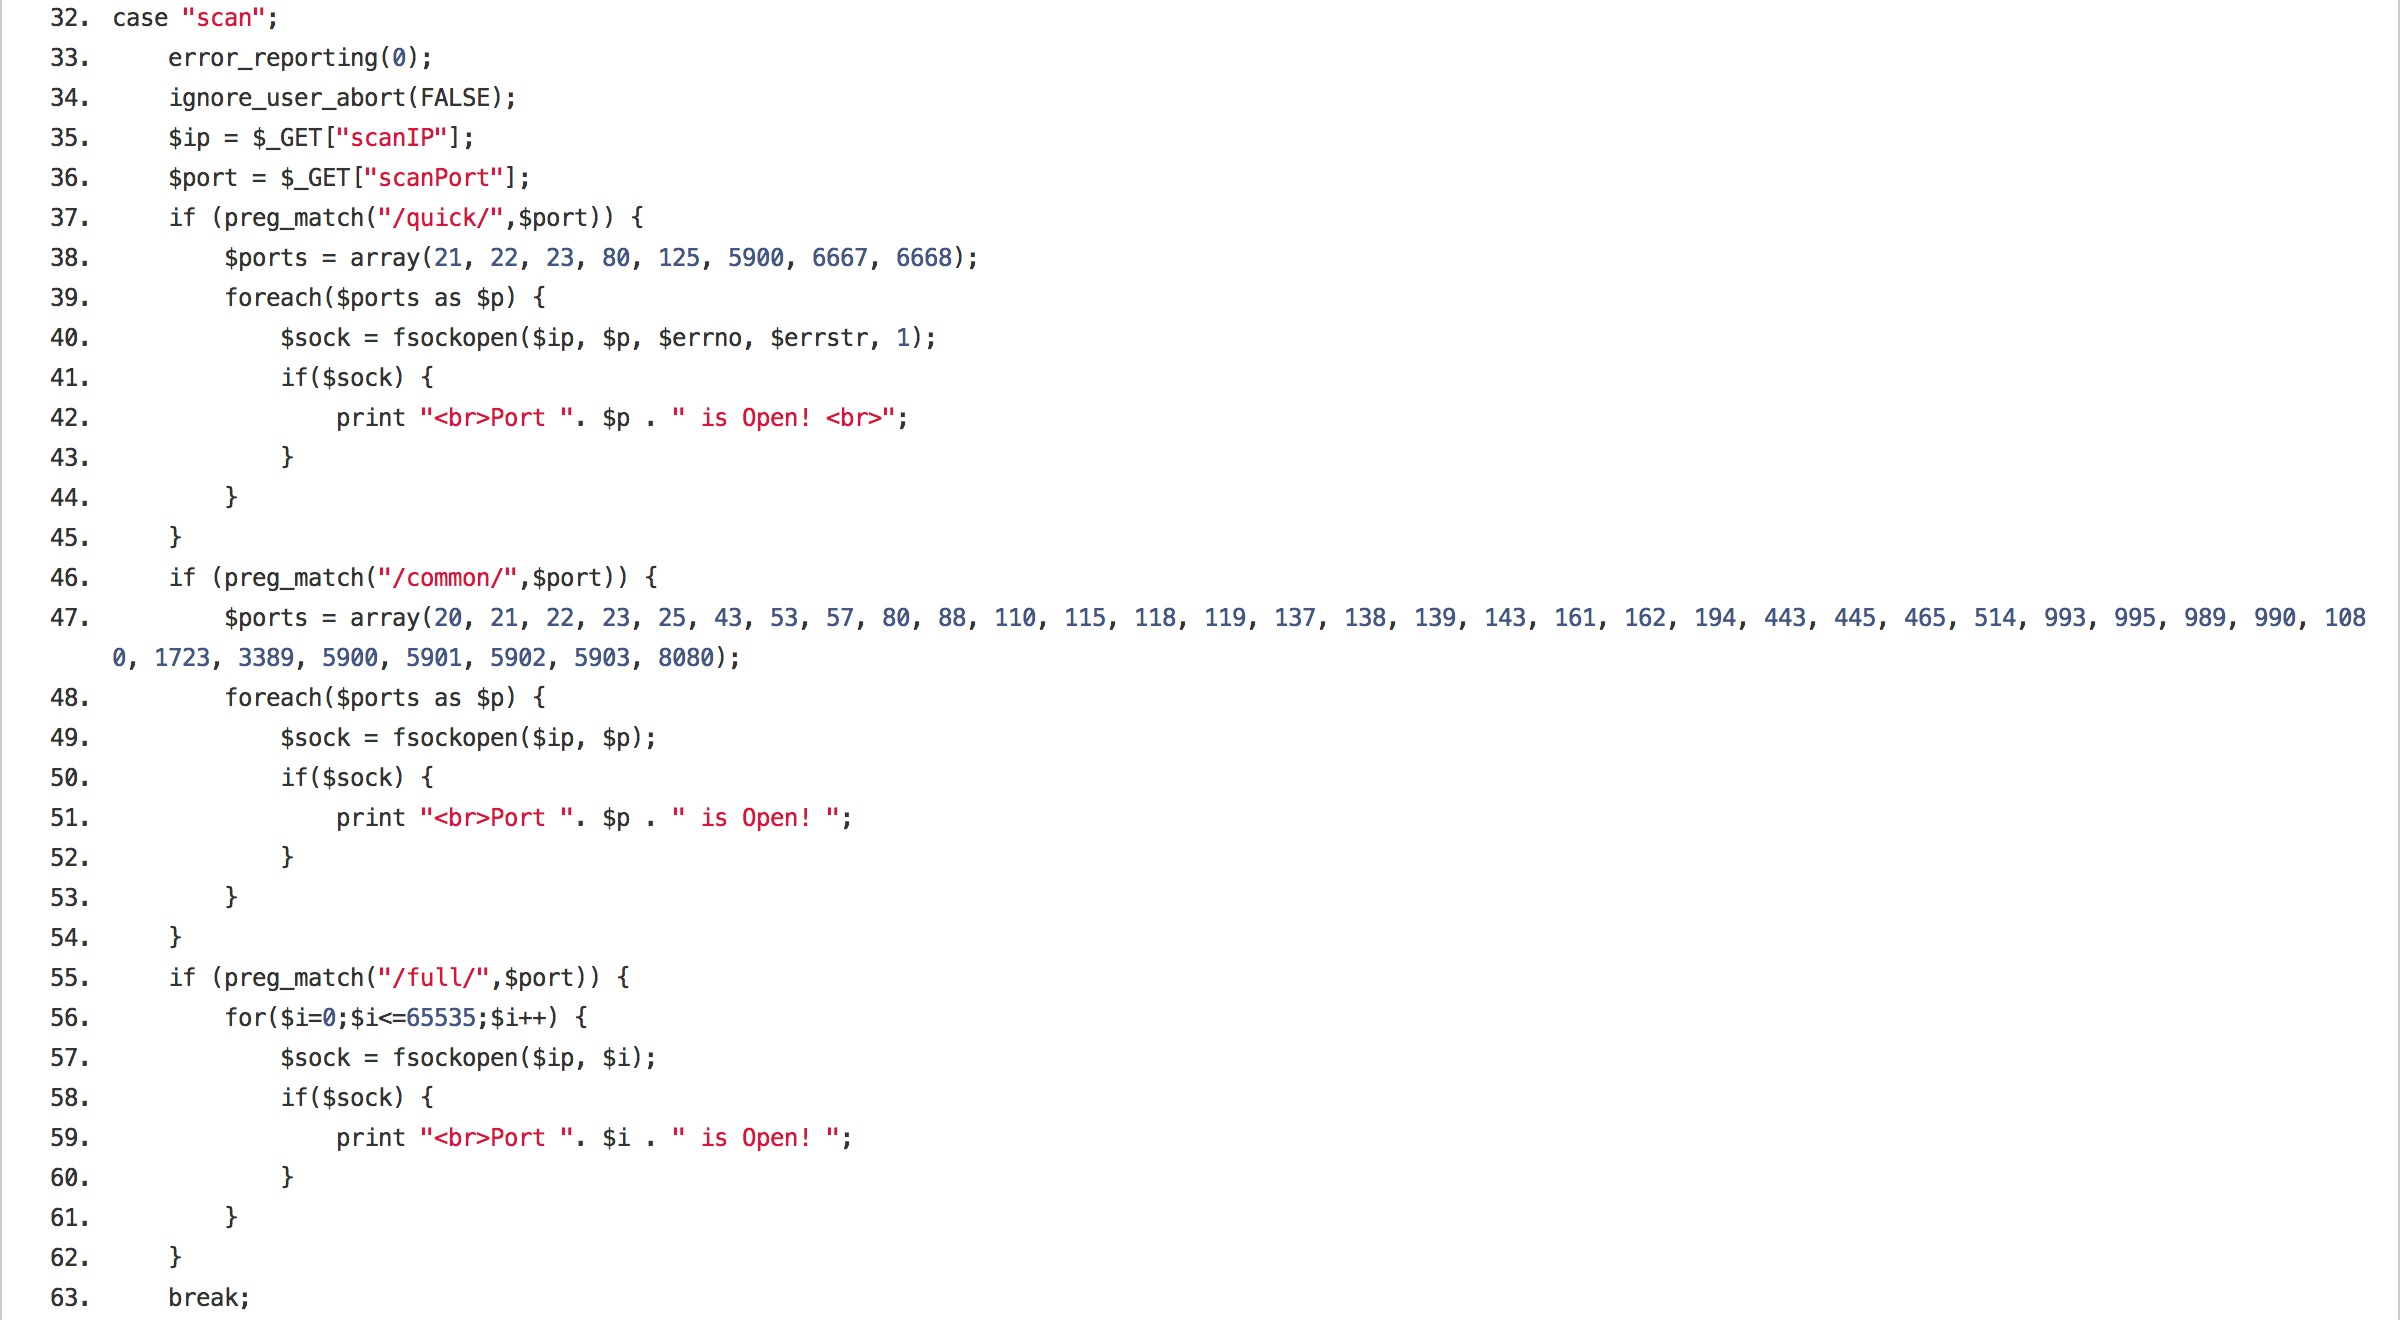
\includegraphics[width=0.8\textwidth]{Images/networkScanner.jpg}}
\caption{Network Scanner for well known ports\label{fig:networkScanner}}
\end{figure}

\subsection{Malware}

\begin{quote}
Number of Unique Files: 475\\
Number of Total Files: 492\\
Ratio (Unique/Total): 96.5\%
\end{quote}

Malware is one of the most common categories of malicious software present in the wild. It can be generally described as a tool intended for disrupt computer operations, gather sensitive information, or gain access to private computer systems. While there are several types programs that can be categorized as malware (viruses, trojan horses, ransomwares, spywares etc.) we preferred to group all these categories in one. We initially didn't expect to receive any example of this category, as malwares are usually targeting clients rather than servers, and the vast majority of them (over 99\% according to German anti-virus Firm G-Data \cite{malwWin}) are meant to be run on Windows environment, while most of the server are running some Unix distribution (Debian in our specific case). However, we received some example of malwares, most of them prepared to run on Windows 32 bits. The explanation to this behaviour is that our exploited machine has been used, according to the attacker's intention, as a ``storage facility'' for malwares. Furthermore, we analysed HTTP requests for these files, especially the Referrer Header, and we concluded that most of the times requests were coming from legitimate websites (mail clients, forums, etc.). We can conclude that the attacker tried to host the malware on our machines, while performing some kind of spamming campaign on other websites for spreading the malware and reaching more victims.

We analysed all executable files by sending them to VirusTotal, a web application which runs different anti-virus software on an uploaded file in order to understand if it's a malware, and its classification (when provided). An API is available for universities and research centres, allowing us to automatize the process of sending files.

As can be seen in the example (Figure~\ref{fig:malware}) VirusTotal correctly identifies the file as a Trojan Dropper \emph{Win32.Bladabindi}. In particular, this Trojan opens a backdoor for receiving communications from the attacker on port 8334, modifies the ``CurrentVersionRun'' Registry Key in order to be executed on Windows boot and logs every key pressed by the victim, sending daily reports to ``shaaa1983.zapto.org'' server.


\begin{figure}[H]
\centerline{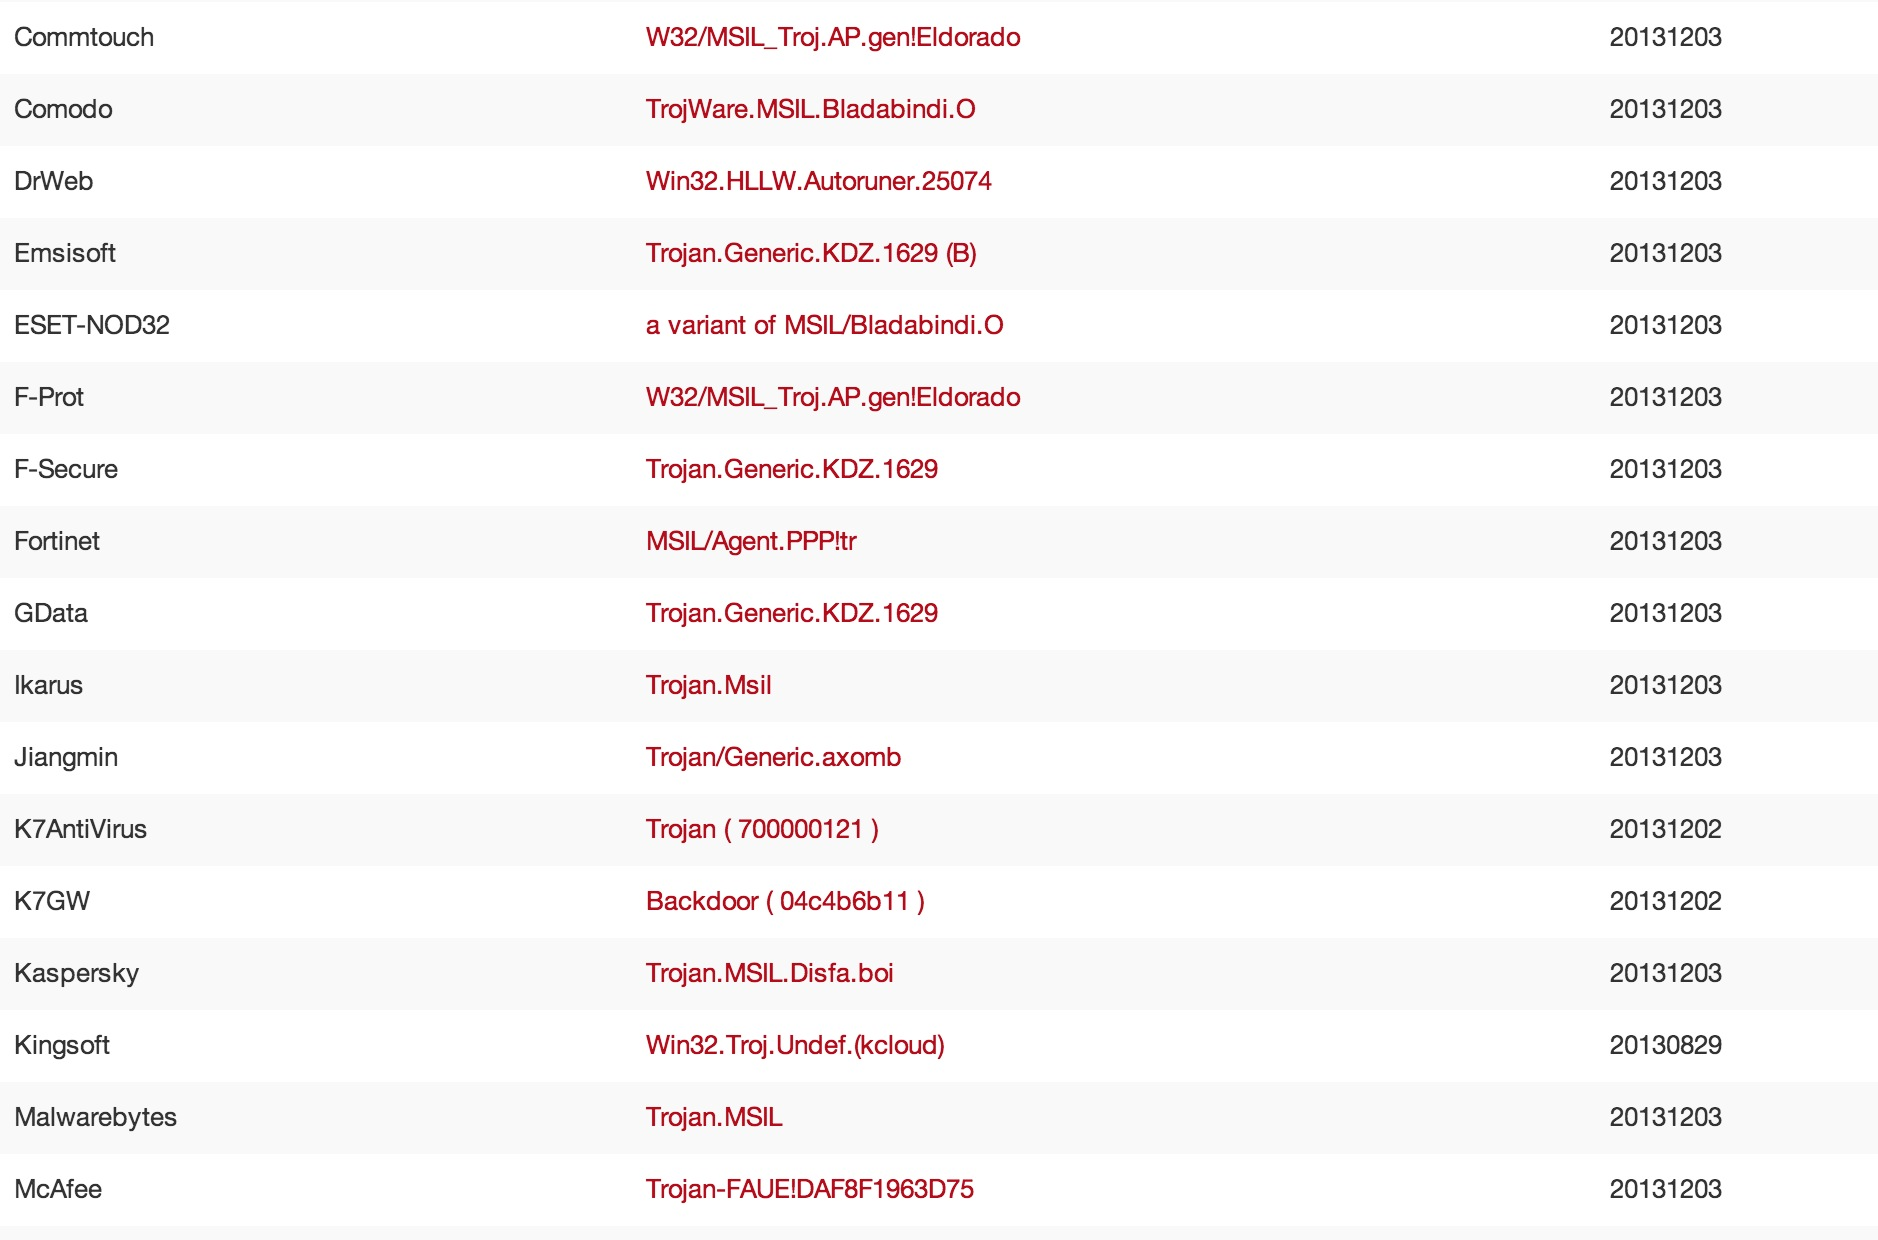
\includegraphics[width=0.8\textwidth]{Images/malwareVT.jpg}}
\caption{VirusTotal Report for Win32.Bladabindi\label{fig:malware}}
\end{figure}

\subsection{Documents}

\begin{quote}
Number of Unique Files: 516\\
Number of Total Files: 518\\
Ratio (Unique/Total): 99.6\%
\end{quote}

We included in this category every sort of files that can not be directly used as a tool or without any specific purpose. We carefully remove any private information as soon as we collect them (e.g., credit card numbers, mail addresses, phone numbers etc.) by means of regular expressions. We believe attackers use exploited servers for transferring contents. Most of them are related to spamming/phishing campaign, as list of mail addresses, but we also received several unrelated documents, from religious manifests up to manuals for creating bombs. In order to separate malicious documents, like malicious PDFs from other documents, we tested the document on VirusTotal application. We consider it as ``Document'' only if no anti-virus are considering it as a harmful file.

For example, we can see in Figure~\ref{fig:documentExample} an extract from one of these documents: in particular this text file is a cheat sheet for GTA San Andreas. The cheats are actually working.

\begin{figure}[H]
\centerline{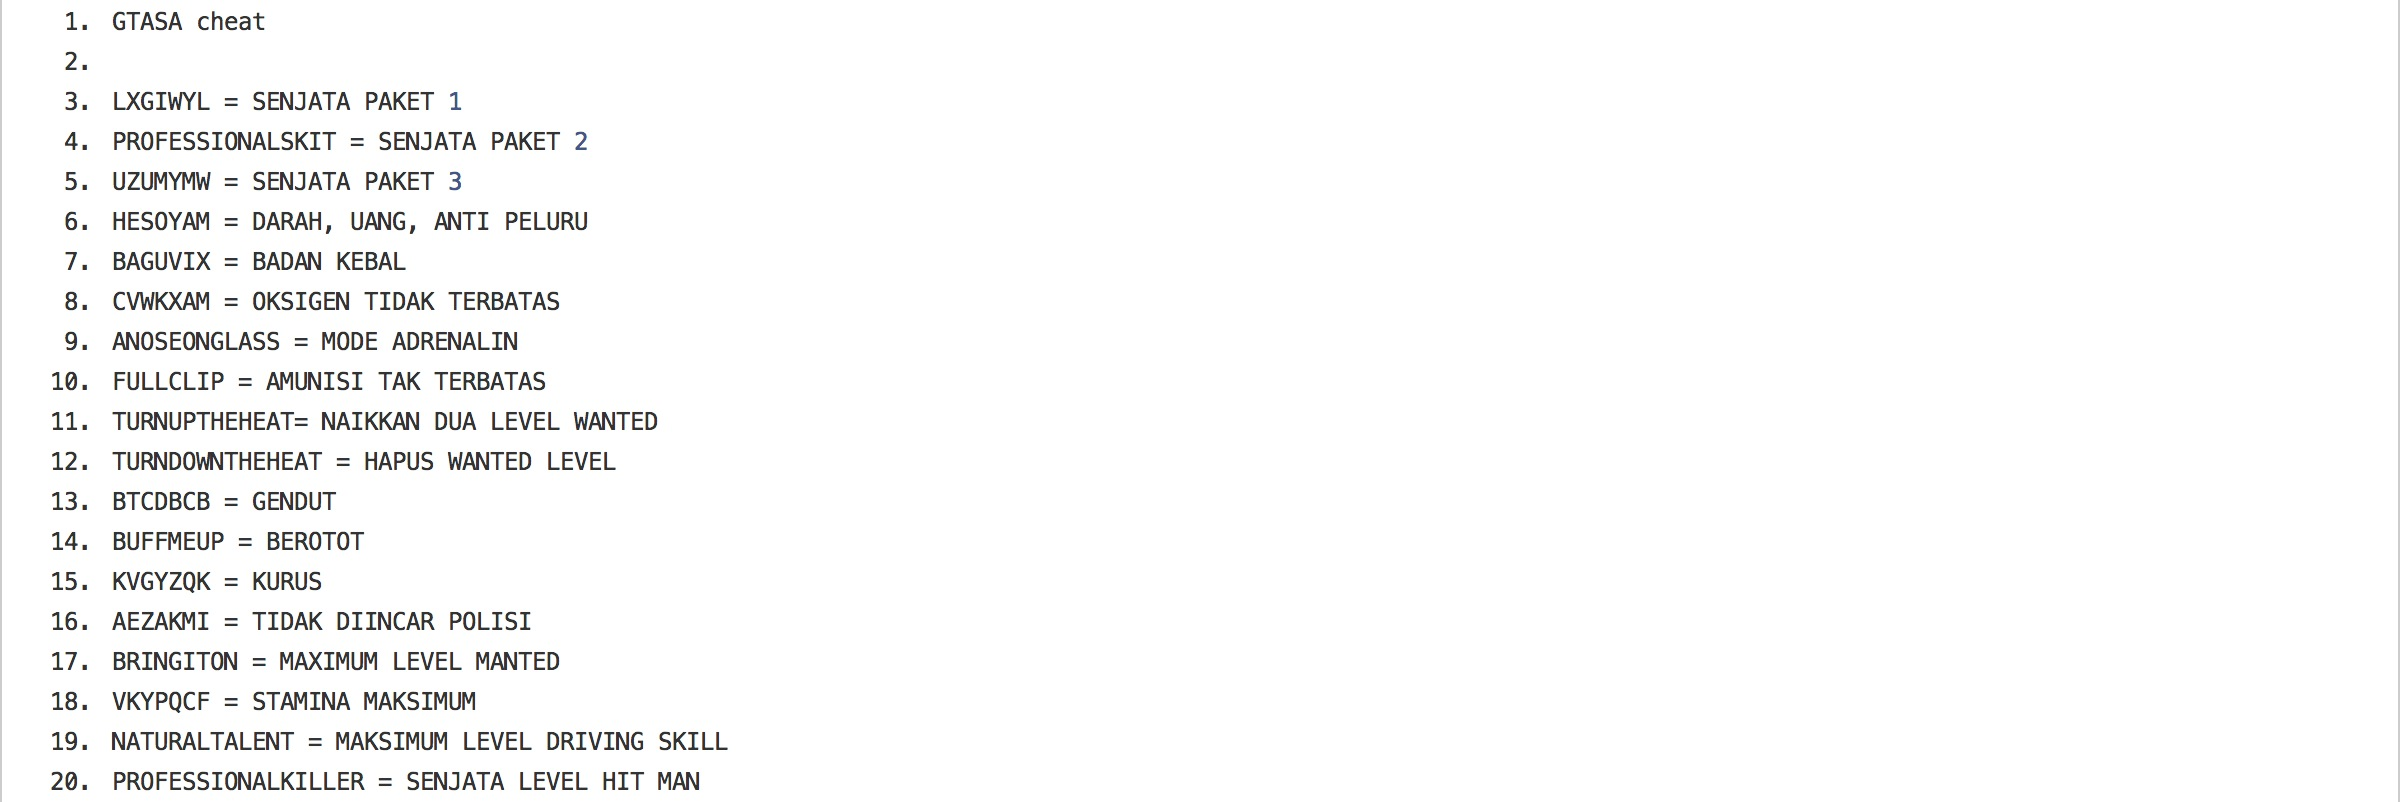
\includegraphics[width=0.8\textwidth]{Images/documentExample.jpg}}
\caption{Extract from GTA San Andreas Cheat Sheet\label{fig:documentExample}}
\end{figure}

\subsection{Uploader}

\begin{quote}
Number of Unique Files: 597\\
Number of Total Files: 740\\
Ratio (Unique/Total): 80.7\%
\end{quote}

One of the first objective an attacker tries to accomplish during the exploitation is to upload his own files on the machine. An uploader is a script exactly performing this operation: it allows the attacker to upload files on the web server. We generally recognized two types of uploaders, the ones receiving a file via a POST request and the ones which are aimed to receive a link to a file hosted on another web machine. Both of them are very interesting for us, as files directly uploaded on our honeypots can be clustered on our clustering system, while requests allow us not only to download and cluster the file, but also to log the request for future analysis.

In Figure~\ref{fig:uploader} we can see a classical example of an uploader: The PHP script is displaying a form where the attacker can copy and paste the content of a file and a path, on submission the file will be saved in the desired location.

\begin{figure}[H]
\centerline{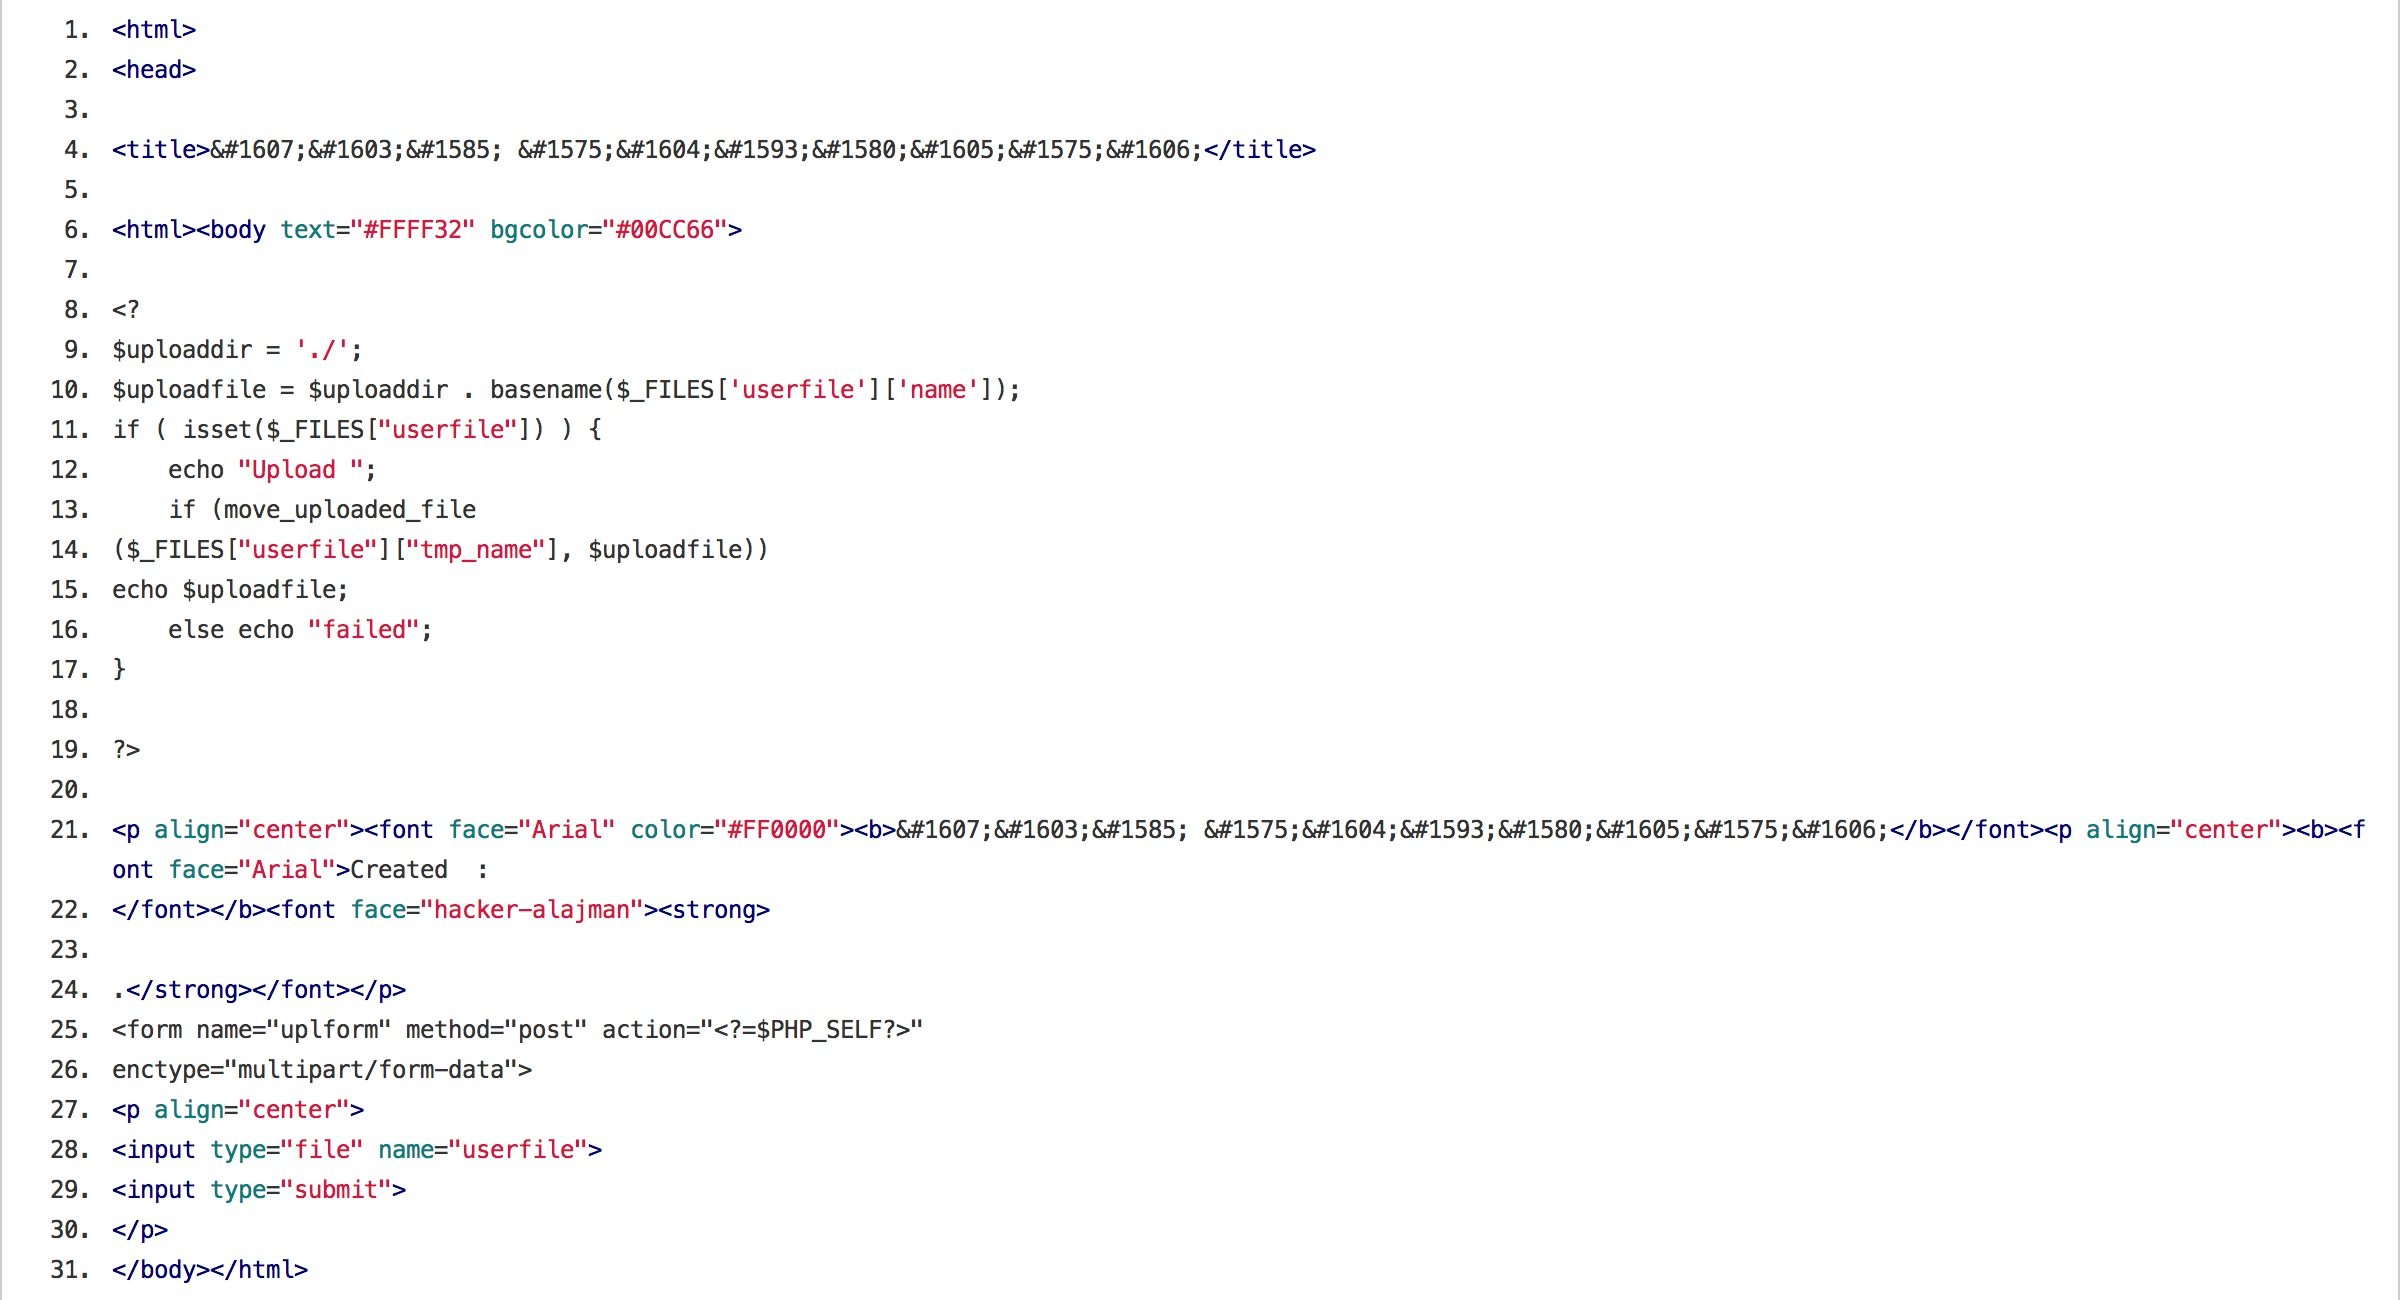
\includegraphics[width=0.8\textwidth]{Images/uploader.jpg}}
\caption{Example of Uploader script\label{fig:uploader}}
\end{figure}

\subsection{Configuration Overloader}

\begin{quote}
Number of Unique Files: 656\\
Number of Total Files: 713\\
Ratio (Unique/Total): 92.0\%
\end{quote}

We define as a Configuration Overloader any script aimed to rewrite several configuration files, like php.ini, .htaccess and similar. We also include in this category files that perform only the first operation described in a Mass Defacer, creation of symbolic links for substituting pre-existent pages to a new one. The main difference between a Mass Defacer and a Configuration Overloader is the missing ``defacement phase'' in the latter one.

As can be seen in Figure~\ref{fig:configOverload}, the typical Configuration Overloader writes a custom ``.htaccess'' file with several common options, like rewriting the Directory Index in order to redirect the index.html page on a page for a specific folder, and the option for following symbolic links, as the next step performed will be to overwrite all pages (in this specific example, pages from OSCommerce CMS) with a link to a custom page.

\begin{figure}[H]
\centerline{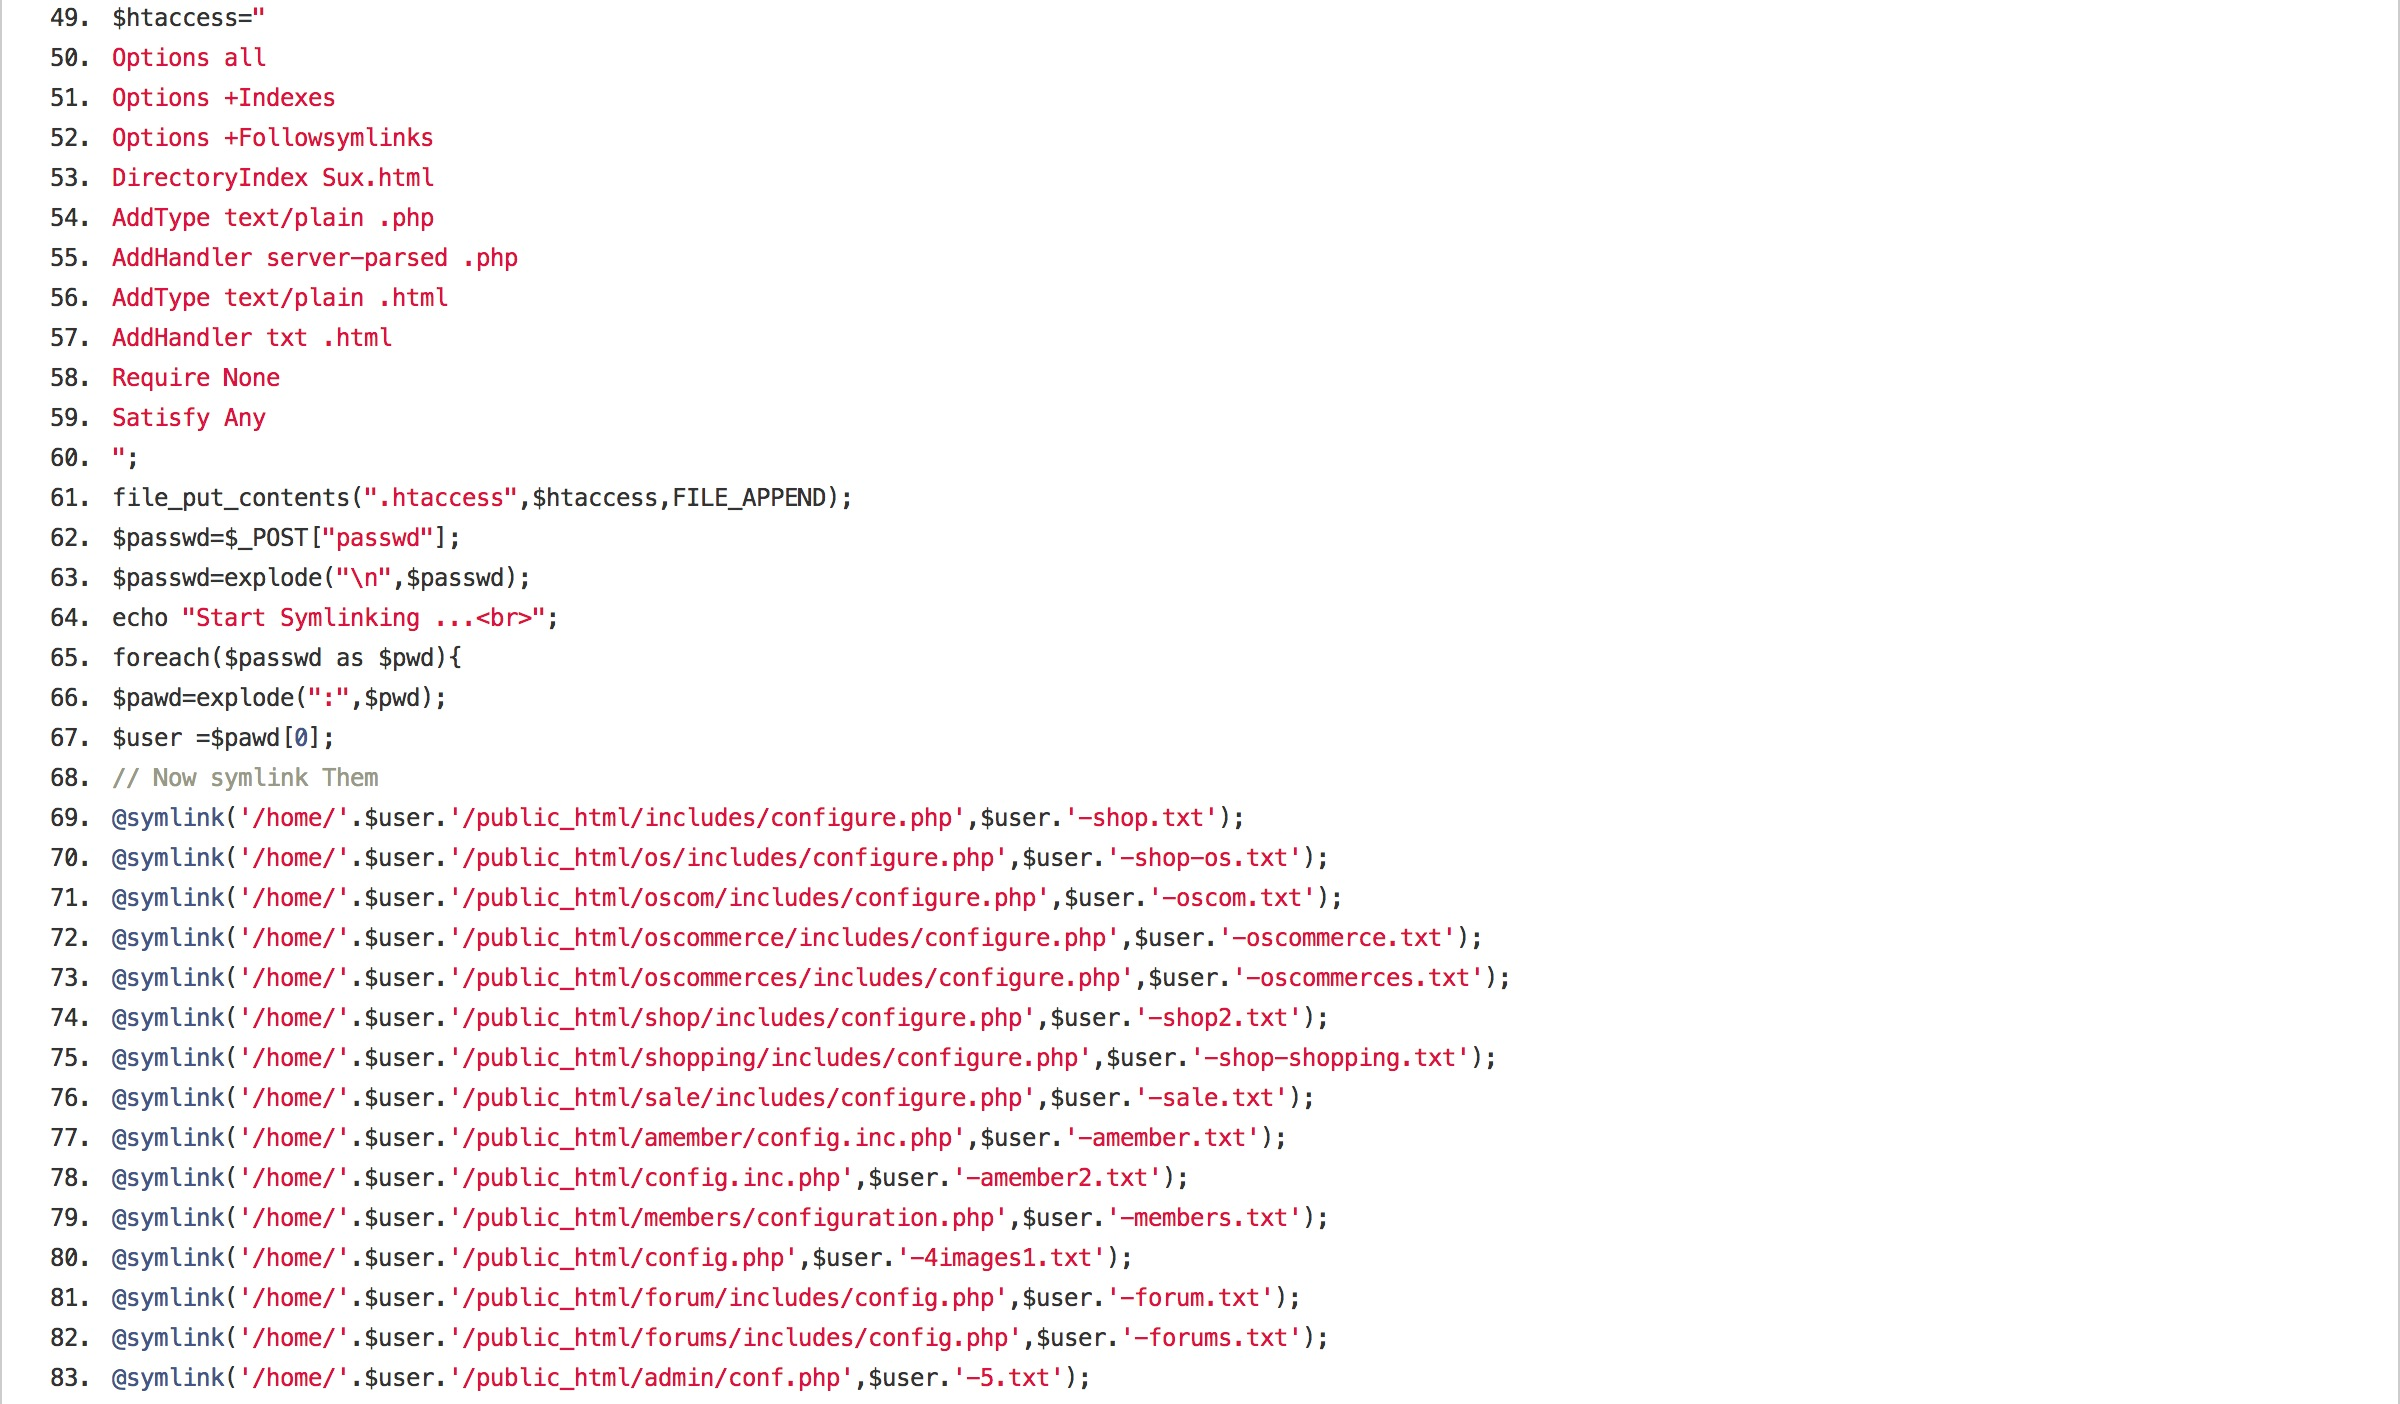
\includegraphics[width=0.8\textwidth]{Images/configOverload.jpg}}
\caption{htaccess rewrite and symlinks creation on a Configuration Overloader\label{fig:configOverload}}
\end{figure}

\subsection{BackDoor}

\begin{quote}
Number of Unique Files: 703\\
Number of Total Files: 728\\
Ratio (Unique/Total): 96.6\%
\end{quote}

Inserting a backdoor is a common technique for attackers in order to maintain access to an exploited web server even after the webbmaster rebooted the machine. This kind of tools, in fact, are usually uploaded to a hidden directory (attackers usually tried to put these files in /usr/bin or /lib/ directory, with a name starting with ``.'' character in order to become invisible with regards to \emph{ls} command). In order to let these programs work even after a reboot, criminals usually try to add an entry on a rc script (like /etc/rc.2, /etc/rc.local), or add it in the crontab. Inside this category we find several different type of files, from ELF executable to Perl, PHP and Python scripts.

This kind of files is usually opening a socket on a custom port and listening to that port for any connection. Usually, when a connection is received a password is asked and, if positive, a shell is executed in order to allow the connector to launch arbitrary shell commands on the web server. Another version of these scripts are actively connecting to a remote host (usually hardcoded or given as a argument parameter) and keeping the connection active. The attacker has only to give commands to a single machine which in turn will send this command to all shells connected to it, like a C\&C server in a botnet.

We show in Figure~\ref{fig:backDoor} the main loop of one of these backdoors: working as a server, the script is using an infinite loop (while true) waiting for any connection and spawning a shell to each client. Not shown in the image is the content of the ``Shell'' class, where a password (hardcoded inside the script) is asked to the client. If this check fails, the connection will be dropped.

\begin{figure}[H]
\centerline{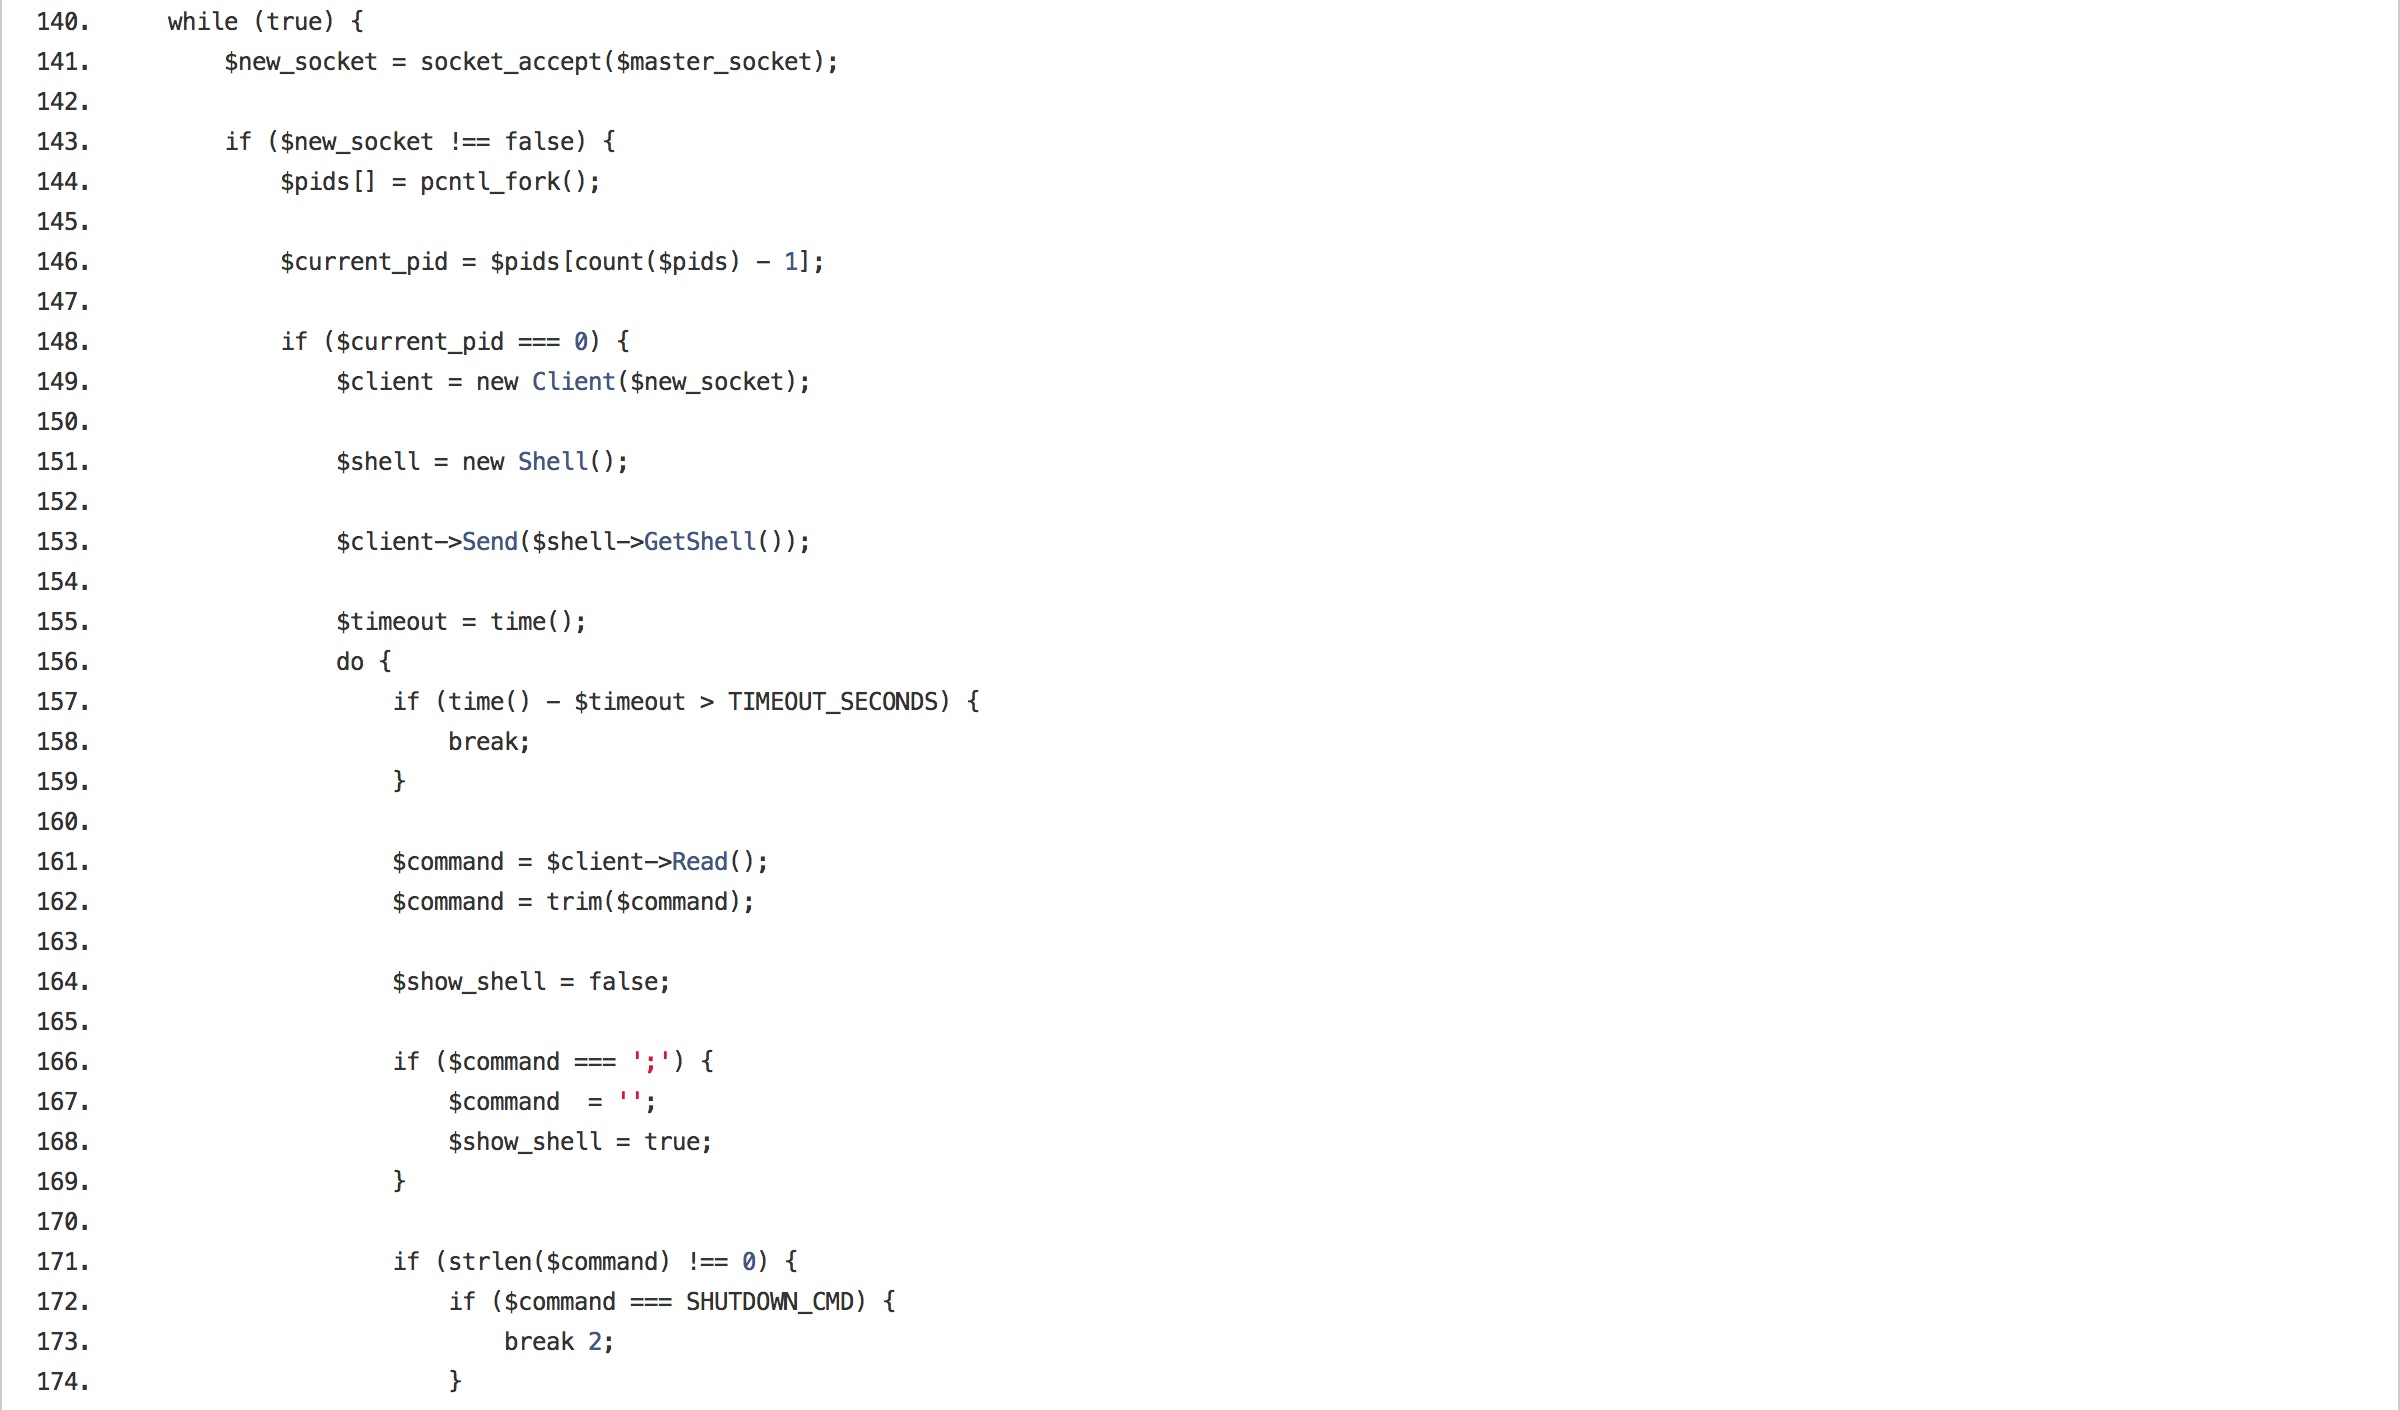
\includegraphics[width=0.8\textwidth]{Images/backDoor.jpg}}
\caption{Main loop of a Backdoor\label{fig:backDoor}}
\end{figure}

\subsection{BruteForcer Script}

\begin{quote}
Number of Unique Files: 1757\\
Number of Total Files: 1959\\
Ratio (Unique/Total): 89.7\%
\end{quote}

A BruteForcer Script is a tool aimed to attack a specific service by means of brute-forcing attack. We actually bend the strict definition of bruteforcing as we do not only include in this category cryptanalytic attacks which systematically check all possible passwords by traversing the entire search space, but also any kind of dictionary-based attack, where passwords checked belong to a dictionary. The dictionary can be directly hardcoded inside the script, increasing by many order of magnitude the size of the file, or being loaded from another file during the attack. A third possibility is represented by dynamically receiving a list of password via a POST request. The target of these scripts can vary: we received files meant to guess user and password of a local database, or meant for bruteforcing FTP protocol of a remote host, and several other examples.

Another example of bruteforcing script is directed to particular web applications. During our experiments, we received scripts directed toward Apple web server and Sky web server: in particular, these two web services allowed for username and password checking without tracking the number of requests performed from a single IP address. This behaviour allows an attacker to discover valid username and password couples by simply performing endless requests. Some of these scripts are loading their dictionaries from uploaded files, and these files showed how tested words belong to specific alphabetic ranges. Our conclusions from this analysis is that attackers are parallelizing a dictionary-based bruteforce attack over these specific web servers by uploading the same script and different parts of the same dictionary to different exploited web servers.

The script shown in Figure~\ref{fig:bruteForcer} is loading a list of usernames and passwords directly from a POST request, and then trying each couple with two possible targets, according to a parameter passed to the script. ftp\_check is checking the couple on the FTP service of an external web server, while cpanel\_check is checking the cPanel web interface (port 2082). cPanel is a Unix based web hosting control panel that provides a graphical interface and automation tools designed to simplify the process of hosting a website, utilizing a 3 tier structure that provides capabilities for administrators, resellers, and end-user website owners to control the various aspects of website and server administration through a standard web browser. It's easy to understand why attackers can be interested in discovering credentials for accessing this service, as it'd give them possibility to fully control the web server.

\begin{figure}[H]
\centerline{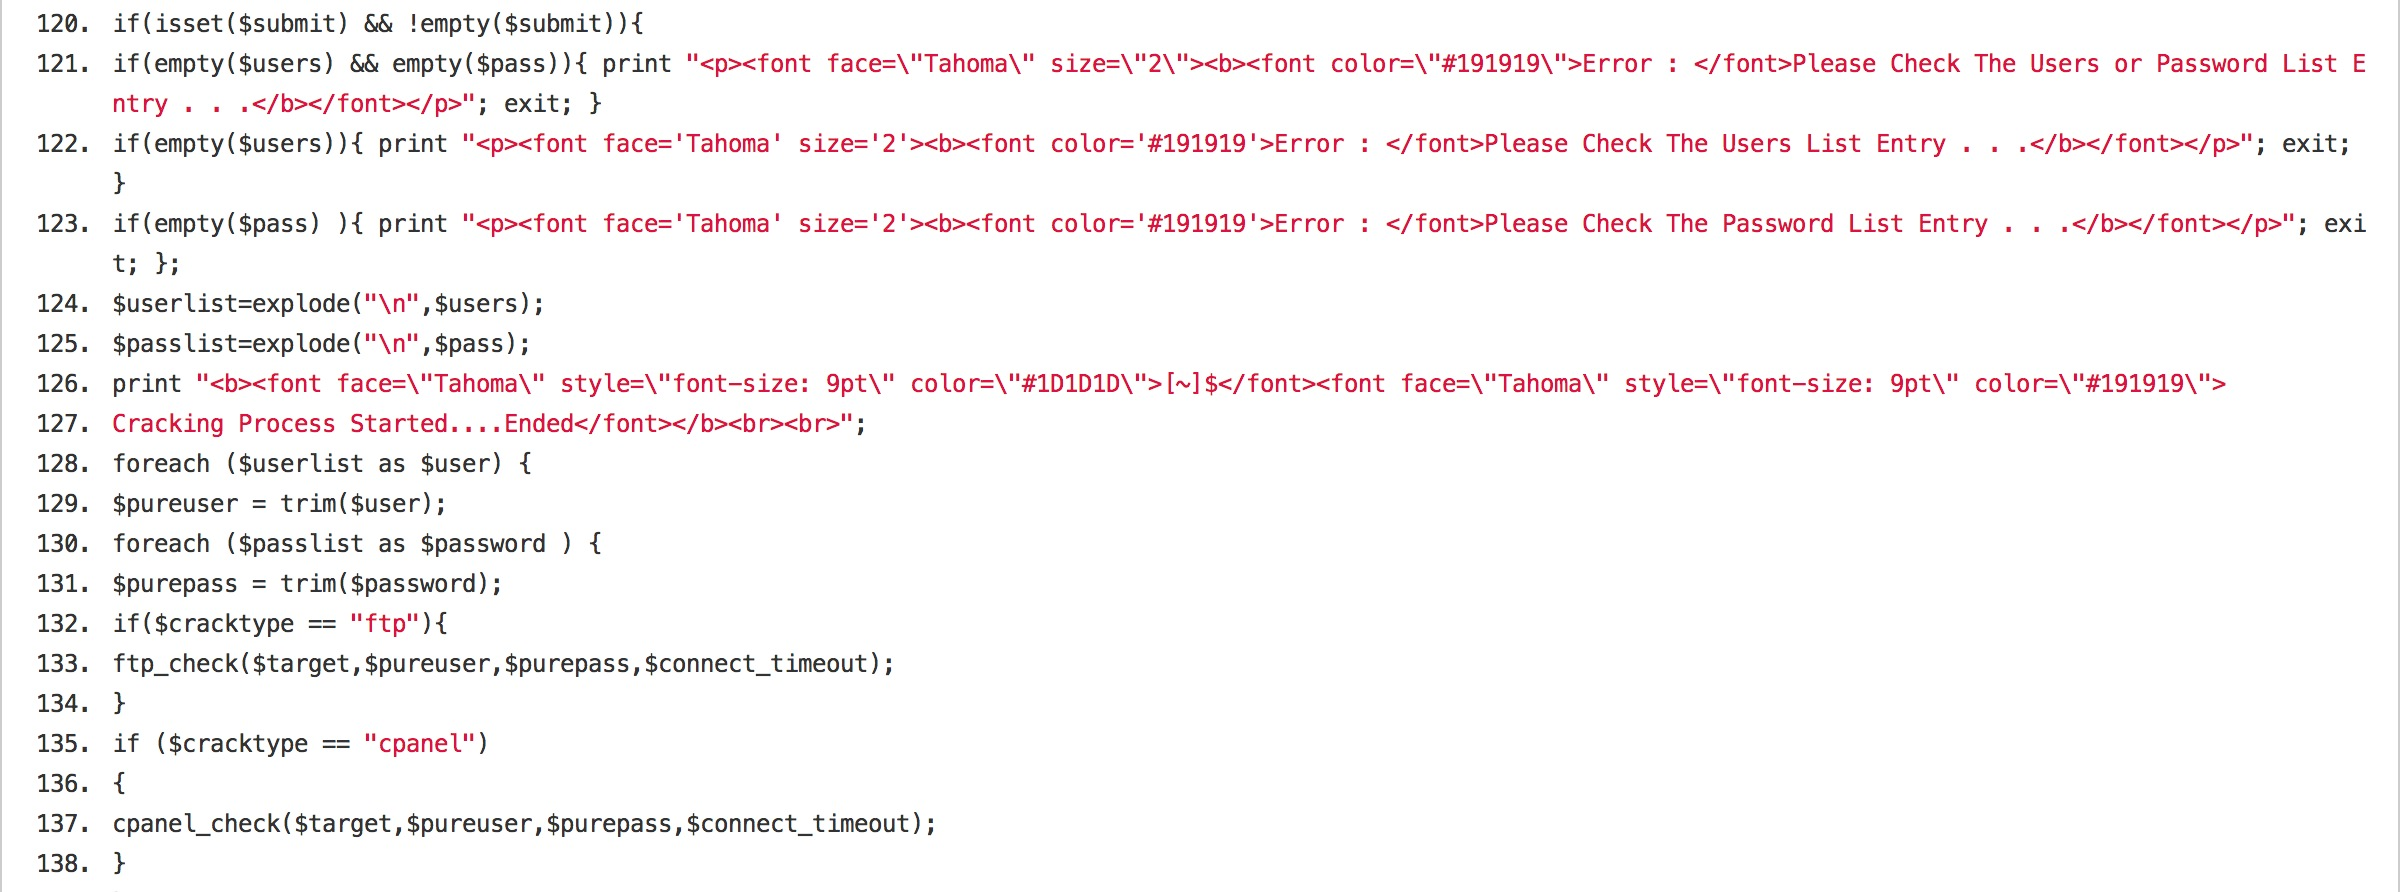
\includegraphics[width=0.8\textwidth]{Images/bruteForcer.jpg}}
\caption{Main loop of a Backdoor\label{fig:bruteForcer}}
\end{figure}

\subsection{Local Exploit}

\begin{quote}
Number of Unique Files: 2033\\
Number of Total Files: 2322\\
Ratio (Unique/Total): 87.5\%
\end{quote}

We consider as a local exploit every tool that aims to increase the privileges of the web user on the machine. In this category we included two different kind of programs: single executables (or at least source files), and scripts aimed to download and execute automatically a local exploit. Both of them eventually rely on a known vulnerability on our system (both inside the kernel or inside a setuid executable) in order to exploit it and acquire root privileges on the machine.
This category of attacks is actually impossible to be avoided: we can't be protected against any 0-day vulnerability on Linux Kernel or on one of the services hosted on our machines. However, we mitigated this problem by automatically update every single part of the basic snapshot (the virtual machine image that will be used for restoring the web server after every completed attack) and by limiting the number of services available on the machine.

It's important to notice how these files, even if the ratio Unique/Total is quite high (>85\%), are rarely directly written by the attacker: building an exploit is not an easy task and it's usually performed by some highly skilled professionals, who are releasing the exploit in the wild. Attackers simply grab the source code, compile it (usually directly on the exploited machine) and run it against the web server. The only exception to this behaviour is represented by scripts which are downloading and executing exploits, as the source from which exploits are downloaded can vary. In particular, source code can be downloaded from some public exploit databases (like exploit-db.com or 1337days.com), from some private servers (usually under control of the attacker) or from some public code-hosting web service (like code.google.com or github.com).

An example of the last category of scripts is displayed in Figure~\ref{fig:localExploit}. In this particular case, the script (written in Perl) is downloading several different source code files from \emph{www.r00tw0rm.com} website, a commonly known exploit database which have been recently shut down by US government, compile (after eventually unpacking the archive) them using gcc (we installed autotools on our honeypots in order to allow this behaviour), launch the exploits and checking the id of the user after each exploit run. If any of the attacks has been successful, the id displayed would be 0, which is the root id on Unix systems.

\begin{figure}[H]
\centerline{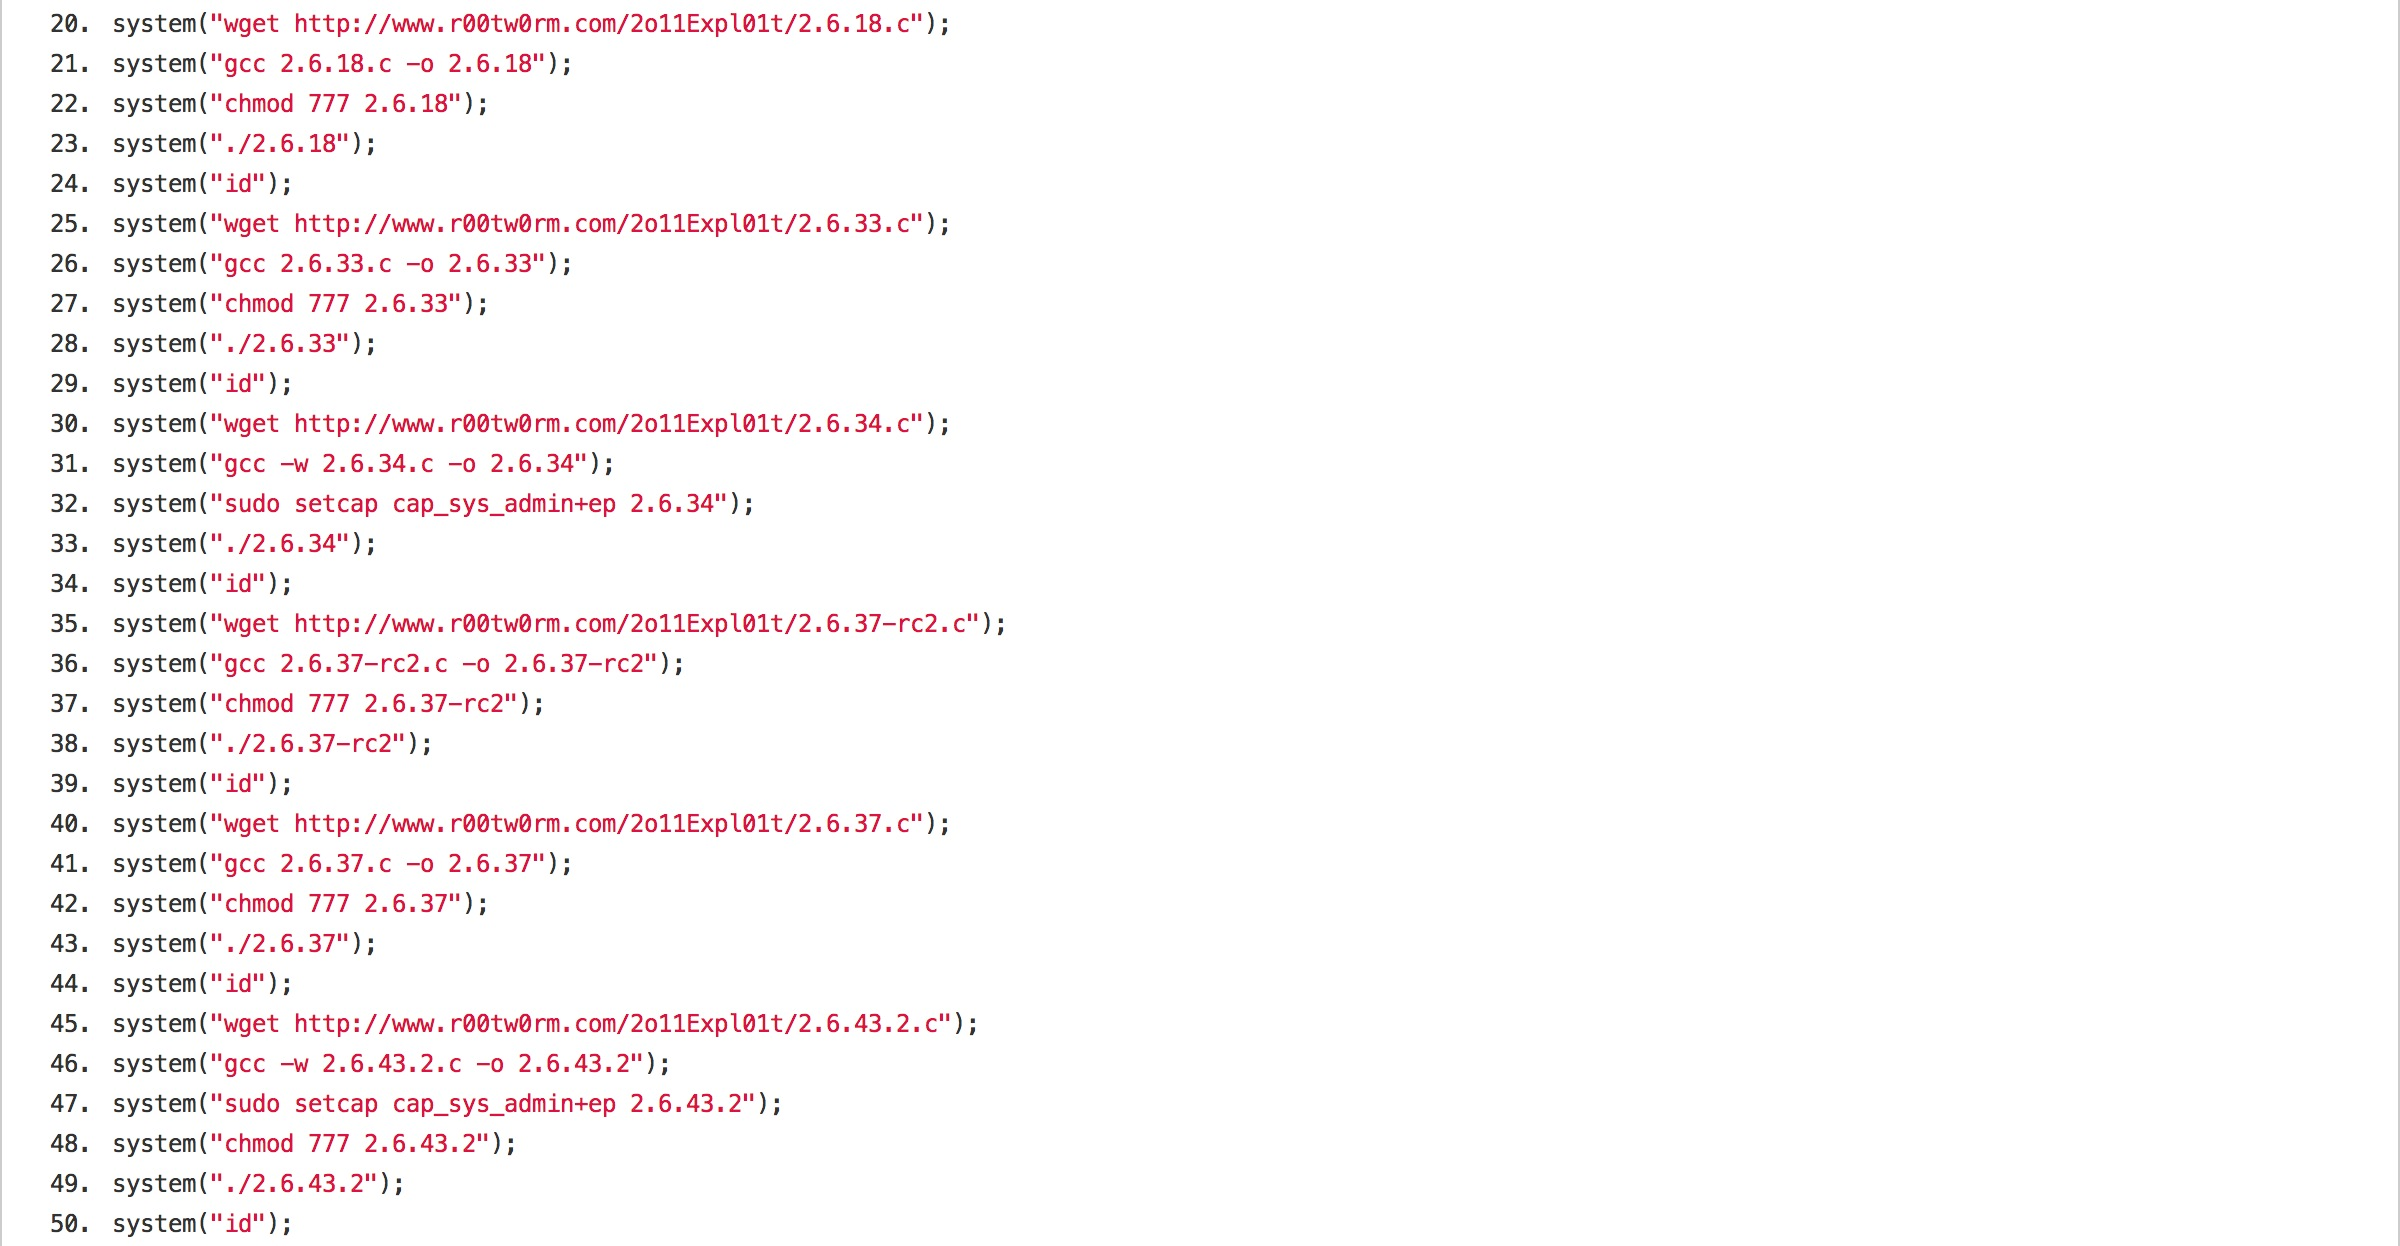
\includegraphics[width=0.8\textwidth]{Images/localExploit.jpg}}
\caption{Download, compile and launch of several exploits for Unix kernel\label{fig:localExploit}}
\end{figure}

\subsection{Flooder Script}

\begin{quote}
Number of Unique Files: 2841\\
Number of Total Files: 2952\\
Ratio (Unique/Total): 99.6\%
\end{quote}

A Flooder Script is any script that aims to compromize the usability of a server by means of flooding attack. This is a particular case of a DoS (Denial Of Service) attack relying on the transmission of several crafted packages to the same web server in order to cause the crash of a particular service (even the whole machine on some configurations).

There are several options for performing a flooding attack on different protocols, from UDP flooding (which is performed by sending the same packet on several random UDP ports)up to HTTP flooding (performed by sending specially crafted HTTP requests). In the latter case, as in TCP flooding, it must be noticed that the packet should be manually crafted and not relying on the usual protocol stack, otherwise the attacker should open and maintain an open connection for each TCP packet, provoking a DoS on his very own machine.

Figure~\ref{fig:flooder} shows a typical example of a UDP flooder. The code sends a dummy packet (composed of 65,000 ``X'' characters) to a random port of the victim. Each packet forces the victim into checking if there is a service listening on the port (in most case the answer will be no, as wanted by the attacker) and sending the appropriate response (for unused ports it will be an ICMP Destination Unreachable packet). This process would eventually cause the victim OS to crash. A nice optimization of this code would be to spoof the IP source address in order to avoid the ICMP response coming from the victim while it still active.

\begin{figure}[H]
\centerline{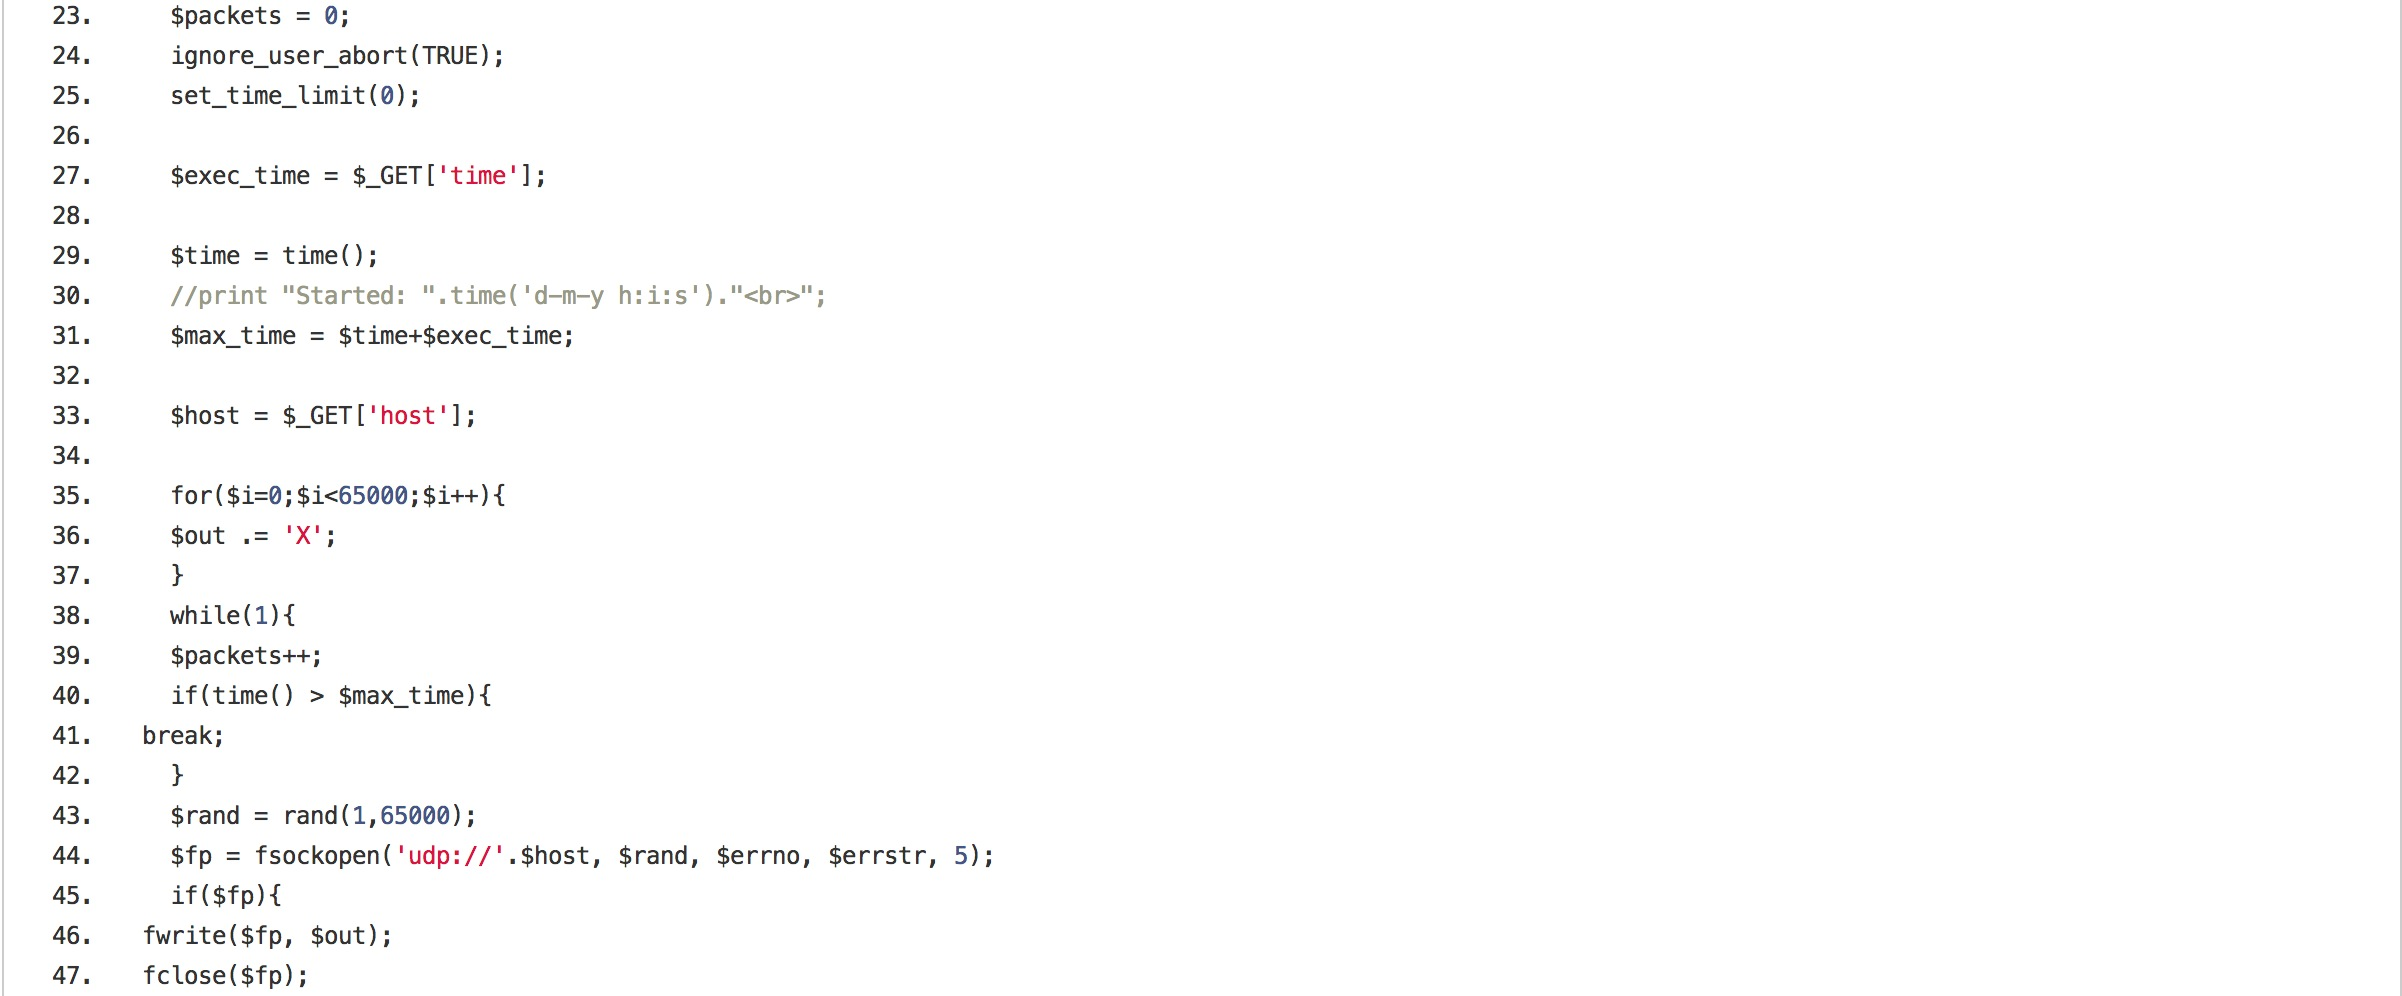
\includegraphics[width=0.8\textwidth]{Images/flooder.jpg}}
\caption{Main loop of a Backdoor\label{fig:flooder}}
\end{figure}

\subsection{Attack Scripts to other machines}

\begin{quote}
Number of Unique Files: 3956\\
Number of Total Files: 5064\\
Ratio (Unique/Total): 61.1\%
\end{quote}

We classified as ``Attack Scripts to other machines'' any script which is in charge of performing an exploitation toward an external machine. We defined exploit as any activity intended to leak private informations exploiting a victim machine not using any bruteforce attacks or flooding DoS. In this category we can find LFI/RFI Scanners, CMSs exploiter etc..

As in the Local Exploit category, this category of files is not usually written directly by an attacker. Instead, they are created by highly skilled programmers and reused by other attackers. Generally speaking, these kind of scripts receive a list of IPs/URLs and perform an attack over these candidates.
For scanners, these scripts are generally looking for LFI/RFI vulnerabilities: this kind of vulnerabilities (Local Files Inclusion/Remote File Inclusion) allows an attacker for displaying arbitrary files on the webpage of the victim. That is, an LFI would allow for an attacker to display /etc/passwd inside a webpage. An RFI works in the same way but by allowing an attacker to embed an arbitrary external page inside a webpage. The latter vulnerability is more dangerous as it allows an attacker to include a web shell on the victim, usually allowing it for arbitrary code execution in the victim environment.
A CMS exploiter, instead, looks for specific paths on a specific web application in order to exploit known vulnerabilities (like the ones we have on our honeypots), usually trying to upload a web shell on these machines and notifying the attacker of the successful exploitation.

In Figure~\ref{fig:attackerScript} we show an example of CMS exploiter. In particular, the script targets an arbitrary file upload vulnerability in img\_manager <=2.0.10 plugin for Joomla! \cite{joomlaImgManager}. The part shown, however, is meant for only checking the existence of the vulnerability (a patch issued by Joomla! developer make the request ending up in a 404) and not for actually exploit it. A successive part of the script (not shown) is in charge of the actual exploitation of the  vulnerability and the upload of a web shell on the target.

\begin{figure}[H]
\centerline{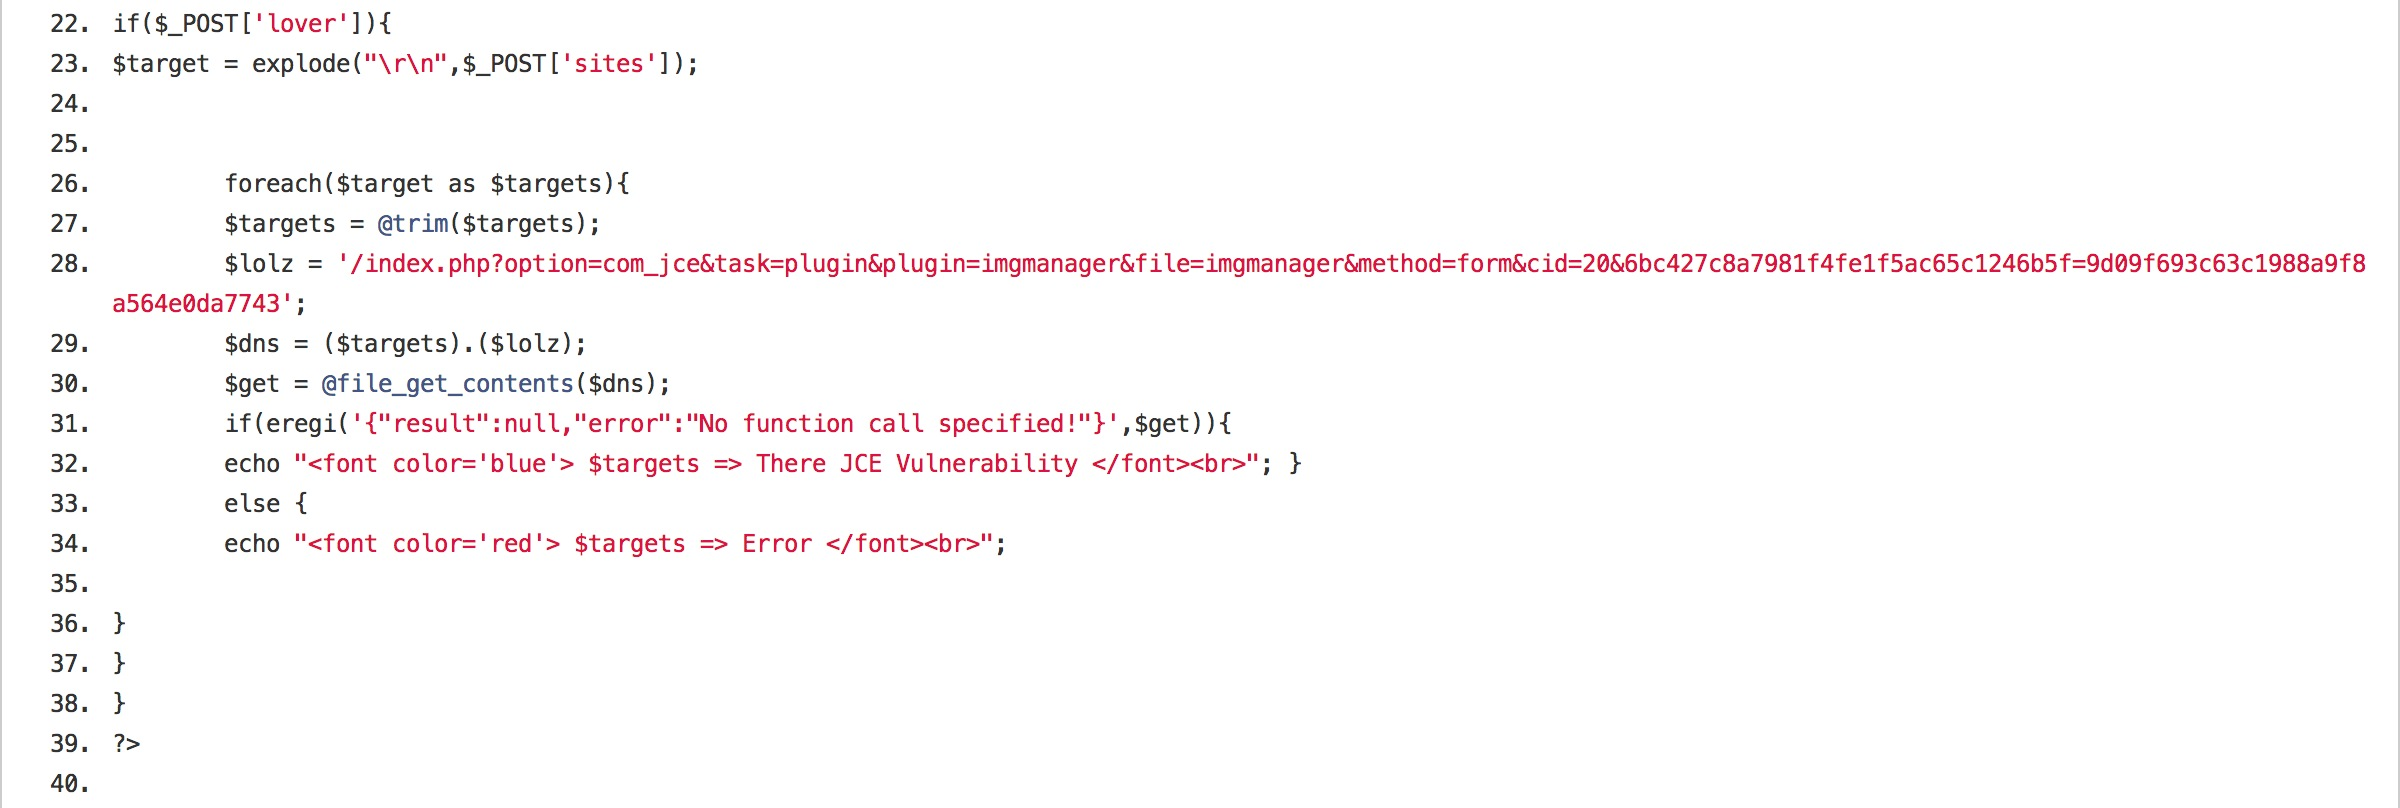
\includegraphics[width=0.8\textwidth]{Images/attackerScript.jpg}}
\caption{CMS Exploiter vulnerability detection phase\label{fig:attackerScript}}
\end{figure}


\subsection{Botnet}

\begin{quote}
Number of Unique Files: 6878\\
Number of Total Files: 7912\\
Ratio (Unique/Total): 86.9\%
\end{quote}

A Botnet can generically be described as a program communicating with other similar programs over the Internet in order to perform some tasks. This is one of the most common objectives pursued by attackers. By using a botnet, in fact, an attacker is able to parallelize attacks, perform Distributed Denial of Service attacks (DDoS), distributed bruteforcing and even bitcoin mining.

While we initially considered to receive a small number of these files, as they are usually meant to be run on clients rather than servers, we had to change our beliefs as it seems that the number of botnets which are including servers is constantly increasing over time. The reason behind this behaviour can be found in the fact that a server is a machine which is usually up and running 24 hours a day 7 days per week, while a client is usually turned off during the night. Therefore, attackers are looking up for uploading botnets also on servers in order to maximize the productivity of their networks.
Most of the botnets we received are in communication with other machines via IRC: this protocol (cfr. RFC 1459 \cite{irc}), invented in 1993 by J. Oikarinen and D. Reed, focuses on group communication in discussion forums by means of live interactive instant text messaging. Clients are connecting to one or more ``channels'', where they can see message posted by other clients. One or more of these clients work as administrators, having specific permissions over other clients (muting, kicking out etc.).
Another way of communication for botnets is over HTTP: clients periodically connect to a web server (usually by an URL, so that the IP can change over time), send to it a batch of informations and receive new instructions.
In a botnet, the administrator of the IRC channel or the web server clients are connecting to is called Command\&Control server. Using this one-to-many mechanism, attackers are able to maintain control and give new tasks to several machines by issuing commands to only one server. Furthermore, it allows for an easy way of updating scripts, as every single bot in a Botnet are connecting to the same C\&C. We drop any connection performed by our scripts, so that the C\&C will never acknowledge of the presence of a new bot inside the network. However, this behaviour prevents us to discover new updates issued by the botMaster to any script, and a particular study in this direction can be explored in future works.

The beginning part of a botnet script is shown in Figure~\ref{fig:botnet}. Starting from a set of hardcoded initial nicknames and IRC channels, on the first boot the script tries to connect to various channels until it receives the first answer. At this point it receives a first batch of updates and commands. Once the initial setup is completed, it will connect to different IRC channels using given nicknames and waiting for commands from C\&C. An initial group of commands are already present inside the script: this set include DoS attacks and bruteforce. However, the botMaster always have the possibility to issue new commands to every machine in the botnet by means of the generic execute function.

\begin{figure}[H]
\centerline{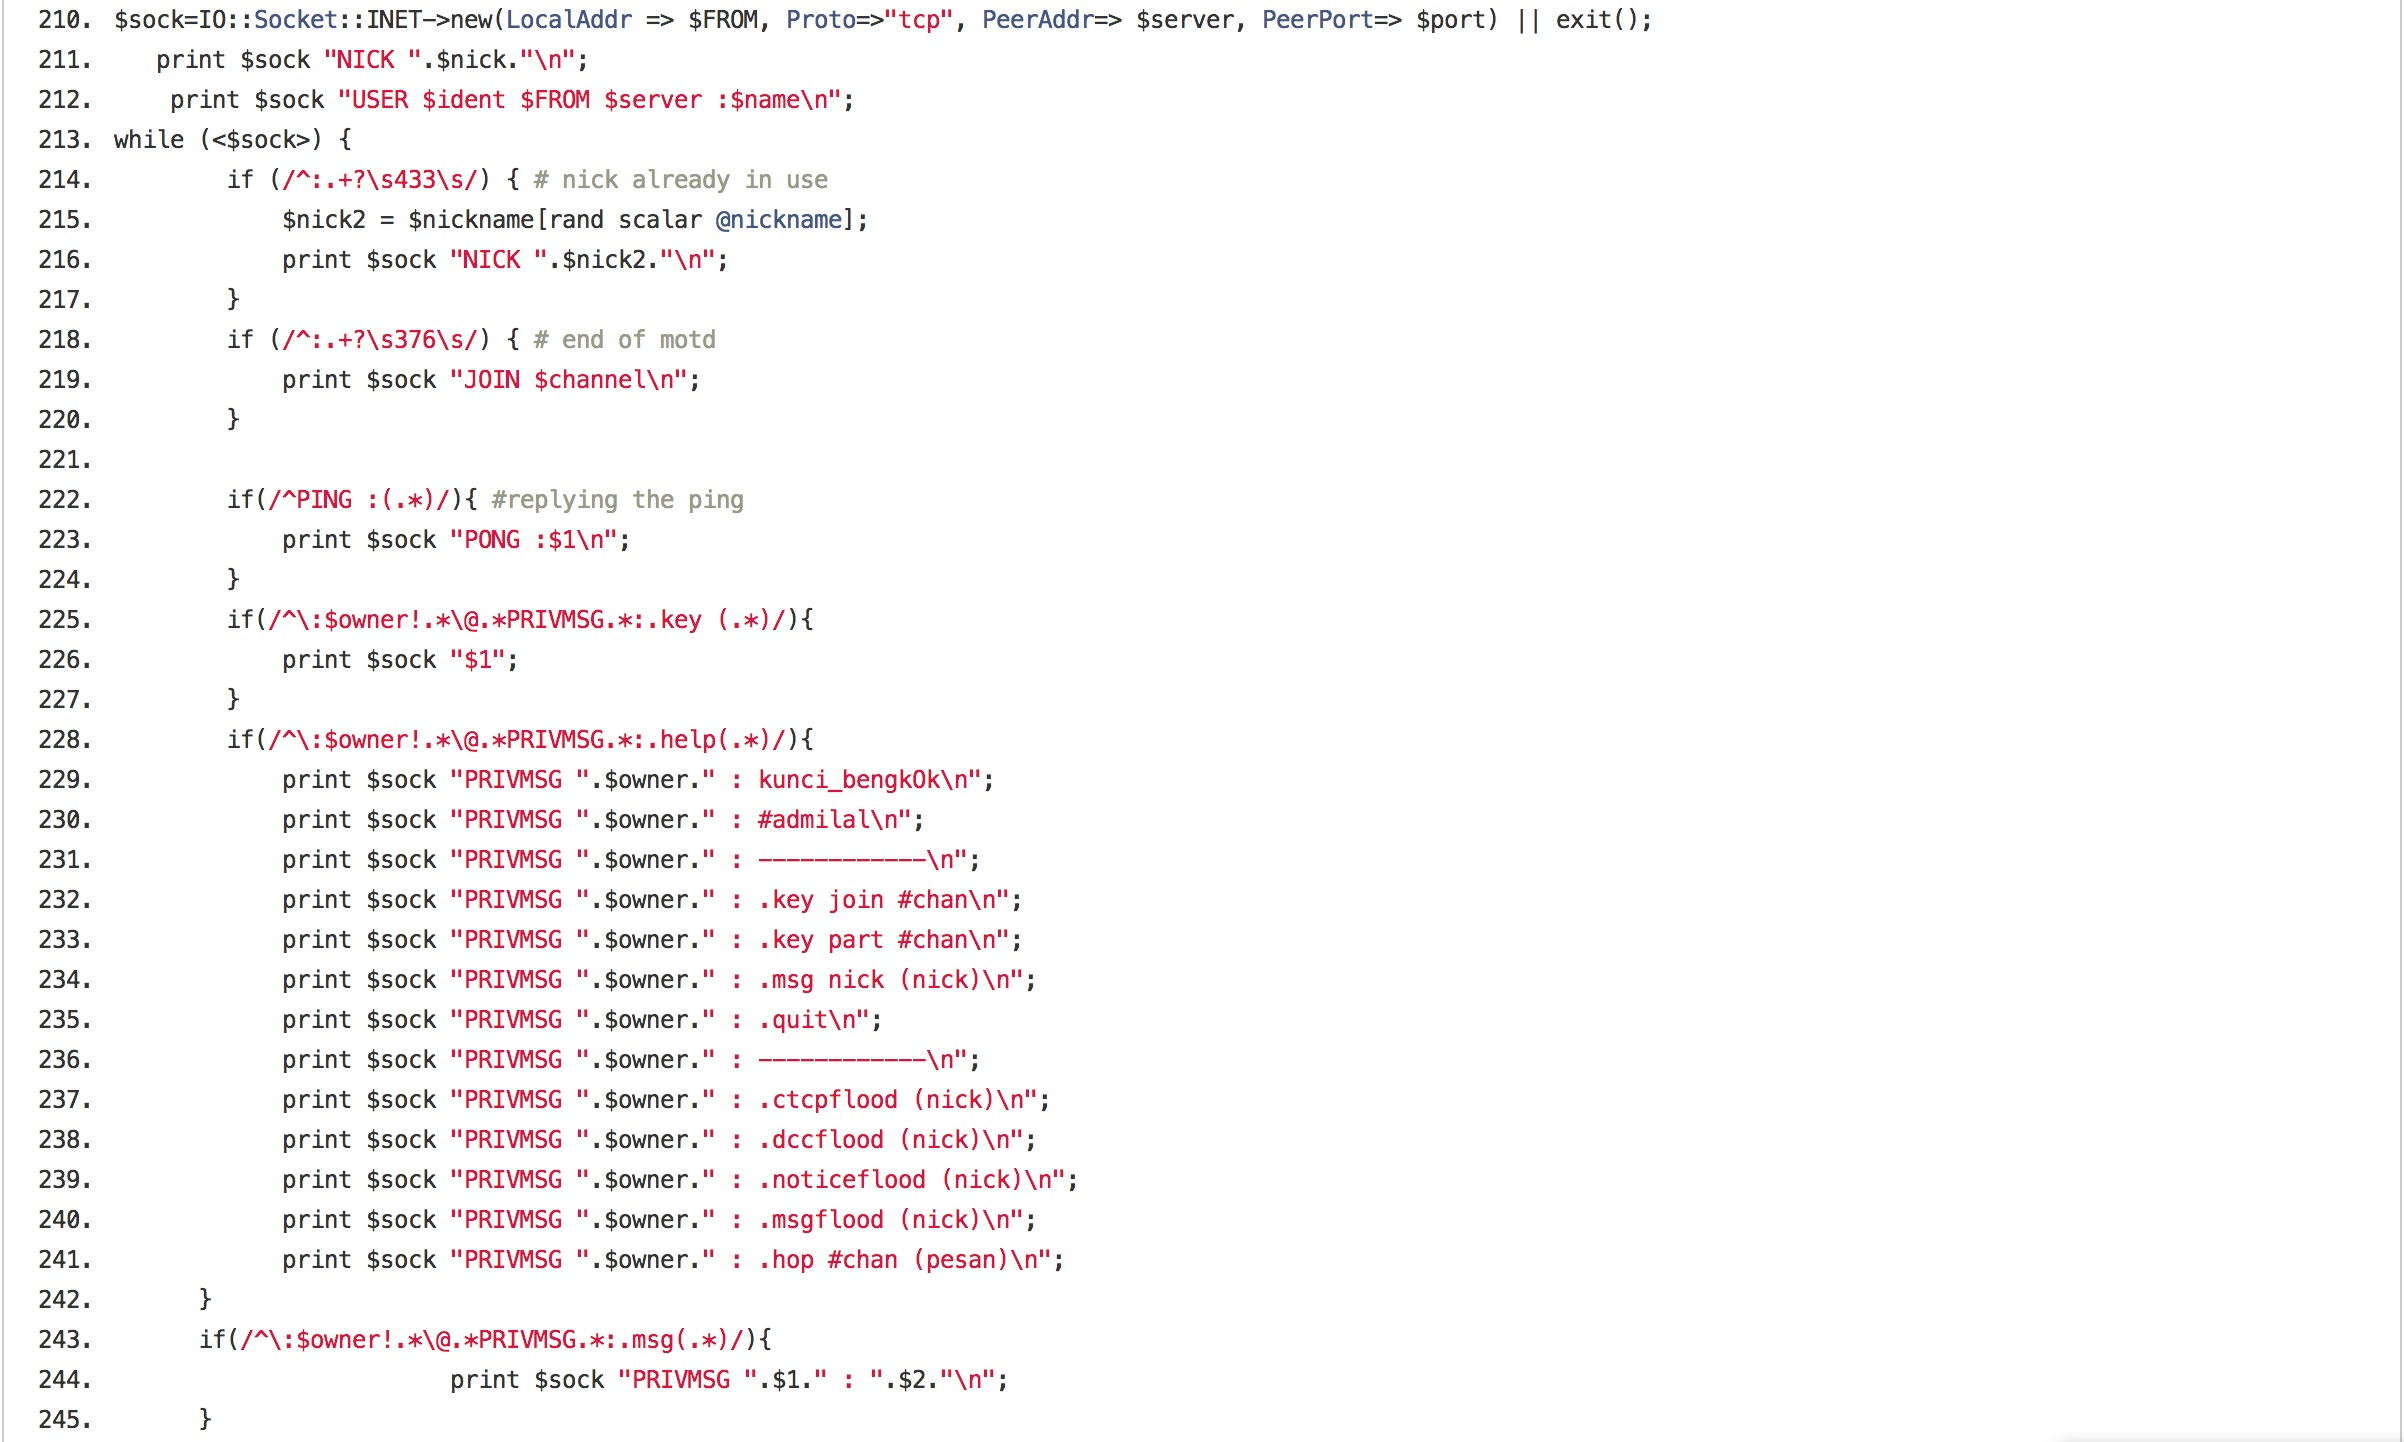
\includegraphics[width=0.8\textwidth]{Images/botnet.jpg}}
\caption{Botnet Initial setup (partial)\label{fig:botnet}}
\end{figure}

\subsection{Phishing Pack}

\begin{quote}
Number of Unique Files: 7445\\
Number of Total Files: 16608\\
Ratio (Unique/Total): 44.8\%
\end{quote}

A phishing pack is a collection of HTML, CSS, javascript files, usually compressed in an archive, aimed to reproduce another website, usually a bank login webpage, in order to trick the victim to insert his credentials inside a webpage. These information are usually logged, while the user is redirected to the right web server (or an error page is displayed). Another script is periodically checking the logs and sending the collected credentials to the criminal.

A victim is usually tricked into accessing the webpage via spamming campaings. During our studies we received several connection attempts with referrer header set to a webmail (like msn, yahoo, aol) or to a forum. While it's impossible for us to understand if the client connecting to the page is a victim or a criminal, and we can't therefore stop the user to insert his credentials, we mitigate the risk by periodically restoring web applications to the original state and by avoiding credentials being transferred from our servers to criminal's ones as we block connections starting from our web servers.

We studied the most common websites reproduced by attackers by means of specific words extraction when analyzing complete phishing packs (that is, packs containing all HTML, javascript and CSS needed for displaying complete pages) and by analyzing URLs requested when analyzing partial packs (packs containing only HTML pages which are requesting CSS and JS scripts from external sources, usually sites they are replicating). Our analysis (ref Figure~\ref{fig:phishGraph}) shows as in more than 50\% of the cases, the replicated website is a bank/money-transfer related login page, like bankofamerica.com or paypal.com, while webmail login pages and e-commerce websites are respectively classified as second and third. Most of the Other section is fulfilled by Social Network login pages, especially Facebook and Twitter websites.

\begin{figure}[H]
\centerline{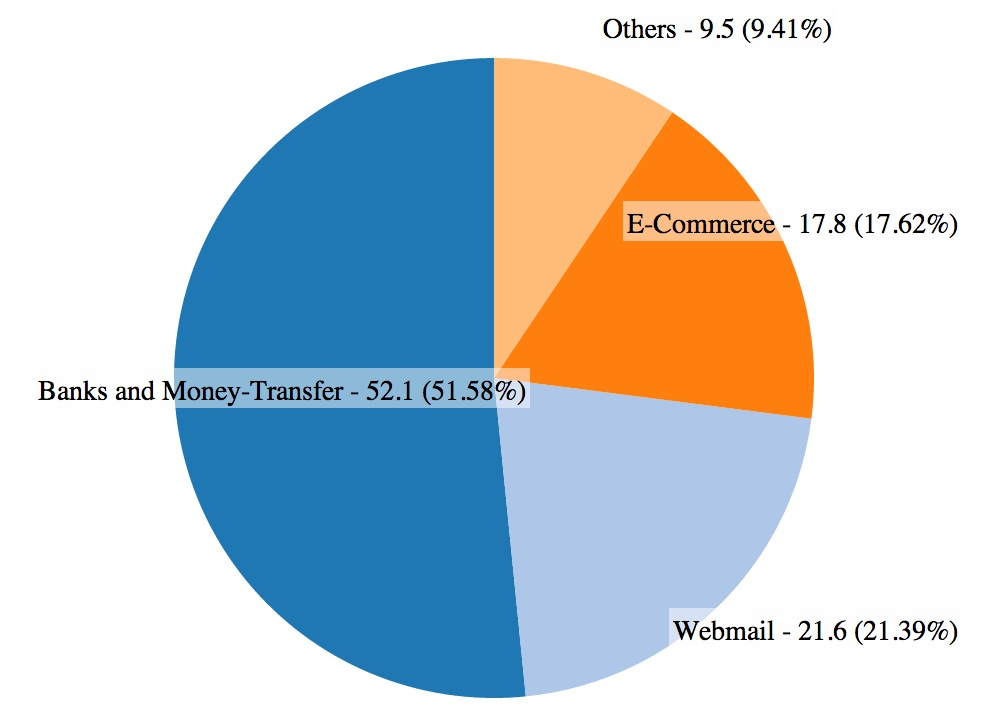
\includegraphics[width=0.8\textwidth]{Images/phishGraph.jpg}}
\caption{Phishing objectives\label{fig:phishGraph}}
\end{figure}

\subsection{Mailer}

\begin{quote}
Number of Unique Files: 11012\\
Number of Total Files: 16324\\
Ratio (Unique/Total): 67.4\%
\end{quote}

A mailer is a category strictly related to a phishing pack: the purpose of such a script, in fact, is to send the same e-mail to a high number of mailboxes. The e-mail is usually a spam message. We can classify spam messages in two categories, according to their purposes: Phishing-inducing messages, where attackers try to impersonate an organization in order to induce the client to click on a link redirecting to a phishing pack and stealing his credentials for that website, and Exploit-campaign messages, where the victim is tricked into clicking on a link redirecting to a malicious website which is performing an exploit toward the client browser (usually activating a Drive-By Download).

Inside this category, we received several examples of files, from very simple scripts which read a list of e-mails and send the same message to all of them, up to something more professional, where the message is slightly changed for every e-mail address (probably for avoiding spam detection filters) and with the possibility to connect to a remote SMTP server, which will deliver outgoing messages on behalf of the script.

In the example in Figure~\ref{fig:mailer} we show a classical example of mailer. The script receives a mail message from the attacker and a list of e-mail addresses, and sends the same e-mail to all of them, using the built-in \emph{sendmail} function from PHP. It's interesting to notice how this script has the possibility to set a FWD header in the e-mail, inducing the client to believe that the e-mail was coming from a real person.

\begin{figure}[H]
\centerline{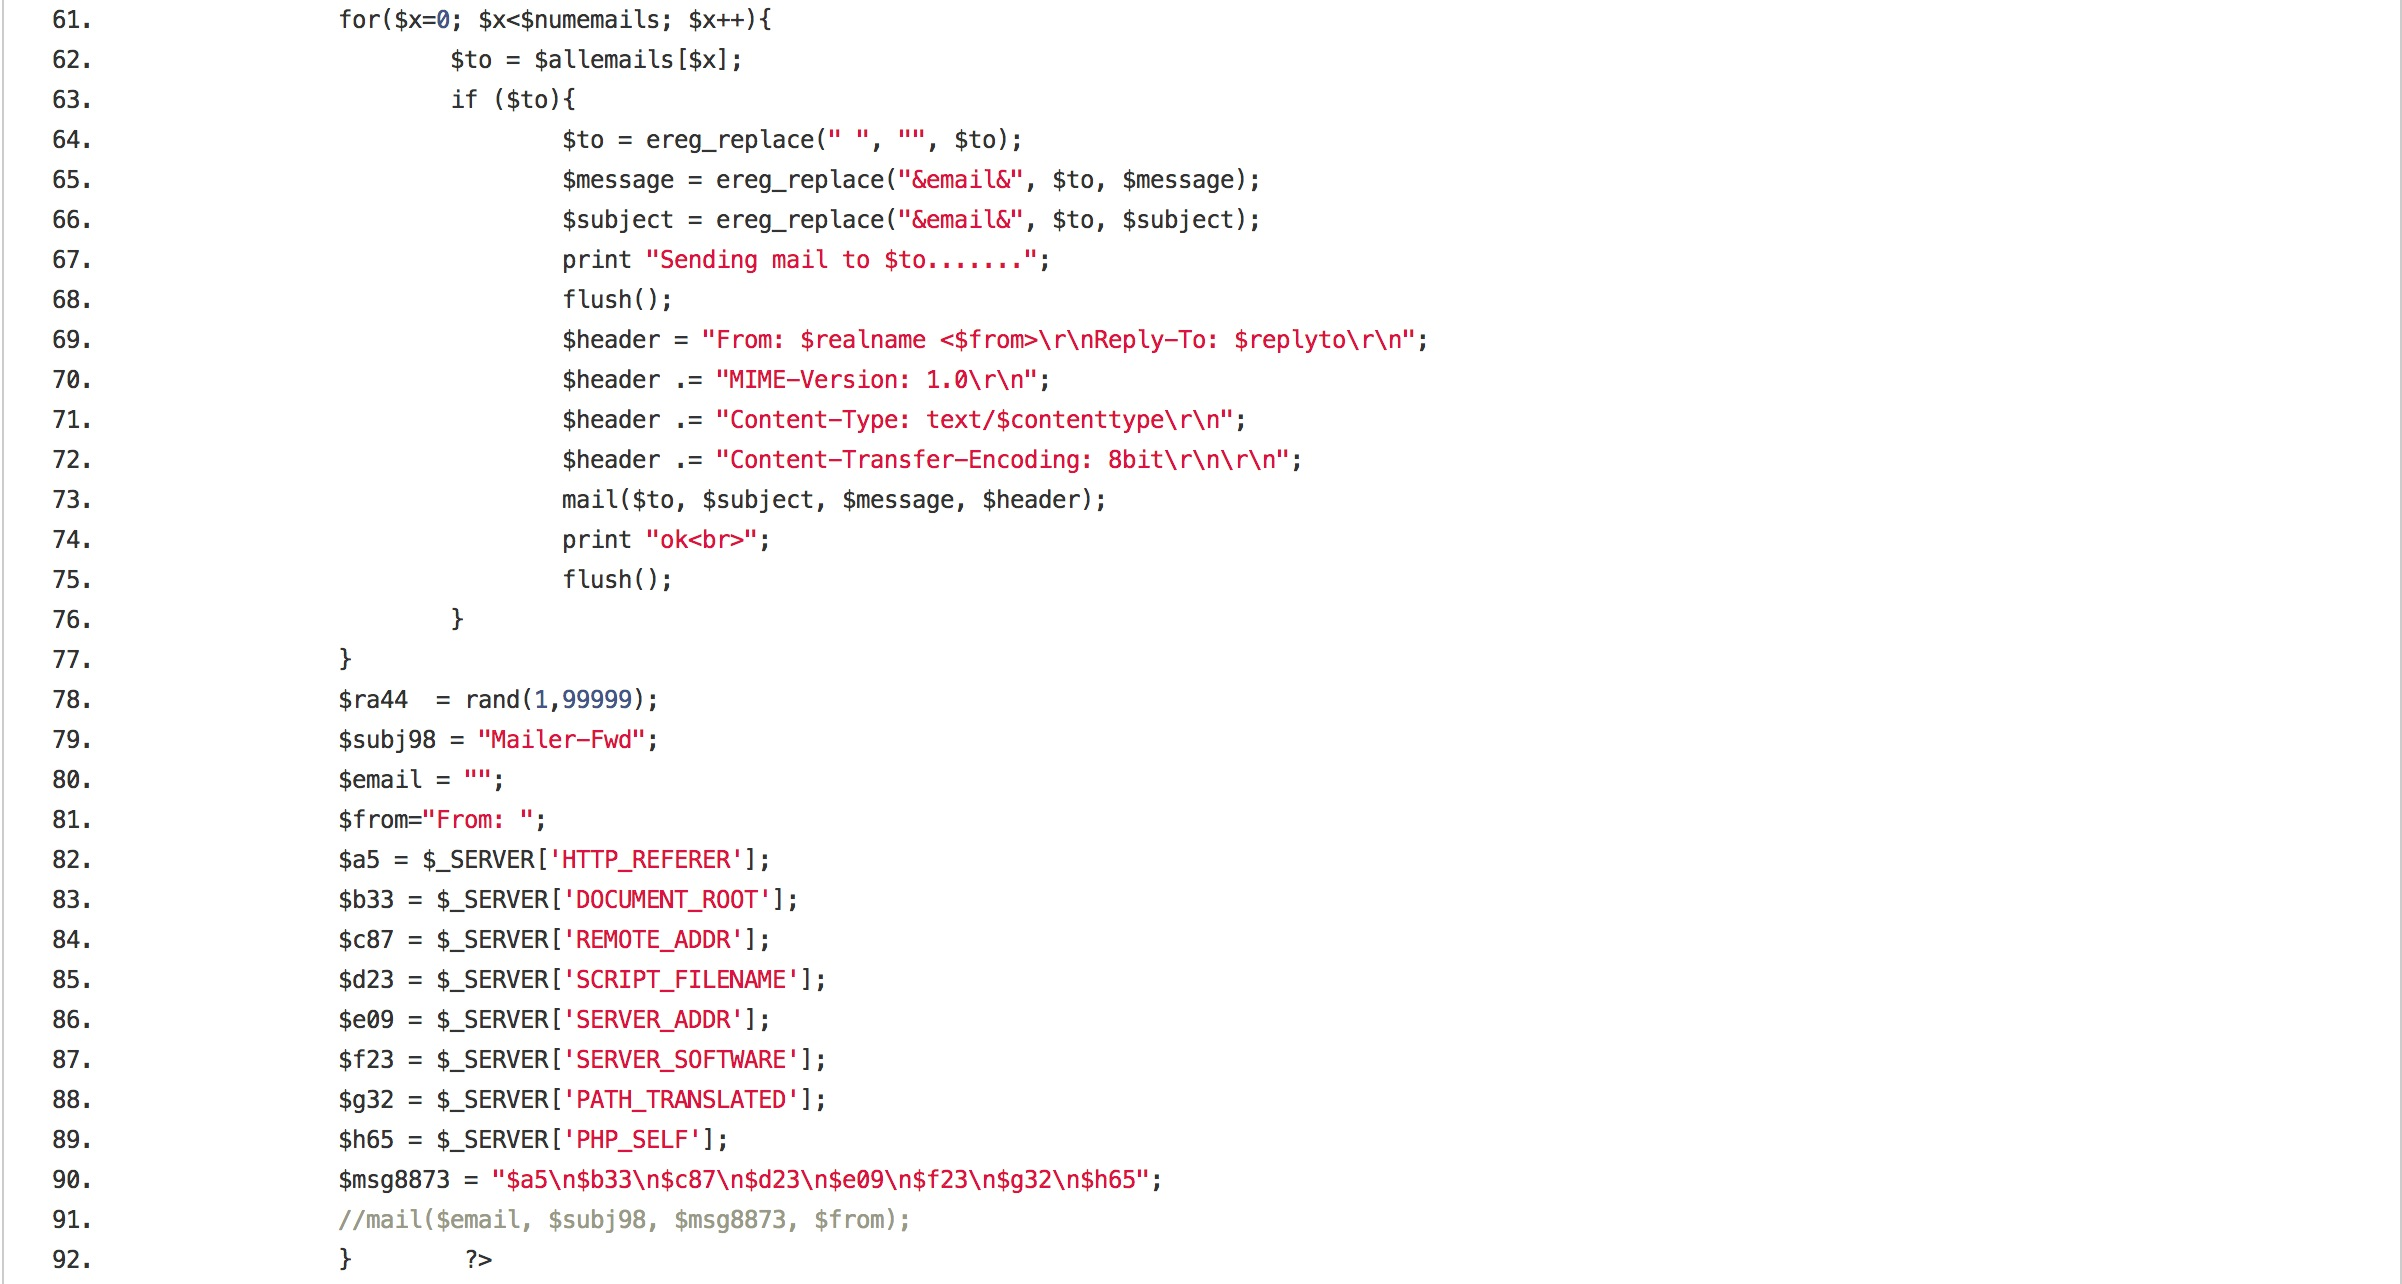
\includegraphics[width=0.8\textwidth]{Images/mailer.jpg}}
\caption{Example of a Mailer sending function\label{fig:mailer}}
\end{figure}

\subsection{Defacement}

\begin{quote}
Number of Unique Files: 12698\\
Number of Total Files: 13023\\
Ratio (Unique/Total): 97.5\%
\end{quote}

Defacement is one the most common purposes attackers have while exploiting a web server. We define defacement as an attack on a website aimed to change the visual appearance of the site. This kind of attack is usually performed on the index.html/index.php webpage, in order to replace the homepage of the website, but because our pages can't be modified, attackers tried to perform defacements using every possible solution to this problem (change of the directoryIndex configuration entry in the php.ini file, symbolic links of webpages etc.).

On a defacement page we can usually find the name of the attacker (often both nickname and actual name), his team (if any), an image/video and a message, which can be goliardic (``your security is low''), insulting or supporting a political/religious cause (Palestinian cause, Kashmir instability etc.). Furthermore, we found in several pages an e-mail address, twitter username, the URL of a blog belonging to the attacker and even a phone number. Attackers seem not to fear any possible legal consequences from their actions, as their country (usually a third world country) have no legislative corpus regarding virtual attacks. Finally, a good number of examples we collected has links to Google Analytics and to Zone-h website \cite{zoneh}. The latter one is a web application tracking defacements happening all over the world and drawing up a ranking of the most active ``defacers'' in the world.

A good example of Defacement can be seen in Figure~\ref{fig:defacement}, performed by a Brazilian Hacking Team from a German IP address.

\begin{figure}[H]
\centerline{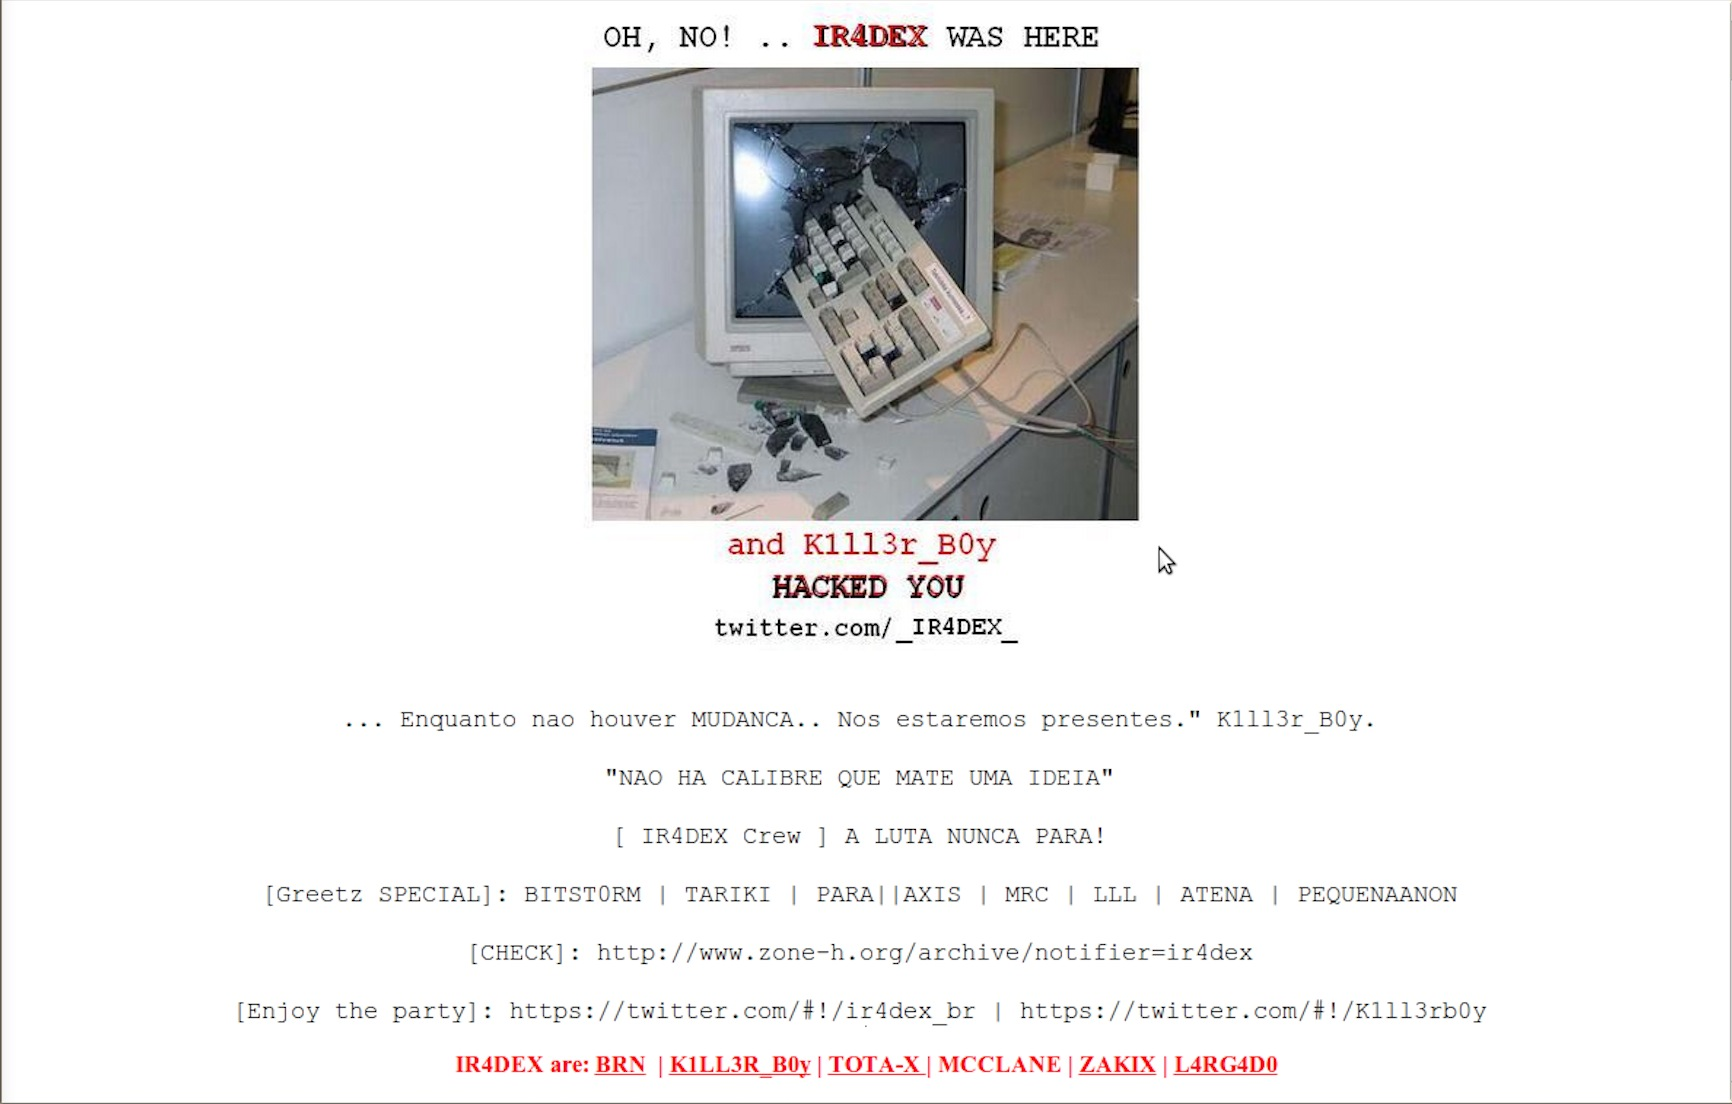
\includegraphics[width=0.8\textwidth]{Images/defacement.jpg}}
\caption{Defacement Page\label{fig:defacement}}
\end{figure}

\subsection{Web Shell}

\begin{quote}
Number of Unique Files: 30522\\
Number of Total Files: 38751\\
Ratio (Unique/Total): 78.8\%
\end{quote}

Uploading a web shell is the most common action attackers performed on our servers during our experiments. A web shell, in fact, is a script (usually written in PHP) able to accept commands and to execute several action on the web server where it is installed. Among these actions, we can usually find remote PHP code execution, remote Shell code execution, information leaking and file upload. Several web shells allow the attacker to send e-mails, performing bruteforce attacks or local exploits. An interesting capability we found in several web shells is the capability of sending an e-mail to the creator of the web shell, notifying of the successful upload. This section of the script is usually obfuscated with respect to the rest of the file, as the creator is generally a different person with respect to the user of the web shell. Furthermore, most of the web shells require some sort of knowledge of the existence of the script before using it, like a password or a specific set of parameters that should be included in the HTTP request.

We analysed web shells we received by comparing them to our set of 17 pre-installed web shells that were installed on one of our web applications. Our web shells can be commonly found in the wild and have been purged from every unwanted parameter, like hidden mail-sending functions, creator names etc. The results of our analysis is shown in Figure~\ref{fig:shellsClusters}. We can see how we managed to identify a good number of clusters, the biggest ones being the cluster of web shells similar to c100 and uploadshell, while other web shells are rarely used during nowadays attacks.
Furthermore, we can see how there are some examples of web shells connected to more than one cluster and which are equidistant from all of them: this kind of shells are actually the result of merging more than one original web shell in order to include functionalities from both of them.


\begin{figure}[H]
\centerline{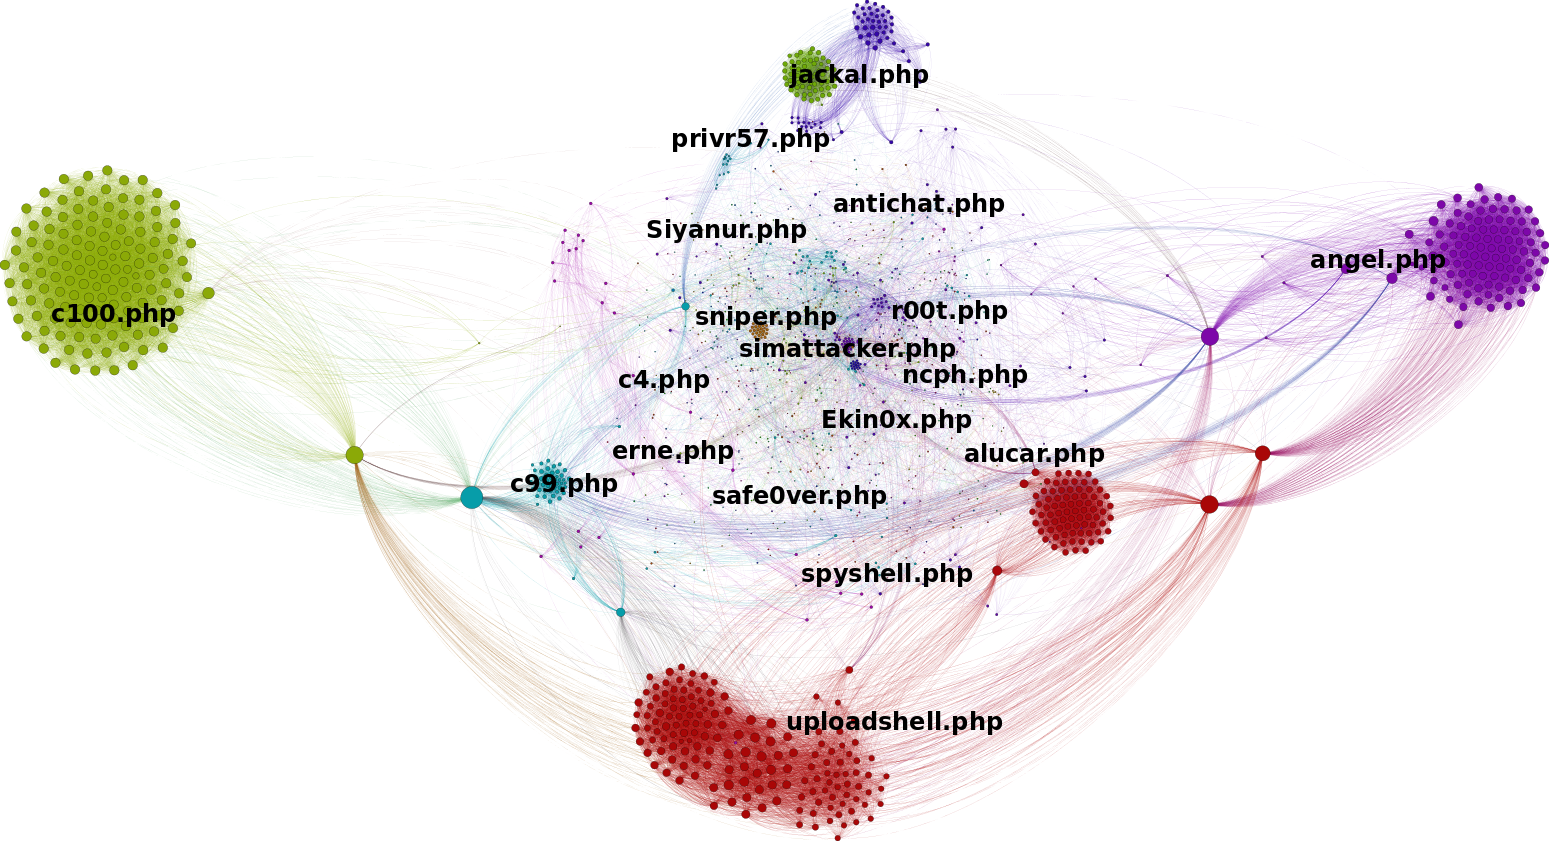
\includegraphics[width=0.8\textwidth]{Images/shellsClusters.png}}
\caption{Web shell clustering (our shells are labeled)\label{fig:shellsClusters}}
\end{figure}
